\documentclass[a4paper]{article}

\def\npart {III}
\def\nterm {Michaelmas}
\def\nyear {2017}
\def\nlecturer {C.\ P.\ Caulfield}
\def\ncourse {Hydrodynamic Stability}

% Imports
\ifx \nextra \undefined
  \usepackage[pdftex,
    hidelinks,
    pdfauthor={Dexter Chua},
    pdfsubject={Cambridge Maths Notes: Part \npart\ - \ncourse},
    pdftitle={Part \npart\ - \ncourse},
  pdfkeywords={Cambridge Mathematics Maths Math \npart\ \nterm\ \nyear\ \ncourse}]{hyperref}
  \title{Part \npart\ - \ncourse}
\else
  \usepackage[pdftex,
    hidelinks,
    pdfauthor={Dexter Chua},
    pdfsubject={Cambridge Maths Notes: Part \npart\ - \ncourse\ (\nextra)},
    pdftitle={Part \npart\ - \ncourse\ (\nextra)},
  pdfkeywords={Cambridge Mathematics Maths Math \npart\ \nterm\ \nyear\ \ncourse\ \nextra}]{hyperref}

  \title{Part \npart\ - \ncourse \\ {\Large \nextra}}
\fi

\author{Lectured by \nlecturer \\\small Notes taken by Dexter Chua}
\date{\nterm\ \nyear}

\usepackage{alltt}
\usepackage{amsfonts}
\usepackage{amsmath}
\usepackage{amssymb}
\usepackage{amsthm}
\usepackage{booktabs}
\usepackage{caption}
\usepackage{enumitem}
\usepackage{fancyhdr}
\usepackage{graphicx}
\usepackage{mathtools}
\usepackage{microtype}
\usepackage{multirow}
\usepackage{pdflscape}
\usepackage{pgfplots}
\usepackage{siunitx}
\usepackage{tabularx}
\usepackage{tikz}
\usepackage{tkz-euclide}
\usepackage[normalem]{ulem}
\usepackage[all]{xy}

\pgfplotsset{compat=1.12}

\pagestyle{fancyplain}
\lhead{\emph{\nouppercase{\leftmark}}}
\ifx \nextra \undefined
  \rhead{
    \ifnum\thepage=1
    \else
      \npart\ \ncourse
    \fi}
\else
  \rhead{
    \ifnum\thepage=1
    \else
      \npart\ \ncourse\ (\nextra)
    \fi}
\fi
\usetikzlibrary{arrows}
\usetikzlibrary{decorations.markings}
\usetikzlibrary{decorations.pathmorphing}
\usetikzlibrary{positioning}
\usetikzlibrary{fadings}
\usetikzlibrary{intersections}
\usetikzlibrary{cd}

\newcommand*{\Cdot}{\raisebox{-0.25ex}{\scalebox{1.5}{$\cdot$}}}
\newcommand {\pd}[2][ ]{
  \ifx #1 { }
    \frac{\partial}{\partial #2}
  \else
    \frac{\partial^{#1}}{\partial #2^{#1}}
  \fi
}

% Theorems
\theoremstyle{definition}
\newtheorem*{aim}{Aim}
\newtheorem*{axiom}{Axiom}
\newtheorem*{claim}{Claim}
\newtheorem*{cor}{Corollary}
\newtheorem*{defi}{Definition}
\newtheorem*{eg}{Example}
\newtheorem*{fact}{Fact}
\newtheorem*{law}{Law}
\newtheorem*{lemma}{Lemma}
\newtheorem*{notation}{Notation}
\newtheorem*{prop}{Proposition}
\newtheorem*{thm}{Theorem}

\renewcommand{\labelitemi}{--}
\renewcommand{\labelitemii}{$\circ$}
\renewcommand{\labelenumi}{(\roman{*})}

\let\stdsection\section
\renewcommand\section{\newpage\stdsection}

% Strike through
\def\st{\bgroup \ULdepth=-.55ex \ULset}

% Maths symbols
\newcommand{\bra}{\langle}
\newcommand{\ket}{\rangle}

\newcommand{\N}{\mathbb{N}}
\newcommand{\Z}{\mathbb{Z}}
\newcommand{\Q}{\mathbb{Q}}
\renewcommand{\H}{\mathbb{H}}
\newcommand{\R}{\mathbb{R}}
\newcommand{\C}{\mathbb{C}}
\newcommand{\Prob}{\mathbb{P}}
\renewcommand{\P}{\mathbb{P}}
\newcommand{\E}{\mathbb{E}}
\newcommand{\F}{\mathbb{F}}
\newcommand{\cU}{\mathcal{U}}
\newcommand{\RP}{\mathbb{RP}}
\newcommand{\CP}{\mathbb{CP}}

\newcommand{\ph}{\,\cdot\,}

\DeclareMathOperator{\sech}{sech}
\DeclareMathOperator{\cosech}{cosech}
\DeclareMathOperator{\cosec}{cosec}

\DeclareMathOperator{\covol}{covol}
\DeclareMathOperator{\vol}{vol}

\let\Im\relax
\let\Re\relax
\DeclareMathOperator{\Im}{Im}
\DeclareMathOperator{\Re}{Re}
\DeclareMathOperator{\im}{im}
\DeclareMathOperator{\image}{image}
\DeclareMathOperator{\Ann}{Ann}

\DeclareMathOperator*{\res}{res}
\DeclareMathOperator{\Res}{Res}
\DeclareMathOperator{\Ind}{Ind}

\DeclareMathOperator{\tr}{tr}
\DeclareMathOperator{\diag}{diag}
\DeclareMathOperator{\rank}{rank}
\DeclareMathOperator{\card}{card}
\DeclareMathOperator{\spn}{span}
\DeclareMathOperator{\adj}{adj}

\DeclareMathOperator{\erf}{erf}
\DeclareMathOperator{\erfc}{erfc}

\DeclareMathOperator{\ord}{ord}
\DeclareMathOperator{\Sym}{Sym}

\DeclareMathOperator{\sgn}{sgn}
\DeclareMathOperator{\orb}{orb}
\DeclareMathOperator{\stab}{stab}
\DeclareMathOperator{\ccl}{ccl}

\DeclareMathOperator{\lcm}{lcm}
\DeclareMathOperator{\hcf}{hcf}

\DeclareMathOperator{\Int}{Int}
\DeclareMathOperator{\id}{id}

\DeclareMathOperator{\betaD}{beta}
\DeclareMathOperator{\gammaD}{gamma}
\DeclareMathOperator{\Poisson}{Poisson}
\DeclareMathOperator{\binomial}{binomial}
\DeclareMathOperator{\multinomial}{multinomial}
\DeclareMathOperator{\Bernoulli}{Bernoulli}
\DeclareMathOperator{\like}{like}

\DeclareMathOperator{\var}{var}
\DeclareMathOperator{\cov}{cov}
\DeclareMathOperator{\bias}{bias}
\DeclareMathOperator{\mse}{mse}
\DeclareMathOperator{\corr}{corr}

\DeclareMathOperator{\otp}{otp}
\DeclareMathOperator{\dom}{dom}

\DeclareMathOperator{\Root}{Root}
\DeclareMathOperator{\supp}{supp}
\DeclareMathOperator{\rel}{rel}
\DeclareMathOperator{\Hom}{Hom}
\DeclareMathOperator{\Aut}{Aut}
\DeclareMathOperator{\Gal}{Gal}
\DeclareMathOperator{\Mat}{Mat}
\DeclareMathOperator{\End}{End}
\DeclareMathOperator{\Char}{char}
\DeclareMathOperator{\ev}{ev}
\DeclareMathOperator{\St}{St}
\DeclareMathOperator{\Lk}{Lk}
\DeclareMathOperator{\disc}{disc}
\DeclareMathOperator{\Isom}{Isom}
\DeclareMathOperator{\length}{length}
\DeclareMathOperator{\energy}{energy}
\DeclareMathOperator{\area}{area}
\DeclareMathOperator{\Syl}{Syl}
\DeclareMathOperator{\cl}{cl}
\DeclareMathOperator{\fix}{fix}

\newcommand{\GL}{\mathrm{GL}}
\newcommand{\SL}{\mathrm{SL}}
\newcommand{\PGL}{\mathrm{PGL}}
\newcommand{\PSL}{\mathrm{PSL}}
\newcommand{\PSU}{\mathrm{PSU}}
\newcommand{\Or}{\mathrm{O}}
\newcommand{\SO}{\mathrm{SO}}
\newcommand{\U}{\mathrm{U}}
\newcommand{\SU}{\mathrm{SU}}

\renewcommand{\d}{\mathrm{d}}
\newcommand{\D}{\mathrm{D}}

\tikzset{->/.style = {decoration={markings,
                                  mark=at position 1 with {\arrow[scale=2]{latex'}}},
                      postaction={decorate}}}
\tikzset{<-/.style = {decoration={markings,
                                  mark=at position 0 with {\arrowreversed[scale=2]{latex'}}},
                      postaction={decorate}}}
\tikzset{<->/.style = {decoration={markings,
                                   mark=at position 0 with {\arrowreversed[scale=2]{latex'}},
                                   mark=at position 1 with {\arrow[scale=2]{latex'}}},
                       postaction={decorate}}}
\tikzset{->-/.style = {decoration={markings,
                                   mark=at position #1 with {\arrow[scale=2]{latex'}}},
                       postaction={decorate}}}
\tikzset{-<-/.style = {decoration={markings,
                                   mark=at position #1 with {\arrowreversed[scale=2]{latex'}}},
                       postaction={decorate}}}

\tikzset{circ/.style = {fill, circle, inner sep = 0, minimum size = 3}}
\tikzset{mstate/.style={circle, draw, blue, text=black, minimum width=0.7cm}}

\definecolor{mblue}{rgb}{0.2, 0.3, 0.8}
\definecolor{morange}{rgb}{1, 0.5, 0}
\definecolor{mgreen}{rgb}{0.1, 0.4, 0.2}
\definecolor{mred}{rgb}{0.5, 0, 0}

\def\drawcirculararc(#1,#2)(#3,#4)(#5,#6){%
    \pgfmathsetmacro\cA{(#1*#1+#2*#2-#3*#3-#4*#4)/2}%
    \pgfmathsetmacro\cB{(#1*#1+#2*#2-#5*#5-#6*#6)/2}%
    \pgfmathsetmacro\cy{(\cB*(#1-#3)-\cA*(#1-#5))/%
                        ((#2-#6)*(#1-#3)-(#2-#4)*(#1-#5))}%
    \pgfmathsetmacro\cx{(\cA-\cy*(#2-#4))/(#1-#3)}%
    \pgfmathsetmacro\cr{sqrt((#1-\cx)*(#1-\cx)+(#2-\cy)*(#2-\cy))}%
    \pgfmathsetmacro\cA{atan2(#2-\cy,#1-\cx)}%
    \pgfmathsetmacro\cB{atan2(#6-\cy,#5-\cx)}%
    \pgfmathparse{\cB<\cA}%
    \ifnum\pgfmathresult=1
        \pgfmathsetmacro\cB{\cB+360}%
    \fi
    \draw (#1,#2) arc (\cA:\cB:\cr);%
}
\newcommand\getCoord[3]{\newdimen{#1}\newdimen{#2}\pgfextractx{#1}{\pgfpointanchor{#3}{center}}\pgfextracty{#2}{\pgfpointanchor{#3}{center}}}

\def\Xint#1{\mathchoice
   {\XXint\displaystyle\textstyle{#1}}%
   {\XXint\textstyle\scriptstyle{#1}}%
   {\XXint\scriptstyle\scriptscriptstyle{#1}}%
   {\XXint\scriptscriptstyle\scriptscriptstyle{#1}}%
   \!\int}
\def\XXint#1#2#3{{\setbox0=\hbox{$#1{#2#3}{\int}$}
     \vcenter{\hbox{$#2#3$}}\kern-.5\wd0}}
\def\ddashint{\Xint=}
\def\dashint{\Xint-}


\usepackage{gnuplottex}
\newcommand\Ra{\mathrm{Ra}}
\renewcommand\Pr{\mathrm{Pr}}
\begin{document}
\maketitle
{\small
\setlength{\parindent}{0em}
\setlength{\parskip}{1em}
Developing an understanding by which ``small'' perturbations grow, saturate and modify fluid flows is central to addressing many challenges of interest in fluid mechanics. Furthermore, many applied mathematical tools of much broader relevance have been developed to solve hydrodynamic stability problems, and hydrodynamic stability theory remains an exceptionally active area of research, with several exciting new developments being reported over the last few years.

In this course, an overview of some of these recent developments will be presented. After an introduction to the general concepts of flow instability, presenting a range of examples, the major content of this course will be focussed on the broad class of flow instabilities where velocity ``shear'' and fluid inertia play key dynamical roles. Such flows, typically characterised by sufficiently“high” Reynolds number $Ud/\nu$, where $U$ and $d$ are characteristic velocity and length scales of the flow, and $\nu$ is the kinematic viscosity of the fluid, are central to modelling flows in the environment and industry. They typically demonstrate the key role played by the redistribution of vorticity within the flow, and such vortical flow instabilities often trigger the complex, yet hugely important process of ``transition to turbulence''.

A hierarchy of mathematical approaches will be discussed to address a range of ``stability'' problems, from more traditional concepts of ``linear'' infinitesimal normal mode perturbation energy growth on laminar parallel shear flows to transient, inherently nonlinear perturbation growth of general measures of perturbation magnitude over finite time horizons where flow geometry and/or fluid properties play a dominant role. The course will also discuss in detail physical interpretations of the various flow instabilities considered, as well as the industrial and environmental application of the results of the presented mathematical analyses

\subsubsection*{Pre-requisites}
Elementary concepts from undergraduate real analysis. Some knowledge of complex analysis would be advantageous (e.g.\ the level of IB Complex Analysis/Methods). No knowledge of functional analysis is assumed.
}
\tableofcontents

\section{Linear stability analysis}
\subsection{Rayleigh--Taylor instability}
In this section, we would like to investigate the stability of a surface between two fluids:
\begin{center}
  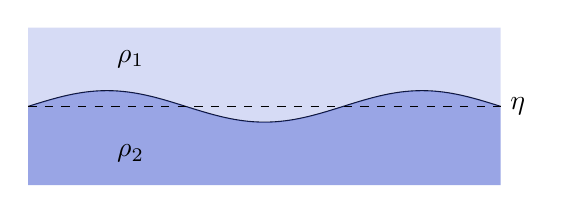
\begin{tikzpicture}
    \draw (-3, 0) sin (-2, 0.2) cos (-1, 0) sin (0, -0.2) cos (1, 0) sin (2, 0.2) cos (3, 0) node [right] {$\eta$};
    \fill [mblue, opacity=0.5] (-3, -1) -- (-3, 0) sin (-2, 0.2) cos (-1, 0) sin (0, -0.2) cos (1, 0) sin (2, 0.2) cos (3, 0) -- (3, -1);
    \fill [mblue, opacity=0.2] (-3, 1) -- (-3, 0) sin (-2, 0.2) cos (-1, 0) sin (0, -0.2) cos (1, 0) sin (2, 0.2) cos (3, 0) -- (3, 1);

    \draw [dashed] (-3, 0) -- (3, 0);
    \node at (-1.7, -0.6) {$\rho_2$};
    \node at (-1.7, 0.6) {$\rho_1$};
  \end{tikzpicture}
\end{center}
We assume the two fluids have densities $\rho_1$ and $\rho_2$, and are separated by a smooth interface parametrized by the deviation $\eta$.

Recall that the Navier--Stokes equations for an incompressible fluid are
\[
  \rho\left(\frac{\partial \mathbf{u}}{\partial t} + \mathbf{u} \cdot \nabla \mathbf{u}\right) = - \nabla P- g \rho \hat{\mathbf{z}} + \mu \nabla^2 \mathbf{u},\quad \nabla \cdot \mathbf{u} = 0.
\]
Usually, when doing fluid mechanics, we assume density is constant, and divide the whole equation across by $\rho$. We can then forget the existence of $\rho$ and carry on. We can also get rid of the gravity term. We know that the force of gravity is balanced out by a hydrostatic pressure gradient. More precisely, we can write
\[
  P = P_h(z) + p (x, t),
\]
where $P_h$ satisfies
\[
  \frac{\partial P_h}{\partial z} = -g\rho.
\]
We can then write our equation as
\[
  \frac{\partial \mathbf{u}}{\partial t} + \mathbf{u}\cdot \nabla \mathbf{u} = - \nabla \left(\frac{p}{\rho}\right) + \nu \nabla^2 \mathbf{u}.
\]
To do all of these, we must assume that the density $\rho$ is constant, but this is clearly not the case when we have tow distinct fluids.

Since it is rather difficult to move forward without making \emph{any} simplifying assumptions, we shall focus on the case of inviscid fluids, so that we take $\nu = 0$. We will also assume that the fluid is irrotational. In this case, it is convenient to use the vector calculus identity
\[
  \mathbf{u} \cdot \nabla \mathbf{u} = \nabla \left(\frac{1}{2}|\mathbf{u}|^2\right) - \mathbf{u} \times (\nabla \times \mathbf{u}),
\]
where we can now drop the second term. Moreover, since $\nabla \times \mathbf{u} = 0$, Stokes' theorem allows us to write $\mathbf{u} = \nabla \phi$ for some \term{velocity potential} $\phi$. Finally, in each separate region, the density $\rho$ is constant. So we can now write
\[
  \nabla \left(\rho \frac{\partial \phi}{\partial t} + \frac{1}{2} \rho |\nabla \phi|^2 + P + g \rho z\right) = 0.
\]
This is \term{Bernoulli's theorem}.

Applying these to our scenario, since we have two fluids, we have two separate velocity potentials $\phi_1, \phi_2$ for the two two regions. Both of these independently satisfy the incompressibility hypothesis
\[
  \nabla^2\phi_{1, 2} = 0.
\]
Bernoulli's theorem tells us the quantity
\[
  \rho \frac{\partial \phi}{\partial t} + \frac{1}{2} \rho |\nabla \phi|^2 + P + g \rho z
\]
should be constant across the fluid. Our investigation will not use the full equation. All we will need is that this quantity matches at the interface, so that we have
\[
  \left.\rho_1 \frac{\partial \phi_1}{\partial t} + \frac{1}{2} \rho_1 |\nabla \phi_1|^2 + P_1 + g \rho_1 \eta\right|_{z = \eta} = \left.\rho_2 \frac{\partial \phi_2}{\partial t} + \frac{2}{2} \rho_2 |\nabla \phi_2|^2 + P_2 + g \rho_2 \eta\right|_{z = \eta}.
\]
To understand the interface, we must impose boundary conditions. First of all the vertical velocities of the fluids must match with the interface, so we impose the \term{kinematic boundary condition}
\[
  \left.\frac{\partial \phi_1}{\partial z} \right|_{z = \eta} = \left.\frac{\partial \phi_2}{\partial z} \right|_{z = \eta} = \frac{\D \eta}{\D t},
\]
where
\[
  \D = \frac{\partial}{\partial t} + \mathbf{u} \cdot \nabla
\]
We also make another, perhaps dubious boundary condition, namely that the pressure is continuous along the interface. This does not hold at all interfaces. For example, if we have a balloon, then the pressure inside is greater than the pressure outside, since that is what holds the balloon up. In this case, it is the rubber that is exerting a force to maintain the pressure difference. In our case, we only have two fluids meeting, and there is no reason to assume a discontinuity in pressure, and thus we shall assume it is continuous. If you are not convinced, this is good, and we shall later see this is indeed a dubious assumption.

But assuming it for the moment, this allows us to simplify our Bernoulli's theorem to give
\[
  \rho_1 \frac{\partial \phi_1}{\partial t} + \frac{1}{2} \rho_1 |\nabla \phi_1|^2 + g \rho_1 \eta = \rho_2 \frac{\partial \phi_2}{\partial t} + \frac{2}{2} \rho_2 |\nabla \phi_2|^2 + g \rho_2 \eta.
\]
There is a final boundary condition that is specific to our model. What we are going to do is that we will start with a flat, static solution with $\mathbf{u} = 0$ and $\eta = 0$. We then perturb $\eta$ a bit, and see what happens to our fluid. In particular, we want to see if the perturbation is stable.

Since we expect the interesting behaviour to occur only near the interface, we make the assumption that there is no velocity in the far field, i.e.\ $\phi_1 \to 0$ as $z \to \infty$ and $\phi_2 \to 0$ as $z \to-\infty$ (and similarly for the derivatives). For simplicity, we also assume there is no $y$ dependence.

We now have equations and boundary conditions, so we can solve them. But these equations are pretty nasty and non-linear. At this point, one sensible approach is to linearize the equations by assuming everything is small. In addition to assuming that $\eta$ is small, we also need to assume that various derivatives such as $\nabla \phi$ are small, so that we can drop all second-order terms. Since $\eta$ is small, the value of, say, $\frac{\partial \phi_1}{\partial z}$ at $\eta$ should be similar to that at $\eta = 0$. Since $\frac{\partial \phi_1}{\partial z}$ itself is already assumed to be small, the difference would be second order in smallness.

So we replace all evaluations at $\eta$ with evaluations at $z = 0$. We are then left with the collection of $3$ equations
\begin{align*}
  \nabla^2 \phi_{1, 2} &= 0\\
  \left.\frac{\partial \phi_{1, 2}}{\partial z}\right|_{z = 0} &= \eta_t\\
  \left.\rho_1 \frac{\partial \phi_1}{\partial t} + g \rho_1 \eta \right|_{z = 0} &= \left.\rho_2 \frac{\partial \phi_2}{\partial t} + g \rho_2 \eta \right|_{z = 0}.
\end{align*}

This is a nice linear problem, and we can analyze the Fourier modes of the solutions. We plug in an ansatz
\begin{align*}
  \phi_{1, 2}(x, z, t) &= \hat{\phi}_{1, 2}(z) e^{i(kx - \omega t)}\\
  \eta(x, t) &= B e^{i(kx - \omega t)}.
\end{align*}
Substituting into Laplace's equation gives
\[
  \hat{\phi}_{1, 2} - k^2 \hat{\phi}_{1, 2} = 0.
\]
Using the far field boundary conditions, we see that we have a family of solutions
\[
  \hat{\phi}_1 = A_1 e^{-kz},\quad \hat{\phi}_2 = A_2 e^{kz}.
\]
The kinematic boundary condition tells us we must have
\[
  \hat{\phi}_{1, 2}'(0) = -i\omega B.
\]
We can solve this to get
\[
  B = \frac{k A_1}{i \omega} = - \frac{kA_2}{ i \omega}.
\]
In particular, we must have $A \equiv A_1 = - A_2$. We can then write
\[
  \eta = \frac{kA}{i\omega} e^{ik(kx - \omega t)}.
\]
Plugging these into the final equation gives us
\[
  \rho_1 (-i\omega A) + g \rho_1 \frac{k A}{i \omega} = \rho_2 i \omega A + g \rho_2 \frac{kA}{i \omega}.
\]
Crucially, we can cancel the $A$ throughout the equation, and gives us a result independent of $A$. This is, after all, the point of linearization. Solving this gives us a \term{dispersion relation} relating the frequency (or phase speed $c_p = \omega/k$) to the wavenumber:
\[
  \omega^2 = \frac{g(\rho_2 - \rho_1)k}{\rho_1 + \rho_2}.
\]
If $\rho_2 \gg \rho_1$, then this reduces to $\omega^2 \approx gk$, and this is the usual dispersion relation for deep water waves. On the other hand, if $\rho_2 - \rho_1 > 0$ is small, this can lead to waves of rather low frequency, which is something we can observe in cocktails, apparently.

But nothing in our analysis actually required $\rho_2 > \rho_1$. Suppose we had $\rho_1 > \rho_2$. This amounts to putting the heavier fluid on top of the lighter one. Anyone who has tried to turn a cup of water upside down will know this is highly unstable. Can we see this from our analysis?

If $\rho_1 < \rho_2$, then $\omega$ has to be imaginary. We shall write it as $\omega = \pm i \sigma$, where $\sigma > 0$. We can then compute
\[
  \sigma = \sqrt{\frac{g(\rho_1 - \rho_2)k}{\rho_1 + \rho_2}}.
\]
Writing out our expression for $\phi_{1, 2}$, we see that there are $e^{\pm \sigma t}$ terms, and the $e^{\sigma t}$ term dominates in the long run, causing $\phi_{1, 2}$ to grow exponentially. This is the \emph{Rayleigh--Taylor instability}.

There is more to say about the instability. As the wavelength decreases, $k$ increases, and we see that $\sigma$ increases as well. Thus, we see that short-scale perturbations blow up exponentially much more quickly, which means the system is not very well-posed. This is the \term{ultra-violet catastrophe}. Of course, we should not trust our model here. Recall that in our simplifying assumptions, we not only assumed that the amplitudes of our $\phi$ and $\eta$ were small, but also that their derivatives were small. The large $k$ behaviour gives us large $x$ derivatives, and so we have to take into account the higher order terms as well.

But we can also provide physical reasons for why small scales perturbations should be suppressed by such a system. In our model, we assumed there is no surface tension. Surface tension quantifies the tendency of interfaces between fluids to minimize surface area. We know that small-scale variations will cause a large surface area, and so the surface tension will suppress these variations. Mathematically, what the surface allows for is a pressure jump across the interface.

Surface tension is quantified by $\gamma$, the force per unit length. This has dimensions $[\gamma] = MT^{-1}$. Empirically, we observe that the pressure difference across the interface is
\[
  \Delta p = - \gamma \nabla \cdot \hat{\mathbf{n}} = 2 \gamma H = \gamma \left(\frac{1}{R_x} + \frac{1}{R_y}\right),
\]
where $\hat{\mathbf{n}}$ is the unit normal and $H$ is the \term{mean curvature}. This is an empirical result.

Again, we assume no dependence in the $y$ direction, so we have a cylindrical interface with a single radius of curvature. Linearizing, we have a pressure difference of
\[
  (P_2 - P_1) |_{z = \eta} = \frac{\gamma}{R_x} = - \gamma \frac{\frac{\partial^2 \eta}{\partial x^2}}{\left(1 + \left(\frac{\partial \eta}{\partial x}\right)^2\right)^{3/2}} \approx -\gamma \frac{\partial^2 \eta}{\partial x^2}.
\]
Therefore the (linearized) dynamic boundary condition becomes
\[
  \left.\rho_1 \frac{\partial \phi_1}{\partial t} + g \rho_1 \eta\right|_{z =0 } + \gamma \frac{\partial^2 \eta}{\partial x^2} = \left. \rho_2 \frac{\partial \phi_2}{\partial t} + g \rho_2 \eta\right|_{z = 0}.
\]
If we run the previous analysis again, we find a dispersion relation of
\[
  \omega^2 = \frac{g(\rho_2 - \rho_1)k + \gamma k^3}{\rho_1 + \rho_2}.
\]
Since $\gamma$ is always positive, even if we are in the situation when $\rho_1 > \rho_2$, for $k$ sufficiently large, the system is stable. Of course, for small $k$, the system is still unstable --- we still expect water to fall out even with surface tension. In the case $\rho_1 < \rho_2$, what we get is known as \term{internal gravity-capillary waves}.

In the unstable case, we have
\[
  \sigma^2 = k \left(\frac{g(\rho_2 - \rho_1)}{\rho_1 + \rho_2}\right) (1 - l_c^2 k^2),
\]
where
\[
  l_c^2 = \frac{\gamma}{g (\rho_1 - \rho_2)}
\]
is a characteristic length scale. For $k \ell_c > 1$, the oscillations are stable, and the maximum value of $k$ is attained at $k = \frac{l_c}{\sqrt{3}}$.
% insert plot

In summary, we have a range of wavelength, and we have identified a ``most unstable wavelength''. Over time, if all frequencies modes are triggered, we should expect this most unstable wavelength to dominate. But it is rather hopeful thinking, because this is the result of linear analysis, and we can't expect it to carry on to the non-linear regime.

\subsection{Rayleigh--B\'enard convection}
The next system we want to study is something that looks like this:
\begin{center}
  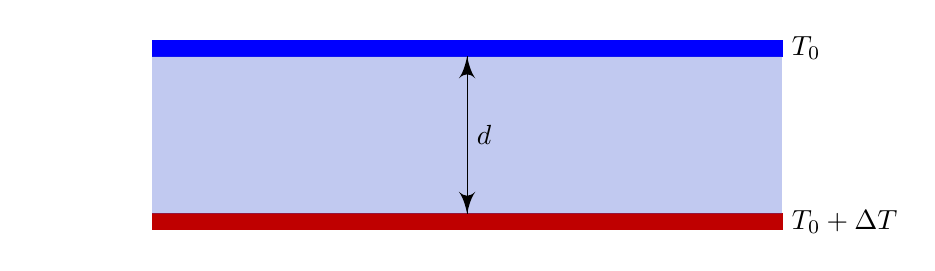
\begin{tikzpicture}
    \draw [red!50!mred, fill] (0, 0) rectangle (8, -0.2);
    \draw [blue, fill] (0, 2) rectangle (8, 2.2);

    \fill [mblue, opacity=0.3] (0, 0) rectangle (8, 2);

    \node [right] at (8, 2.1) {$T_0$};
    \node [right] at (8, -0.1) {$T_0 + \Delta T$};
    \node [white, left] at (0, -0.1) {$T_0 + \Delta T$};

    \draw [<->] (4, 0) -- (4, 2) node [pos=0.5, right] {$d$};
  \end{tikzpicture}
\end{center}
There is a hot plate at the bottom, a cold plate on top, and some fluid in between. We would naturally expect heat to transmit from the bottom to the top. There are two ways this can happen:
\begin{itemize}
  \item Conduction: Heat simply diffuses from the bottom to the top, without any fluid motion.
  \item Convection: The fluid at the bottom heats up, expands, becomes lighter, and moves to the top.
\end{itemize}
The first factor is controlled purely by thermal diffusivity $\kappa$, while the latter is mostly controlled by the viscosity $\nu$. It is natural to expect that when the temperature gradient $\Delta T$ is small, most of the heat transfer is due to conduction, as there isn't enough force to overcome the viscosity to move fluid around. When $\Delta T$ is large, the heat transfer will be mostly due to conduction, and we would expect such a system to be unstable.

To understand the system mathematically, we must honestly deal with the case where we have density variations throughout the fluid. Again, recall that the Navier--Stokes equation
\[
  \rho\left(\frac{\partial \mathbf{u}}{\partial t} + \mathbf{u} \cdot \nabla \mathbf{u}\right) = - \nabla P- g \rho \hat{\mathbf{z}} + \mu \nabla^2 \mathbf{u},\quad \nabla \cdot \mathbf{u} = 0.
\]
The static solution to our system is the pure conduction solution, where $\mathbf{u} = 0$, and there is a uniform vertical temperature gradient across the fluid. Since the density is a function of temperature, which in the static case is just a function of $z$, we know $\rho = \rho(z)$. When we perturb the system, we allow some horizontal and time-dependent fluctuations, and assume we can decompose our density field into
\[
  \rho = \rho_h(z) + \rho'(x, t).
\]
We can then define the hydrostatic pressure by the equation
\[
  \frac{\d P_h}{\d z} = - g\rho_h.
\]
This then allows us to decompose the pressure as
\[
  P = P_h(z) + p'(x, t).
\]
Then our equations of motion become
\[
  \frac{\partial \mathbf{u}}{\partial t} + \mathbf{u} \cdot \nabla \mathbf{u} = - \frac{1}{\rho} \nabla p' - \frac{g\rho'}{\rho} \hat{\mathbf{z}} + \nu \nabla^2 \mathbf{u},\quad \nabla \cdot \mathbf{u} = 0
\]
We have effectively ``integrated out'' the hydrostatic part, and it is now the deviation from the average that leads to buoyancy forces.

An important component of our analysis involves looking at the vorticity. Indeed, vorticity necessarily arises if we have non-trivial density variations. For concreteness, suppose we have a interface between two fluids with different densities, $\rho$ and $\rho + \Delta \rho$. If the interface is horizontal, then nothing happens:

\begin{center}
  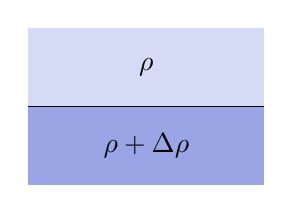
\begin{tikzpicture}
    \fill [mblue, opacity=0.5] (0, 0) rectangle (3, -1);
    \fill [mblue, opacity=0.2] (0, 0) rectangle (3, 1);

    \draw (0, 0) -- (3, 0);
    \node at (1.5, 0.5) {$\rho$};
    \node at (1.5, -0.5) {$\rho + \Delta \rho$};

  \end{tikzpicture}
\end{center}
However, if the interface is tilted, then there is a naturally induced torque:
\begin{center}
  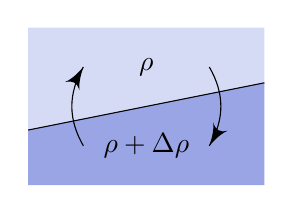
\begin{tikzpicture}
    \fill [mblue, opacity=0.5] (0, -0.3) -- (3, 0.3) -- (3, -1) -- (0, -1);
    \fill [mblue, opacity=0.2] (0, -0.3) -- (3, 0.3) -- (3, 1) -- (0, 1);

    \draw (0, -0.3) -- (3, 0.3);
    \node at (1.5, 0.5) {$\rho$};
    \node at (1.5, -0.5) {$\rho + \Delta \rho$};

    \draw (0.7, -0.5) edge [out=120, in=240, ->] (0.7, 0.5);
    \draw (2.3, 0.5) edge [out=300, in=60, ->] (2.3, -0.5);
  \end{tikzpicture}
\end{center}
In other words, \emph{vorticity} is induced. If we think about it, we see that the reason this happens is that the direction of the density gradient does not align with the direction of gravity. More precisely, this is because the density gradient does not align with the pressure gradient.

Let's try to see this from our equations. Recall that the vorticity is defined by\index{vorticity}\index{$\boldsymbol\omega$}
\[
  \boldsymbol\omega = \nabla \times \mathbf{u}.
\]
Taking the curl of the Navier--Stokes equation, and doing some vector calculus, we obtain the equation.
\[
  \frac{\partial \boldsymbol\omega}{\partial t} + \mathbf{u} \cdot \nabla \boldsymbol\omega = \boldsymbol\omega \cdot \nabla \mathbf{u} + \frac{1}{\rho^2}\nabla \rho \times \nabla P + \nu \nabla^2 \boldsymbol\omega
\]
The term on the left hand side is just the material derivative of the vorticity. So we should interpret the terms on the right-hand-side as the terms that contribute to the change in vorticity.

The first and last terms on the right are familiar terms that have nothing to do with the density gradient. The interesting term is the second one. This is what we just described --- whenever the pressure gradient and density gradient do not align, we have a \term{baroclinic torque}. % describe other terms as well.

%The left hand side is just the change in vorticity along the flow. The first term on the left is describing what happens when we stretch a vortex, which by conservation of momentum implies that the spin increases. The second term is what we just described --- if the pressure gradient points differently from the density gradient, then we get a torque, called \term{baroclinic torque}.

In general, equations are hard to solve, and we want to make approximations. A common approximation is the \term{Boussinesq approximation}. The idea is that even though the density difference is often what drives the motion, from the point of view of inertia, the variation in density is often small enough to be ignored. To take some actual, physical examples, salt water is roughly $4\%$ more dense than fresh water, and every $10$ degrees Celsius changes the density of air by approximately $4\%$.

Thus, what we do is that we assume that the density is constant except in the buoyancy force. The mathematically inclined people could think of this as taking the limit $g \to \infty$ but $\rho' \to 0$ with $g \rho'$ remaining finite.

Under this approximation, we can write our equations as
\begin{align*}
  \frac{\partial \mathbf{u}}{\partial t} + \mathbf{u}\cdot \nabla \mathbf{u} &= - \frac{1}{\rho_0} \nabla p' - g' \hat{\mathbf{z}} + \nu \nabla^2 \mathbf{u}\\
  \frac{\partial \boldsymbol\omega}{\partial t} + \mathbf{u} \cdot \nabla\boldsymbol\omega &= \boldsymbol\omega \cdot \nabla \mathbf{u} + \frac{g}{\rho_0} \hat{\mathbf{z}} \times \nabla \rho + \nu \nabla^2 \boldsymbol\omega,
\end{align*}
where we define the \term{reduced gravity} to be
\[
  g' = \frac{g \rho'}{\rho_0}
\]
Recall that our density is to be given by a function of temperature $T$. We must write down how we want the two to be related. In reality, this relation is extremely complicated, and may be affected by other external factors such as salinity (in the sea). However, we will use a ``leading-order'' approximation
\[
  \rho = \rho_0 (1 - \alpha(T - T_0)).
\]
We will also need to know how temperature $T$ evolves in time. This is simply given by the diffusion equation
\[
  \frac{\partial T}{\partial t} + \mathbf{u} \cdot \nabla T = \kappa \nabla^2 T.
\]
Note that in thermodynamics, temperature and pressure are related quantities. In our model, we will completely forget about this. The only purpose of pressure will be to act as a non-local Lagrange multiplier that enforces incompressibility.

There are some subtleties with this approximation. Inverting the relation,
\[
  T = \frac{1}{\alpha}\left(1 - \frac{\rho}{\rho_0}\right) + T_0.
\]
Plugging this into the diffusion equation, we obtain
\[
  \frac{\partial \rho}{\partial t} + \mathbf{u} \cdot \nabla \rho = \kappa \nabla^2 \rho.
\]
The left-hand side is the material derivative of density. So this equation is saying that density, or mass, can ``diffuse'' along the fluid, independent of fluid motion. Mathematically, this follows from the fact that density is directly related to temperature, and temperature diffuses.

This seems to contradict the conservation of mass. Recall that the conservation of mass says
\[
  \frac{\partial \rho}{\partial t} + \nabla \cdot (\mathbf{u} \rho) = 0.
\]
We can than expand this to say
\[
  \frac{\partial \rho}{\partial t} + \mathbf{u} \cdot \nabla \rho = - \rho \nabla \cdot \mathbf{u}.
\]
We just saw that the left-hand side is given by $\kappa \nabla^2 \rho$, which can certainly be non-zero, but the right-hand side should vanish by incompressibility! The issue is that here the change in $\rho$ is not due to compressing the fluid, but simply thermal diffusion.

If we are not careful, we may run into inconsistencies if we require $\nabla \cdot \mathbf{u} = 0$. For our purposes, we will not worry about this too much, as we will not use the conservation of mass.

We can now return to our original problem. We have a fluid of viscosity $\nu$ and thermal diffusivity $\kappa$. There are two plates a distance $d$ apart, with the top held at temperature $T_0$ and bottom at $T_0 + \Delta T$. We make the Boussinesq approximation.
\begin{center}
  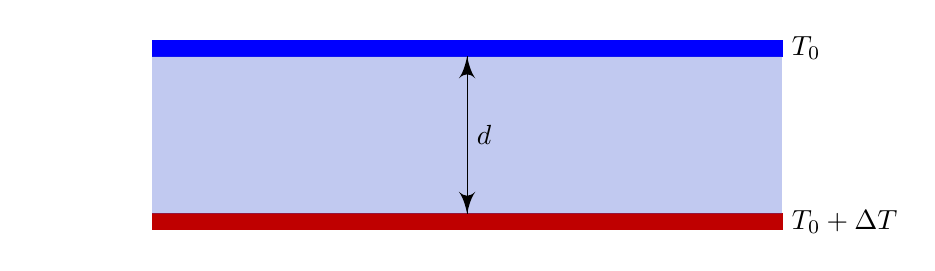
\begin{tikzpicture}
    \draw [red!50!mred, fill] (0, 0) rectangle (8, -0.2);
    \draw [blue, fill] (0, 2) rectangle (8, 2.2);

    \fill [mblue, opacity=0.3] (0, 0) rectangle (8, 2);

    \node [right] at (8, 2.1) {$T_0$};
    \node [right] at (8, -0.1) {$T_0 + \Delta T$};
    \node [white, left] at (0, -0.1) {$T_0 + \Delta T$};

    \draw [<->] (4, 0) -- (4, 2) node [pos=0.5, right] {$d$};
  \end{tikzpicture}
\end{center}
We first solve for our steady state, which is simply
\begin{align*}
  \mathbf{U} &= \mathbf{0}\\
 T_h &= T_0 - \Delta T \frac{(z - d)}{d}\\
 \rho_h &= \rho_0 \left(1 + \alpha \Delta T \frac{z - d}{d}\right)\\
 P_h &= P_0 - g \rho_0 \left(z + \frac{\alpha \Delta Tz}{2d}(z - 2d)\right),
\end{align*}
In this state, the only mode of heat transfer is conduction. What we would like to investigate, of course, is whether this state is stable. Consider small perturbations
\begin{align*}
  \mathbf{u} &= \mathbf{U} + \mathbf{u}'\\
  T &= T_h + \theta\\
  P &= P_h + p'.
\end{align*}
We substitute these into the Navier--Stokes equation. Starting with
\[
  \frac{\partial \mathbf{u}}{\partial t} + \mathbf{u} \cdot \nabla \mathbf{u} = -\frac{1}{\rho_0} \nabla p' + g \alpha \theta \hat{\mathbf{z}} + \nu \nabla^2 \mathbf{u},
\]
we assume the term $\mathbf{u} \cdot \nabla \mathbf{u}$ will be small, and end up with the equation
\[
  \frac{\partial \mathbf{u}'}{\partial t} = - \frac{1}{\rho_0} \nabla p' + g \alpha \theta \hat{\mathbf{z}} + \nu \nabla^2 \mathbf{u},
\]
together with the incompressibility condition $\nabla \cdot \mathbf{u}' = 0$.

Similarly, plugging these into the temperature diffusion equation and writing $\mathbf{u} = (u, v, w)$ gives us
\[
  \frac{\partial \theta}{\partial t} - w' \frac{\Delta T}{d} = \kappa \nabla^2 \theta.
\]
We can gain further understanding of these equations by expressing them in terms of dimensionless quantities. We introduce new variables
\begin{align*}
  \tilde{t} &= \frac{\kappa t}{d^2} & \tilde{\mathbf{x}} &= \frac{\mathbf{x}}{d}\\
  \tilde{\theta} &= \frac{\theta}{\Delta T} & \tilde{p} &= \frac{d^2 p'}{\rho_0 \kappa^2}
\end{align*}
In terms of these new variables, our equations of motion become rather elegant:
\begin{align*}
  \frac{\partial \tilde{\theta}}{\partial \tilde{t}} - \tilde{w} &= \tilde{\nabla}^2 \tilde{\theta}\\
  \frac{\partial \tilde{\mathbf{u}}}{\partial \tilde{t}} &= - \tilde{\nabla} \tilde{p} + \left(\frac{g\alpha \Delta T d^3}{\nu\kappa}\right) \left(\frac{\nu}{\kappa}\right) \tilde{\theta} \hat{\mathbf{z}} + \frac{\nu}{\kappa} \tilde{\nabla}^2 \tilde{\mathbf{u}}
\end{align*}
Ultimately, we see that the equations of motion depend on two dimensionless constants: the \term{Rayleigh number} and \term{Prandtl number}
\begin{align*}
  \Ra &= \frac{g\alpha \Delta T d^3}{\nu\kappa}\\
  \Pr &= \frac{\nu}{\kappa},
\end{align*}
These are the two parameters control the behaviour of the system. In particular, the Prandtl number measures exactly the competition between viscous and diffusion forces. Different fluids have different Prandtl numbers:
\begin{itemize}
  \item In a gas, then $\frac{\nu}{\kappa} \sim 1$, since both are affected by the mean free path of a particle.
  \item In a non-metallic liquid, the diffusion of heat is usually much slower than that of momentum, so $\Pr \sim 10$.
  \item In a liquid metal, $\Pr$ is very very low, since, as we know, metal transmits heat quite well.
\end{itemize}
Finally, the incompressibility equation still reads
\[
  \tilde{\nabla} \cdot \tilde{\mathbf{u}} = 0
\]
Under what situations do we expect an unstable flow? Let's start with some rather more heuristic analysis. Suppose we try to overturn our system as shown in the diagram:
\begin{center}
  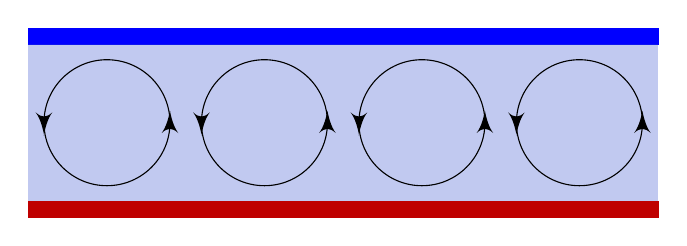
\begin{tikzpicture}
    \draw [red!50!mred, fill] (0, 0) rectangle (8, -0.2);
    \draw [blue, fill] (0, 2) rectangle (8, 2.2);

    \fill [mblue, opacity=0.3] (0, 0) rectangle (8, 2);

    \foreach \x in {0,2,4,6} {
      \begin{scope}[shift={(\x, 0)}]
        \draw (1, 1) circle [radius=0.8];
        \draw [->] (0.2, 0.85) -- +(0, -0.0001);
        \draw [->] (1.8, 1.15) -- +(0, 0.0001);
      \end{scope}
    }
  \end{tikzpicture}
\end{center}

Suppose we do this at a speed $U$. For each $d \times d \times d$ block, the potential energy released is
\[
  PE \sim g \cdot d \cdot (d^3 \Delta \rho) \sim g \rho_0 \alpha d^4 \Delta T,
\]
and the time scale for this to happen is $\tau \sim d/U$.

What is the friction we have to overcome in order to achieve this? The viscous stress is approximately
\[
  \mu \frac{\partial U}{\partial z} \sim \mu \frac{U}{d}.
\]
The force is the integral over the area, which is $\sim \frac{\mu U}{d} d^2$. The work done, being $\int F \;\d z$, then evaluates to
\[
  \frac{\mu U}{d} \cdot d^2 \cdot d = \mu U d^2.
\]
We can figure out $U$ by noting that the heat is diffused away on a time scale of $\tau \sim d^2 / \kappa$. For convection to happen, it must occur on a time scale at least as fast as that of diffusion. So we have $U \sim \kappa/d$. All in all, for convection to happen, we need the potential energy gain to be greater than the work done, which amounts to
\[
  g \rho_0 \alpha \Delta T d^4 \gtrsim \rho_0 \nu \kappa d.
\]
In other words, we have
\[
  \Ra = \frac{g \alpha \Delta T d^3}{\nu \kappa} = \frac{g' d^3}{\nu \kappa} \gtrsim 1.
\]
Now it is extremely unlikely that $\Ra \geq 1$ is indeed the correct condition, as our analysis was not very precise. However, it is generally true that instability occurs only when $\Ra$ is large.

To work this out, let's take the curl of the Navier--Stokes equation we previously obtained, and dropping the tildes, we get
\[
 \frac{\partial \boldsymbol\omega}{\partial t} = \Ra \Pr \nabla \theta \times \hat{\mathbf{z}} + \Pr \nabla^2 \boldsymbol\omega
\]
This gets rid of the pressure term, so that's one less thing to worry about. But this is quite messy, so we take the curl yet again to obtain
\[
 \frac{\partial}{\partial t} \nabla^2 \mathbf{u} = \Ra \Pr \left(\nabla^2 \theta \hat{\mathbf{z}} - \nabla \left(\frac{\partial \theta}{\partial z}\right)\right) + \Pr \nabla^4 \mathbf{u}
\]
Reading off the $z$ component, we get
\[
  \frac{\partial}{\partial t} \nabla^2 w = \Ra \Pr \left(\frac{\partial^2}{\partial x^2} + \frac{\partial^2}{\partial y^2}\right) \theta + \Pr \nabla^4 w.
\]
We will combine this with the temperature equation
\[
  \frac{\partial \theta}{\partial t} - w = \nabla^2 \theta
\]
to understand the stability problem.

We first try to figure out what boundary conditions to impose. We've got a $6$th order partial differential equation ($4$ from the Navier--Stokes and $2$ from the temperature equation), and so we need $6$ boundary conditions. It is reasonable to impose that $w = \theta = 0$ at $z = 0, 1$, as this gives us impermeable boundaries.

It is also \emph{convenient} to assume the top and bottom surfaces are stress-free: $\frac{\partial u}{\partial z} = \frac{\partial v}{\partial z} = 0$, which implies
\[
  \frac{\partial}{\partial z} \left(\frac{\partial u}{\partial x} + \frac{\partial v}{\partial y}\right) = 0.
\]
This then gives us $\frac{\partial^2 w}{\partial z^2} = 0$. This is does \emph{not} make much physical sense, because our fluid is viscous, and we should expect no-slip boundary conditions, not no-stress. But they are mathematically convenient, and we shall assume them.

Let's try to look for unstable solutions using separation of variables. We see that the equations are symmetric in $x$ and $y$, and so we write our solution as
\begin{align*}
  w &= W(z) X(x, y) e^{\sigma t}\\
  \theta &= \Theta(z) X(x, y) e^{\sigma t}.
\end{align*}
If we can find solutions of this form with $\sigma > 0$, then the system is unstable.

What follows is just a classic separation of variables. Plugging these into the temperature equation yields
\[
  \left(\frac{\d^2}{\d z^2} - \sigma + \left(\frac{\partial^2}{\partial x^2} + \frac{\partial^2}{\partial y^2}\right)\right) X \Theta = -XW.
\]
Or equivalently
\[
  \left(\frac{\d^2}{\d z^2} - \sigma\right) X\Theta + XW = - \left(\frac{\partial^2}{\partial x^2} + \frac{\partial^2}{\partial y^2}\right) X\Theta.
\]
We see that the differential operator on the left only acts in $\Theta$, while those on the right only act on $X$. We divide both sides by $X\Theta$ to get
\[
  \frac{\left(\frac{\d^2}{\d y^2} - \sigma\right) \Theta + W}{\Theta} = - \frac{\left(\frac{\d^2}{\d x^2} + \frac{\d^2}{\d y^2}\right) X}{X}.
\]
Since the LHS is purely a function of $z$, and the RHS is purely a function of $X$, they must be constant, and by requiring that the solution is bounded, we see that this constant must be positive. Our equations then become
\begin{align*}
  \left(\frac{\partial^2}{\partial x^2} + \frac{\partial^2}{\partial y^2} \right)X = - \lambda^2 X\\
  \left(\frac{\d^2}{\d z^2} - \lambda^2 - \sigma\right) \Theta = - W.
\end{align*}
We now look at our other equation. Plugging in our expressions for $w$ and $\theta$, and using what we just obtained, we have
\[
  \sigma\left(\frac{\d^2}{\d z^2} - \lambda^2 \right)W = - \Ra \Pr \lambda^2 \Theta + \Pr \left(\frac{\d^2}{\d z^2} - \lambda^2\right)^2 W.
\]
On the boundary, we have $\Theta = 0 = W = \frac{\partial^2 W}{\partial z^2} = 0$, by assumption. So it follows that we must have
\[
  \left.\frac{\d^4W}{\d z^4} \right|_{z = 0, 1} = 0.
\]
We can eliminate $\Theta$ by letting $\left(\frac{\d^2}{\d z^2} - \sigma - \lambda^2\right)$ act on both sides, which converts the $\Theta$ into $W$. We are then left with a $6$th order differential equation
\[
  \left(\frac{\d^2}{\d z^2} - \sigma - \lambda^2\right) \left(\Pr \left(\frac{\d^2}{\d z^2} - \lambda^2\right)^2 - \sigma \left(\frac{\d^2}{\d z^2} - \lambda^2\right)\right) W =- \Ra \Pr \lambda^2 W.
\]
This is an eigenvalue problem, and we see that our operator is self-adjoint. We can factorize and divide across by $\Pr$ to obtain
\[
  \left(\frac{\d^2}{\d z^2} - \lambda^2 \right) \left(\frac{\d^2}{\d z^2} - \sigma - \lambda^2\right) \left(\frac{\d^2}{\d z^2} - \lambda ^2 - \frac{\sigma}{\Pr}\right) W = - \Ra \lambda^2 W.
\]
The boundary conditions are that
\[
  W= \frac{\d^2 W}{\d z^2}= \frac{\d^4 W}{\d x^4} = 0\text{ at }z = 0, 1.
\]
We see that any eigenfunction of $\frac{\d^2}{\d z^2}$ gives us an eigenfunction of our big scary differential operator, and our solutions are quantized sine functions, $W = \sin n \pi z$ with $n \in \N$. In this case, the eigenvalue equation is
\[
  (n^2 \pi^2 + \lambda^2) (n^2 \pi^2 + \sigma + \lambda^2) \left(n^2\pi^2 + \lambda^2 + \frac{\sigma}{\Pr}\right) = \Ra \lambda^2.
\]
When $\sigma > 0$, then, noting that the LHS is increasing with $\sigma$ on the range $[0, \infty)$, this tells us that we have
\[
  \Ra(n) \geq \frac{(n^2 \pi^2 + \lambda^2)^3}{\lambda^2}.
\]
We minimize the RHS with respect to $\lambda$ and $n$. We clearly want to set $n = 1$, and then solve for
\[
  0 = \frac{\d}{\d [\lambda^2]} \frac{(n^2 \pi^2 + \lambda^2)^3}{\lambda^2} = \frac{(\pi^2 + \lambda^2)^2}{\lambda^4}(2\lambda^2 - \pi^2).
\]
So the minimum value of $\Ra$ is obtained when
\[
  \lambda_c = \frac{\pi}{\sqrt{2}}.
\]
So we find that we have a solution only when
\[
  \Ra \geq \Ra_c = \frac{27\pi^4}{4} \approx 657.5.
\]
If we are slightly about $\Ra_c$, then there is the $n = 1$ unstable mode. As $\Ra$ increases, the number of available modes increases. While the critical Rayleigh number depends on boundary conditions, but the picture is generic, and the width of the unstable range grows like $\sqrt{\Ra - \Ra_c}$:
\begin{center}
  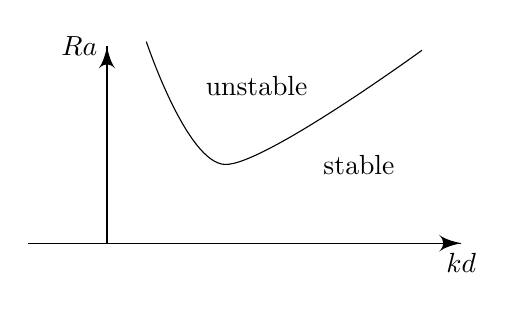
\begin{tikzpicture}
    \draw [->] (-1, 0) -- (4.5, 0) node [below] {$kd$};

    \draw [->] (0, 0) -- (0, 2.5) node [left] {$Ra$};

    \draw plot [smooth] coordinates {(0.5, 2.56) (1.5, 1) (4, 2.45)};

    \node at (3.2, 1) {stable};
    \node at (1.9, 2) {unstable};
  \end{tikzpicture}
\end{center}

We might ask --- how does convection enhance the heat flux? This is quantified by the \term{Nusselt number}
\[
  Nu = \frac{\text{convective heat transfer}}{\text{conductive heat transfer}} = \frac{\bra wT\ket d}{\kappa \Delta T} = \bra \tilde{w} \tilde{\theta}\ket.
\]
Since this is a non-dimensional number, we know it is a function of $\Ra$ and $\Pr$.

There are some physical arguments we can make about the value of $Nu$. The claim is that the convective heat transfer is independent of layer depth. If there is no convection at all, then the temperature gradient will look approximately like

There is some simple arguments we can make about this. If we have a purely conductive state, then we expect the temperature gradient to be linear:
\begin{center}
  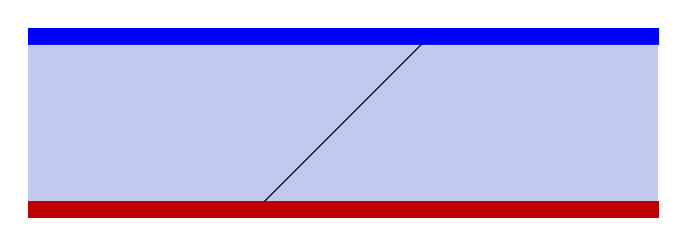
\begin{tikzpicture}
    \draw [red!50!mred, fill] (0, 0) rectangle (8, -0.2);
    \draw [blue, fill] (0, 2) rectangle (8, 2.2);

    \fill [mblue, opacity=0.3] (0, 0) rectangle (8, 2);

    \draw (3, 0) -- (5, 2);
  \end{tikzpicture}
\end{center}
This is pretty boring. If there is convection, then we claim that the temperature gradient will look like
\begin{center}
  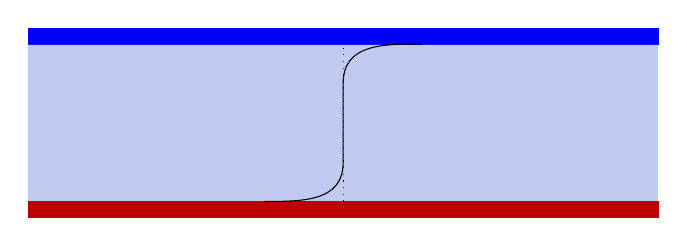
\begin{tikzpicture}
    \draw [red!50!mred, fill] (0, 0) rectangle (8, -0.2);
    \draw [blue, fill] (0, 2) rectangle (8, 2.2);

    \fill [mblue, opacity=0.3] (0, 0) rectangle (8, 2);

    \draw [dotted] (4, 0) -- (4, 2);

    \draw (3, 0) .. controls (3.5, 0) and (4, 0) .. (4, 0.5) -- (4, 1.5) .. controls (4, 2) and (4.5, 2) .. (5, 2);
  \end{tikzpicture}
\end{center}
The reasoning is that the way convection works is that once a parcel at the bottom is heated to a sufficiently high temperature, it gets kicked over to the other side; if a parcel at the top is cooled to a sufficiently low temperature, it gets kicked over to the other side. In between the two boundaries, the temperature is roughly constant, taking the average temperature of the two boundaries.

In this model, it doesn't matter how far apart the two boundaries are, since once the hot or cold parcels are shot off, they can just travel on their own until they reach the other side (or mix with the fluid in the middle).

If we believe this, then we must have $\bra wT \ket \propto d^0$, and hence $Nu \propto d$. Since only $\Ra$ depends on $d$, we must have $Nu \propto \Ra^{1/3}$.

Of course, the real situation is much more subtle.

\subsection{Classical Kelvin--Helmholtz instability}
Let's return to the situation of Rayleigh--Taylor instability, but this time, there is some horizontal flow in the two layers, and they may be of different velocities.
\begin{center}
  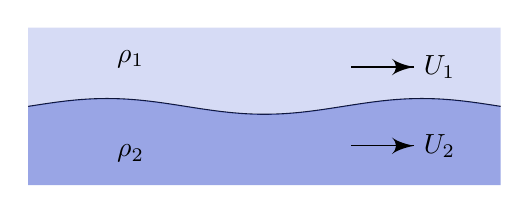
\begin{tikzpicture}
    \draw (-3, 0) sin (-2, 0.1) cos (-1, 0) sin (0, -0.1) cos (1, 0) sin (2, 0.1) cos (3, 0);
    \fill [mblue, opacity=0.5] (-3, -1) -- (-3, 0) sin (-2, 0.1) cos (-1, 0) sin (0, -0.1) cos (1, 0) sin (2, 0.1) cos (3, 0) -- (3, -1);
    \fill [mblue, opacity=0.2] (-3, 1) -- (-3, 0) sin (-2, 0.1) cos (-1, 0) sin (0, -0.1) cos (1, 0) sin (2, 0.1) cos (3, 0) -- (3, 1);

    \node at (-1.7, -0.6) {$\rho_2$};
    \node at (-1.7, 0.6) {$\rho_1$};

    \draw [->] (1.1, 0.5) -- (1.9, 0.5) node [right] {$U_1$};
    \draw [->] (1.1, -0.5) -- (1.9, -0.5) node [right] {$U_2$};
  \end{tikzpicture}
\end{center}

Our analysis here will be not be very detailed, partly because what we do is largely the same as the analysis of the Rayleigh--Taylor instability, but also because the analysis makes quite a few assumptions which we wish to examine more deeply.

In this scenario, we can still use a velocity potential
\[
  (u, w) = \left(\frac{\partial \phi}{\partial x}, \frac{\partial \phi}{\partial z}\right).
\]
We shall only consider the system in $2D$. The far field now has velocity
\begin{align*}
  \phi_1 &= U_1 x + \phi_1'\\
  \phi_2 &= U_2 x + \phi_2'
\end{align*}
with $\phi_1' \to 0$ as $z \to \infty$ and $\phi_2' \to 0$ as $z \to -\infty$.

The boundary conditions are the same. Continuity of vertical velocity requires
\[
  \left.\frac{\partial \phi_{1, 2}}{\partial z} \right|_{z = \eta} = \frac{\D \eta}{\D t}.
\]
The dynamic boundary condition is that we have continuity of pressure at the interface if there is no surface tension, in which case Bernoulli tells us
\[
  \rho_1 \frac{\partial \phi_1}{\partial t} + \frac{1}{2} \rho_1 |\nabla \phi_1|^2 + g \rho_1 \eta = \rho_2 \frac{\partial \phi_2}{\partial t} + \frac{1}{2} \rho_2 |\nabla \phi_2|^2 + g \rho_2 \eta.
\]
The interface conditions are non-linear, and again we want to linearize. But since $U_{1, 2}$ is of order $1$, linearization will be different. We have
\[
  \left. \frac{\partial \phi'_{1, 2}}{\partial z} \right|_{z = 0} = \left(\frac{\partial}{\partial t} + U_{1, 2} \frac{\partial}{\partial x}\right)\eta.
\]
So the Bernoulli condition gives us
\[
  \rho_1 \left(\left(\frac{\partial}{\partial t} + U_1 \frac{\partial}{\partial x}\right) \phi_1' + g \eta\right) = \rho_2 \left(\left(\frac{\partial}{\partial t} + U_2 \frac{\partial}{\partial x}\right) \phi_2' + g \eta\right)
\]
This modifies our previous eigenvalue problem for the phase speed and wavenumber $\omega = k c$, $k = \frac{2\pi}{\lambda}$. We go exactly as before, and after some work, we find that we have
\[
  c = \frac{\rho_1 U_1 + \rho_2 U_2}{\rho_1 + \rho_2} \pm \frac{1}{\rho_1 + \rho_2} \left(\frac{g (\rho_2^2 - \rho_1^2)}{k} - \rho_1 \rho_2 (U_1 - U_2)^2\right)^{1/2}.
\]
So we see that we have instability if $c$ has an imaginary part, i.e.
\[
  k > \frac{g (\rho_2^2 - \rho_1^2)}{\rho_1 \rho_2 (U_1 - U_2)^2}.
\]
So we see that there is instability for sufficiently large wavenumbers, even for static stability. Similar to Rayleigh--Taylor instability, the growth rate $k c_i$ grows monotonically with wavenumber, and as $k \to \infty$, the instability becomes proportional to the difference $|U_1 - U_2|$ (as opposed to Rayleigh--Taylor instability, where it grows unboundedly). % c_i and c_r are real and imaginary components of c

How can we think about this result? If $U_1 \not= U_2$ and we have a discrete change in velocity, then this means there is a $\delta$-function of vorticity at the interface. So it should not be surprising that the result is unstable!

Another way to think about it is to change our frame of reference so that $U_1 = U = - U_2$. In the Boussinesq limit, we have $c_r = 0$, and instability arises whenever $\frac{g \Delta \rho \lambda}{\rho U^2} < 4\pi$. We can see the numerator as the potential energy cost if we move a parcel from the bottom layer to the top layer, while the denominator as some sort of kinetic energy. So this says we are unstable if there is enough kinetic energy to move a parcel up.

This analysis of the shear flow begs a few questions:
\begin{itemize}
  \item How might we regularize this expression? The vortex sheet is obviously wildly unstable.
  \item Was it right to assume two-dimensional perturbations?
  \item What happens if we regularize the depth of the shear?
\end{itemize}

\subsection{Finite depth shear flow}
We now consider a finite depth shear flow. This means we have fluid moving between two layers, with a $z$-dependent velocity profile:
\begin{center}
  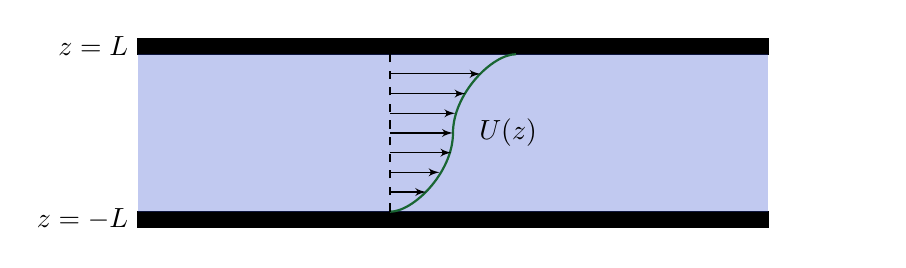
\begin{tikzpicture}
    \draw [black, fill] (0, 0) rectangle (8, -0.2);
    \draw [black, fill] (0, 2) rectangle (8, 2.2);

    \fill [mblue, opacity=0.3] (0, 0) rectangle (8, 2);

    \node [left] at (0, 2.1) {$z = L$};
    \node [left] at (0, -0.1) {$z = -L$};
    \node [white, right] at (8, -0.1) {$z = -L$};

    \draw [thick, mgreen] (3.2, 0) .. controls (3.5, 0) and (4, 0.5) .. (4, 1) .. controls (4, 1.5) and (4.5, 2) .. (4.8, 2);
    \draw [dashed] (3.2, 0) -- ++(0, 2);

    \draw [-latex'] (3.2, 0.25) -- +(0.46, 0);
    \draw [-latex'] (3.2, 0.50) -- +(0.63, 0);
    \draw [-latex'] (3.2, 0.75) -- +(0.78, 0);
    \draw [-latex'] (3.2, 1.00) -- +(0.8, 0);
    \draw [-latex'] (3.2, 1.25) -- +(0.83, 0);
    \draw [-latex'] (3.2, 1.50) -- +(0.96, 0);
    \draw [-latex'] (3.2, 1.75) -- +(1.15, 0);

    \node at (4.7, 1) {$U(z)$};
  \end{tikzpicture}
\end{center}
We first show that it suffices to work in $2$ dimensions. We will assume that the mean flow points in the $\hat{\mathbf{x}}$ direction, but the perturbations can point at an angle. The inviscid homogeneous incompressible Navier--Stokes equations are again
\[
  \left(\frac{\partial \mathbf{u}}{\partial t} + \mathbf{u} \cdot \nabla \mathbf{u}\right) = \frac{\D \mathbf{u}}{\D t} = - \nabla \left(\frac{p'}{\rho}\right),\quad \nabla \cdot \mathbf{u} = 0.
\]
We linearize about a shear flow, and consider some 3D normal modes
\[
  \mathbf{u} = \bar{U}(z)\hat{\mathbf{x}} + \mathbf{u}'(x, y, z, t),
\]
where
\[
  (\mathbf{u}', p'/\rho) = [\hat{\mathbf{u}}(z), \hat{p}(z)]e^{i (kx + \ell y - kct)}.
\]
The phase speed is then
\[
  c_p = \frac{\omega}{\kappa} = \frac{\omega}{(k^2 + \ell^2)^{1/2}} = \frac{kc_r}{(k^2 + \ell^2)^{1/2}}
\]
and the growth rate of the perturbation is simply $\sigma_{3d} = k c_i$.

We substitute our expression of $\mathbf{u}$ and $p'/\rho$ into the Navier--Stokes equations to obtain, in components,
\begin{align*}
  ik (\bar{U} - c) \hat{u} + \hat{w} \frac{\d \bar{U}}{\d z} &= - ik \hat{p}\\
  ik (\bar{U} - c) \hat{v} &= - il \hat{p}\\
  ik (\bar{U} - c) \hat{w} &= - \frac{\d \hat{p}}{\d z}\\
  ik \hat{u} + i\ell\hat{v} + \frac{\d\hat{w}}{\d z} &= 0
\end{align*}
Our strategy is to rewrite everything to express things in terms of new variables
\[
  \kappa = \sqrt{k^2 + \ell^2},\quad \kappa \tilde{u} = k\hat{u} + \ell\hat{v},\quad \tilde{p} = \frac{\kappa \hat{p}}{k}
\]
and if we are successful in expressing everything in terms of $\tilde{u}$, then we could see how we can reduce this to the two-dimensional problem.

To this end, we can slightly rearrange our first two equations to say
\begin{align*}
  ik (\bar{U} - c) \hat{u} + \hat{w} \frac{\d \bar{U}}{\d z} &= - ik^2 \frac{\hat{p}}{k}\\
  i\ell (\bar{U} - c) \hat{v} &= - i\ell^2 \frac{\hat{p}}{k}
\end{align*}
which combine to give
\[
  i (\bar{U} - c) \kappa \tilde{u} + \hat{w} \frac{\d \bar{U}}{\d z} = - i \kappa \tilde{p}.
\]
We can rewrite the remaining two equations in terms of $\tilde{p}$ as well:
\begin{align*}
  i \kappa (\bar{U} - c) \hat{w} &= - \frac{\d}{\d z} \tilde{p}\\
  \kappa \tilde{U} + \frac{\d \hat{w}}{\d z} &= 0.
\end{align*}
This looks just like a 2d system, but with an instability growth rate of $\sigma_{2d} = \kappa c_i > k c_i = \sigma_{3d}$. Thus, our 3d problem is ``equivalent'' to a 2d problem with greater growth rate. However, whether or not instability occurs is unaffected. One way to think about the difference in growth rate is that the $y$ component of the perturbation sees less of the original velocity $\bar{U}$, and so it is more stable. This result is known as \term{Squire's Theorem}.

We now restrict to two-dimensional flows, and have equations
\begin{align*}
  ik (\bar{U} - c) \hat{u} + \hat{w} \frac{\d \bar{U}}{\d z} &= ik\hat{p}\\
  ik (\bar{U} - c) \hat{w} &= - \frac{\d \hat{p}}{\d z}\\
  ik \hat{u} + \frac{\d \hat{w}}{\d z} &= 0.
\end{align*}
We can use the last incompressibility equation to eliminate $\hat{u}$ from the first equation, and be left with
\[
  -(\bar{U} - c) \frac{\d \hat{w}}{\d z} + \hat{w} \frac{\d \bar{U}}{\d z} = - ik \hat{p}.
\]
We wish to get rid of the $\hat{p}$, and to do so, we differentiate this equation with respect to $z$ and use the second equation to get
\[
  -(\bar{U} - c) \frac{\d^2 \hat{w}}{\d z^2} - \frac{\d \hat{w}}{\d z} \frac{\d \bar{U}}{\d z} + \frac{\d \hat{w}}{\d z} \frac{\d \bar{U}}{\d z} + \hat{w} \frac{\d^2 \bar{U}}{\d z^2} = -k^2 (\bar{U} - c) \hat{w}.
\]
The terms in the middle cancel, and we can rearrange to obtain the \term{Rayleigh equation}
\[
  \left((\bar{U} - c) \left(\frac{\d^2}{\d z^2} - k^2\right) - \frac{\d^2 \bar{U}}{\d z^2} \right) \hat{w} = 0.
\]
We see that when $\bar{U} = c$, we have a regular singular point. The natural boundary conditions are that $\hat{w} \to 0$ at the edge of the domain.

Note that this differential operator is not self-adjoint! This is since $\bar{U}$ has non-trivial $z$-dependence. This means we do not have a complete basis of orthogonal eigenfunctions. This is manifested by the fact that it can have transient growth.

To analyze this scenario further, we rewrite Rayleigh equation in conventional form
\[
  \frac{\d^2 \hat{w}}{\d z^2} - k^2 \hat{w} - \frac{\d^2 \bar{U}/\d z^2}{\bar{U} - c} \hat{w} = 0.
\]
The trick is to multiply by $w^*$, integrate across the domain, and apply boundary conditions to obtain
\[
  \int_{-L}^L \frac{\bar{U}''}{\bar{U} - c} |\hat{w}|^2 \;\d z = - \int_{-L}^L (|\hat{w}'|^2 + k^2 |\hat{w}|^2)\;\d z
\]
We can split the LHS into real and imaginary parts:
\[
  \int_{-L}^L \left( \frac{\bar{U}''(\bar{U} - c_r)}{|\bar{U} - c|^2}\right) |\hat{w}|^2 \;\d z + i c_i \int_{-L}^L \left(\frac{\bar{U}''}{ |\bar{U} - c|^2}\right) |\hat{w}|^2 \;\d z.
\]
But since the RHS is purely real, we know the imaginary part must vanish.

One way for the imaginary part to vanish is for $c_i$ to vanish, and this corresponds to stable flow. If we want $c_i$ to be non-zero, then the integral must vanish. So we obtain the \term{Rayleigh inflection point criterion}: $\frac{\d^2}{\d z^2} \bar{U}$ must change sign at least once in $-L < z < L$.

Of course, this condition is not sufficient for instability. If we want to get more necessary conditions for instability to occur, it might be wise to inspect the imaginary part, as Fjortoft noticed. If instability occurs, then we know that we must have
\[
  \int_{-L}^L \left(\frac{\bar{U}''}{|\bar{U} - c|^2} \right) |\hat{w}|^2\;\d z = 0.
\]
Let's assume that there is a unique (non-degenerate) inflection point at $z = z_s$, with $\bar{U}_s = \bar{U}(z_s)$. We can then add $(c_r - \bar{U}_s)$ times the above equation to the real part to see that we must have
\[
  -\int_{-L}^L (|\hat{w}'|^2 + k^2 |\hat{w}|^2)\;\d z = \int_{-L}^L \left(\frac{\bar{U}''(\bar{U} - \bar{U}_s)}{ |\bar{U} - c|^2} \right) |\hat{w}|^2\;\d z.
\]
Assuming further that $\bar{U}$ is monotonic, we see that both $\bar{U} - \bar{U}_s$ and $U''$ change sign at $z_s$, so the sign of the product is unchanged. So for the equation to be consistent, we must have $\bar{U}'' (\bar{U} - \bar{U}_s) \leq 0$ with equality only at $z_s$.

We can look at some examples of different flow profiles:
\begin{center}
  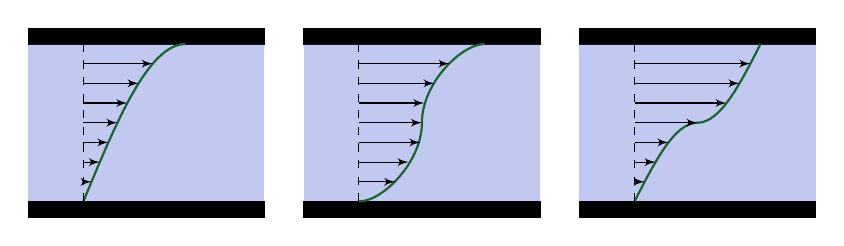
\begin{tikzpicture}
    \draw [black, fill] (-0.5, 0) rectangle (2.5, -0.2);
    \draw [black, fill] (-0.5, 2) rectangle (2.5, 2.2);

    \fill [mblue, opacity=0.3] (-0.5, 0) rectangle (2.5, 2);

    \draw [thick, mgreen] (0.2, 0) sin (1.5, 2);
    \draw [dashed] (0.2, 0) -- ++(0, 2);

    \draw [-latex'] (0.2, 0.25) -- +(0.1037, 0);
    \draw [-latex'] (0.2, 0.50) -- +(0.2091, 0);
    \draw [-latex'] (0.2, 0.75) -- +(0.3181, 0);
    \draw [-latex'] (0.2, 1.00) -- +(0.433, 0);
    \draw [-latex'] (0.2, 1.25) -- +(0.5587, 0);
    \draw [-latex'] (0.2, 1.50) -- +(0.7019, 0);
    \draw [-latex'] (0.2, 1.75) -- +(0.8818, 0);

    \begin{scope}[shift={(3.5, 0)}]
      \draw [black, fill] (-0.5, 0) rectangle (2.5, -0.2);
      \draw [black, fill] (-0.5, 2) rectangle (2.5, 2.2);

      \fill [mblue, opacity=0.3] (-0.5, 0) rectangle (2.5, 2);

      \draw [thick, mgreen] (0.2, 0) .. controls (0.5, 0) and (1, 0.5) .. (1, 1) .. controls (1, 1.5) and (1.5, 2) .. (1.8, 2);
      \draw [dashed] (0.2, 0) -- ++(0, 2);

      \draw [-latex'] (0.2, 0.25) -- +(0.46, 0);
      \draw [-latex'] (0.2, 0.50) -- +(0.63, 0);
      \draw [-latex'] (0.2, 0.75) -- +(0.78, 0);
      \draw [-latex'] (0.2, 1.00) -- +(0.8, 0);
      \draw [-latex'] (0.2, 1.25) -- +(0.83, 0);
      \draw [-latex'] (0.2, 1.50) -- +(0.96, 0);
      \draw [-latex'] (0.2, 1.75) -- +(1.15, 0);
    \end{scope}

    \begin{scope}[shift={(7, 0)}]
      \draw [black, fill] (-0.5, 0) rectangle (2.5, -0.2);
      \draw [black, fill] (-0.5, 2) rectangle (2.5, 2.2);

      \fill [mblue, opacity=0.3] (-0.5, 0) rectangle (2.5, 2);

      \draw [thick, mgreen] (0.2, 0) sin (1, 1) cos (1.8, 2);

      \draw [dashed] (0.2, 0) -- ++(0, 2);

      \draw [-latex'] (0.2, 0.25) -- +(0.1287, 0);
      \draw [-latex'] (0.2, 0.50) -- +(0.2667, 0);
      \draw [-latex'] (0.2, 0.75) -- +(0.4319, 0);
      \draw [-latex'] (0.2, 1.00) -- +(0.8, 0);
      \draw [-latex'] (0.2, 1.25) -- +(1.1681, 0);
      \draw [-latex'] (0.2, 1.50) -- +(1.3333, 0);
      \draw [-latex'] (0.2, 1.75) -- +(1.4713, 0);
    \end{scope}
  \end{tikzpicture}
\end{center}
In the leftmost example, Rayleigh's criterion tells us it is stable, because there is no inflection point. The second example has an inflection point, but does not satisfy Fjortoft's criterion. So this is also stable. The third example satisfies both criteria, so it may be unstable. Of course, the condition is not sufficient, so we cannot make a conclusive statement.

Is there more information we can extract from them Rayleigh equation? Suppose we indeed have an unstable mode. Can we give a bound on the growth rate $c_i$ given the phase speed $c_r$?

The trick is to perform the substitution
\[
  \hat{W} = \frac{\hat{w}}{(\bar{U} - c)}.
\]
Note that this substitution is potentially singular when $\bar{U} = c$, which is the singular point of the equation. By expressing everything in terms of $\hat{W}$, we are essentially hiding the singularity in the definition of $\hat{W}$ instead of in the equation.

Under this substitution, our Rayleigh equation then takes the \emph{self-adjoint} form
\[
  \frac{\d}{\d z} \left((\bar{U} - c)^2 \frac{\d \hat{W}}{\d z}\right) - k^2 (\bar{U} - c)^2 \hat{W} = 0.
\]
We can multiply by $\hat{W}^*$ and integrate over the domain to obtain
\[
  \int_{-L}^L (\bar{U} - c)^2 \underbrace{\left(\abs{\frac{\d \hat{W}}{\d z}}^2 + k^2 |\hat{W}^2\right)}_{\equiv Q}\;\d z = 0.
\]
Since $Q \geq 0$, we may again take imaginary part to require
\[
  2 c_i \int_{-L}^L (\bar{U} - c_r) Q \;\d z = 0.
\]
This implies that we must have $U_{min} < c_r < U_{max}$, and gives a bound on the phase speed.

Taking the \emph{real} part implies
\[
  \int_{-L}^L [(\bar{U} - c_r)^2 - c_i^2]Q \;\d z = 0.
\]
But we can combine this with the imaginary part condition, which tells us
\[
  \int_{-L}^L \bar{U} Q\;\d z = c_r \int_{-L}^L Q\;\d z.
\]
So we can expand the real part to give us
\[
  \int_{-L}^L \bar{U}^2 Q\;\d z = \int_{-L}^L (c_r^2 + c_i^2)Q\;\d z.
\]
Putting this aside, we note that tautologically, we have $U_{min} \leq \bar{U} \leq U_{max}$. So we always have
\[
  \int_{-L}^L (\bar{U} - U_{max}) (\bar{U} - U_{min}) Q \;\d z \leq 0.
\]
expanding this, and using our expression for $\int_{-L}^L \bar{U}^2 Q \;\d z$, we obtain
\[
  \int_{-L}^L ((c_r^2 + c_i^2) - (U_{max} - U_{min})c_r + U_{max} U_{min}) Q\;\d z \leq 0.
\]
But we see that we are just multiplying $Q\;\d z$ by a constant and integrating. Since we know that $\int Q\;\d z > 0$, we must have
\[
  (c_r^2 + c_i^2) - (U_{max} + U_{min})c_r + U_{max} U_{min} \leq 0.
\]
By completing the square, we can rearrange this to say
\[
  \left(c_r - \frac{U_{max} + U_{min}}{2}\right)^2 + (c_i - 0)^2 \leq \left(\frac{U_{max} - U_{min}}{2}\right)^2.
\]
This is just an equation for the circle! We can now concretely plot the region of possible $c_r$ and $c_i$:
\begin{center}
  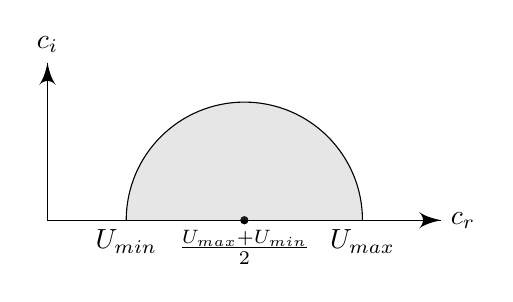
\begin{tikzpicture}
    \draw [->] (0, 0) -- (5, 0) node [right] {$c_r$};
    \draw [->] (0, 0) -- (0, 2) node [above] {$c_i$};

    \node [circ] at (2.5, 0) {};
    \node [below] at (2.5, 0) {$\frac{U_{max} + U_{min}}{2}$};
    \draw [fill=gray, fill opacity=0.2] (1, 0) arc (180:0:1.5);
    \node [below] at (1, 0) {$U_{min}$};
    \node [below] at (4, 0) {$U_{max}$};
  \end{tikzpicture}
\end{center}
Of course, lying within this region is a \emph{necessary} condition for instability to occur, but not \emph{sufficient}. The actual region of instability is a subset of this semi-circle, and this subset depends on the actual $\bar{U}$. But this is already very helpful, since if we way to search for instabilities, say numerically, then we know where to look.

\subsection{Stratified flows}
In the Kelvin--Helmholtz scenario, we had a varying density. Let's now try to model the situation in complete generality.

Recall that the set of (inviscid) equations for Boussinesq stratified fluids is
\[
  \rho \left(\frac{\partial \mathbf{u}}{\partial t} + \mathbf{u} \cdot \nabla \mathbf{u}\right) = - \nabla p' - g \rho' \hat{\mathbf{z}},
\]
with incompressibility equations
\[
  \nabla \cdot \mathbf{u} = 0,\quad \frac{\D \rho}{\D t} = 0.
\]
We consider a mean base flow and a $2D$ perturbation as a normal mode:
\begin{align*}
  \mathbf{u} &= \bar{U}(z) \hat{\mathbf{x}} + \mathbf{u}'(x, z, t)\\
  p &= \bar{p}(z) + p'(x, z, t)\\
  \rho &= \bar{\rho}(z) + \rho'(x, z, t),
\end{align*}
with
\[
  (\mathbf{u}', p', \rho') = [\hat{\mathbf{u}}(z), \hat{p}(z), \hat{\rho}(z)] e^{i(kx - \omega t)} = [\hat{\mathbf{u}}(z), \hat{p}(z), \hat{\rho}(z)] e^{ik(x - ct)}.
\]
We wish to obtain an equation that involves only $\hat{w}$. We first linearize our equations to obtain
\begin{align*}
  \bar{\rho} \left(\frac{\partial u'}{\partial t} + \bar{U} \frac{\partial u'}{\partial x} + w' \frac{\d \bar{U}}{\d z}\right) &= - \frac{\partial p'}{\partial x}\\
  \bar{\rho} \left(\frac{\partial w'}{\partial t} + \bar{U} \frac{\partial w'}{\partial x} \right) &= - \frac{\partial p'}{\partial z} - g \rho'\\
  \frac{\partial \rho'}{\partial t} + \bar{U} \frac{\partial \rho'}{\partial x} + w' \frac{\d \bar{\rho}}{\d z} &= 0\\
  \frac{\partial u'}{\partial x} + \frac{\partial w'}{\partial z} &= 0.
\end{align*}
Plugging in our normal mode solution into the four equations, we obtain
\begin{align*}
  ik \bar{\rho} (\bar{U} - c) \hat{u} + \bar{\rho} \hat{w} \frac{\d}{\d z} \bar{U} &= - ik\hat{p}\\
  ik \bar{\rho} (\bar{U} - c) \hat{w} &= - \frac{\d \hat{p}}{\d z} - g \hat{\rho}.\tag{$*$}\\
  ik(\bar{U} - c) \hat{\rho} + w' \frac{\d \bar{\rho}}{\d z} &= 0 \tag{$\dagger$}\\
  ik \hat{u} + \frac{\partial w'}{\partial z} &= 0.
\end{align*}
The last (incompressibility) equation helps us eliminate $\hat{u}$ from the first equation to obtain
\begin{align*}
  - \bar{\rho} (\bar{U} - c) \frac{\d \hat{w}}{\d z} + \bar{\rho} \hat{w} \frac{\d \bar{U}}{\d z} &= -ik \hat{p}.
\end{align*}
To eliminate $\hat{p}$ as well, we differentiate with respect to $z$ and apply $(*)$, and then further apply ($\dagger$) to get rid of the $\hat{\rho}$ term, and end up with
\[
  - \bar{\rho} (\bar{U} - c) \frac{\d^2 \hat{w}}{\d z^2} + \bar{\rho} \hat{w} \frac{\d^2 \bar{U}}{\d z^2} + k^2 \bar{\rho}(\bar{U} - c) \hat{w} = - \frac{g \hat{w}}{\bar{U} - c} \frac{\d \bar{\rho}}{\d z}.
\]
This allows us to write our equation as the \term{Taylor--Goldstein equation}
\[
  \left(\frac{\d^2}{\d z^2} - k^2\right) \hat{w} - \frac{\hat{w}}{(\bar{U} - c)} \frac{\d^2 \bar{U}}{\d z^2} + \frac{N^2 \hat{w}}{(\bar{U} - c)^2} = 0,
\]
where
\[
  N^2 = - \frac{g}{\bar{\rho}} \frac{\d \bar{\rho}}{\d z}.
\]
This $N$ is known as the \term{buoyancy frequency}, and has dimensions $T^{-2}$. This is the frequency at which a slab of stratified fluid would oscillate vertically.

Indeed, if we have a slab of volume $V$, and we displace it by an infinitesimal amount $\zeta$ in the vertical direction, then the buoyancy force is
\[
  F = Vg \zeta \frac{\partial \rho}{\partial z}.
\]
Since the mass of the fluid is $\rho_0 V$, by Newton's second law, the acceleration of the parcel satisfies
\[
  \frac{\d^2 \zeta}{\d t^2} + \left(- \frac{g}{\rho_0} \frac{\partial \rho}{\partial z}\right) \zeta = 0.
\]
This is just simple harmonic oscillation of frequency $N$.

Crucially, what we see from this computation is that a density stratification of the fluid can lead to \term{internal waves}. We will later see that the presence of these internal waves can destabilize our system.

\subsubsection*{Miles--Howard theorem}
In 1961, John Miles published a series of papers establishing a sufficient condition for infinitesimal stability in the case of a stratified fluid. When he submitted this to review, Louis Howard read the paper, and replied with a 3-page proof of a more general result. Howard's proof was published as a follow-up paper titled ``Note on a paper of John W.\ Miles''.

Recall that we just derived the Taylor--Goldstein equation
\[
  \left(\frac{\d^2}{\d z^2} - k^2\right) \hat{w} - \frac{\hat{w}}{(\bar{U} - c)} \frac{\d^2 \bar{U}}{\d z^2} + \frac{N^2 \hat{w}}{(\bar{U} - c)^2} = 0,
\]
The magical insight of Howard was to introduce the new variable
\[
  H = \frac{\hat{W}}{(\bar{U} - c)^{1/2}}.
\]
We can regretfully compute the derivatives
\begin{align*}
  \hat{w} &= (\bar{U} - c)^{1/2} H\\
  \frac{\d}{\d z} \hat{w} &= \frac{1}{2}(\bar{U} - c)^{-1/2} H \frac{\d \bar{U}}{\d z} + (\bar{U} - c)^{1/2} \frac{\d H}{\d z}\\
  \frac{\d^2}{\d z^2} \hat{w} &= - \frac{1}{4} (\bar{U} - c)^{-3/2} H \left(\frac{\d \bar{U}}{\d z}\right)^2 + \frac{1}{2} (\bar{U} - c)^{-1/2} H \frac{\d^2 \bar{U}}{\d z^2} \\
  &\hphantom{{}={}asdfadsf} + (\bar{U} - c)^{-1/2} \frac{\d H}{\d z} \frac{\d \bar{U}}{\d z} + (\bar{U} - c)^{1/2} \frac{\d^2 H}{\d z^2}.
\end{align*}

We can substitute this into the Taylor--Goldstein equation, and after some algebraic mess, we obtain the decent-looking equation
\[
  \frac{\d}{\d z}\left((\bar{U} - c) \frac{\d H}{\d z}\right) - H \left(k^2 (\bar{U} - c) + \frac{1}{2} \frac{\d^2 \bar{U}}{\d z^2} + \frac{\frac{1}{4} \left(\frac{\d \bar{U}}{\d z}\right)^2 - N^2}{\bar{U} - c}\right) = 0.
\]
This is now self-adjoint. Imposing boundary conditions $\hat{w}, \frac{\d \hat{w}}{\d z} \to 0$ in the far field, we multiply by $H^*$ and integrate over all space. The first term gives
\[
  \int H^* \frac{\d}{\d z} \left((\bar{U} - c)\frac{\d H}{\d z}\right)\;\d z = -\int (\bar{U} - c) \left|\frac{\d H}{\d z}\right|^2 \;\d z,
\]
while the second term is given by
\[
  \int \left(-k^2 |H|^2 (\bar{U} - c) - \frac{1}{2} \frac{\d^2\bar{U}}{\d z^2} |H|^2 - |H|^2 \frac{\left(\frac{1}{4} \left(\frac{\d \bar{U}}{\d z}\right)^2 - N^2\right) (\bar{U} - c^*)}{|\bar{U} - c|^2}\right)\;\d z.
\]
Both the real and imaginary parts of the sum of these two terms must be zero. In particular, the imaginary part reads
\[
  c_i \int \left(\abs{\frac{\d H}{\d z}}^2 + k^2 |H|^2 + |H|^2 \frac{N^2 - \frac{1}{4} \left(\frac{\d \bar{U}}{\d z}\right)^2}{|\bar{U} - c|^2}\right)\;\d z = 0.
\]
So a necessary condition for instability is that
\[
  N^2 - \frac{1}{4} \left(\frac{\d \bar{U}}{\d z}\right)^2 < 0
\]
somewhere. Defining the \term{Richardson number} to be
\[
  Ri(z) = \frac{N^2}{(\d \bar{U}/\d z)^2},
\]
the necessary condition is
\[
  Ri(z) < \frac{1}{4}.
\]
Equivalently, a \emph{sufficient} condition for stability is that $Ri(z) \geq \frac{1}{4}$ \emph{everywhere}.

How can we think about this? When we move a parcel, there is the buoyancy force that attempts to move it back to its original position. However, if we move the parcel to the high velocity region, we can gain kinetic energy from the mean flow. Thus, if the velocity gradient is sufficiently high, it becomes ``advantageous'' for parcels to move around.

\subsubsection*{Piecewise-linear profiles}
If we want to make our lives simpler, we can restrict our profile with piecewise linear velocity and layered density. In this case, to solve the Taylor--Goldstein equation, we observe that away from the interfaces, we have $N = U'' = 0$. So the Taylor--Goldstein equation reduces to
\[
  \left(\frac{\d^2}{\d z^2} - k^2\right) \hat{w} = 0.
\]
This has trivial exponential solutions in each of the individual regions, and to find the correct solutions, we need to impose some matching conditions at the interface.

So assume that the pressure is continuous across all interfaces. Then using the equation
\[
  - \bar{\rho} (\bar{U} - c) \frac{\d \hat{w}}{\d z} + \rho \hat{w} \frac{\d \bar{U}}{\d z} = -ik\hat{p},
\]
we see that the left hand seems like the derivative of a product, except the sign is wrong. So we divide by $\frac{1}{(\bar{U} - c)^2}$, and then we can write this as
\[
  \frac{ik}{\bar{\rho}} \frac{\hat{p}}{(\bar{U} - c)^2} = \frac{\d}{\d z}\left(\frac{\hat{w}}{\bar{U} - c}\right).
\]
For a general $c$, we integrate over an infinitesimal distance at the interface. We assume $\hat{p}$ is continuous, and that $\bar{\rho}$ and $(\bar{U} - c)$ have bounded discontinuity. Then the integral of the LHS vanishes in the limit, and so the integral of the right-hand side must be zero. This gives the matching condition
\[
  \left[ \frac{\hat{w}}{ \bar{U} - c}\right]^+_- = 0.
\]
To obtain a second matching condition, we rewrite the Taylor--Goldstein equation as a derivative, which allows for the determination of the other matching condition:
\[
  \frac{\d}{\d z} \left((\bar{U} - c) \frac{\d \hat{w}}{\d z} - \hat{w} \frac{\d \bar{U}}{\d z} - \frac{g \bar{\rho}}{\rho_0}\left(\frac{\hat{w}}{\bar{U} - c}\right)\right) = k^2 (\bar{U} - c)\hat{w} - \frac{g \bar{\rho}}{\rho_0} \frac{\d}{\d z} \left(\frac{\hat{w}}{\bar{U} - c}\right).
\]
Again integrating over an infinitesimal distance over at the interface, we see that the LHS must be continuous along the interface. So we obtain the second matching condition.
\[
  \left[(\bar{U} - c) \frac{\d \hat{w}}{\d z} - \hat{w} \frac{\d \bar{U}}{\d z} - \frac{g \bar{\rho}}{\rho_0}\left(\frac{\hat{w}}{\bar{U} - c}\right)\right]^+_- = 0.
\]
We begin by applying this to a relatively simple profile with constant density, and whose velocity profile looks like
\begin{center}
  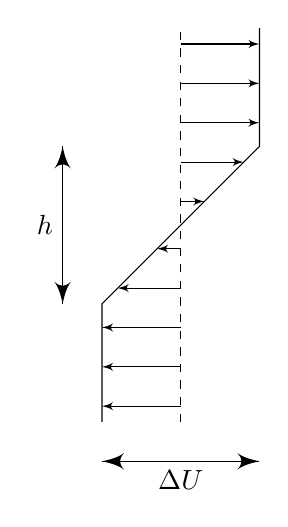
\begin{tikzpicture}
    \draw (-1, -2.5) -- (-1, -1) -- (1, 1) -- (1, 2.5);

    \draw [dashed] (0, -2.5) -- (0, 2.5);

    \foreach \y in {-1.3, -1.8, -2.3} {
      \draw [-latex'] (0, \y) -- (-1, \y);
      \draw [-latex'] (0, -\y) -- (1, -\y);
    }
    \foreach \x in {0.8, 0.3, -0.3, -0.8}{
      \draw [-latex'] (0, \x) -- (\x, \x);
    }

    \draw [<->] (-1.5, 1) -- (-1.5, -1) node [pos=0.5, left] {$h$};

    \draw [<->] (-1, -3) -- (1, -3) node [pos=0.5, below] {$\Delta U$};
  \end{tikzpicture}
\end{center}

For convenience, we scale distances by $\frac{h}{2}$ and speeds by $\frac{\Delta U}{2}$, and define $\tilde{c}$ and $\alpha$ by
\[
  c = \frac{\Delta U}{2} \tilde{c},\quad \alpha = \frac{kh}{2}.
\]
These quantities $\alpha$ and $\tilde{c}$ (which we will shortly start writing as $c$ instead) are nice dimensionless quantities to work with. After the scaling, the profile can be described by
\begin{center}
  \begin{tikzpicture}
    \draw [dashed] (-2, 1) -- (2, 1) node [right] {$z = 1$};
    \draw [dashed] (-2, -1) -- (2, -1) node [right] {$z = -1$};

    \draw (-1, -3) -- (-1, -1) node [pos=0.5, right] {$\bar{U} = -1$} -- (1, 1) node [pos=0.5, right] {$\bar{U} = z$} -- (1, 3) node [pos=0.5, right] {$\bar{U} =1$};
    \node at (-2, -2) {III};
    \node at (-2, 0) {II};
    \node at (-2, 2) {I};

    \node [right] at (3.5, 2) {$\hat{w} = Ae^{-\alpha(z - 1)}$};
    \node [right] at (3.5, 0) {$\hat{w} = Be^{\alpha z} + Ce^{-\alpha z}$};
    \node [right] at (3.5, -2) {$\hat{w} = D e^{\alpha (z + 1)}$};
  \end{tikzpicture}
\end{center}
We have also our exponential solutions in each region between the interfaces, noting that we require our solution to vanish at the far field.

We now apply the matching conditions. Since $\bar{U} - c$ is continuous, the first matching condition just says $\hat{w}$ has to be continuous. So we get
\begin{align*}
  A &= B e^\alpha + C e^{-\alpha}\\
  D &= B e^{-\alpha} + C e^{\alpha}.
\end{align*}
The other matching condition is slightly messier. It says
\[
  \left[(\bar{U} - c)\frac{\d \hat{w}}{\d z} - \hat{w} \frac{\d \bar{U}}{\d z} - \frac{g \bar{\rho}}{\rho_0} \left(\frac{\hat{w}}{\bar{U} - c}\right)\right]^+_- = 0,
\]
which gives us two equations
\begin{align*}
  (B e^\alpha + C e^{-\alpha}) (1 - c)(-\alpha) = (Be^\alpha - Ce^{-\alpha}) (1 - c)(\alpha) - (Be^\alpha + Ce^{-\alpha})\\
  (B e^{-\alpha} + C e^{\alpha}) (-1 - c)(\alpha) = (Be^{-\alpha} - Ce^{\alpha}) (-1 - c)(\alpha) - (Be^{-\alpha} + Ce^\alpha).
\end{align*}
Simplifying these gives us
\begin{align*}
  (2\alpha(1 - c) - 1) Be^\alpha &= Ce^{-\alpha}\\
  (2\alpha(1 + c) - 1) Ce^\alpha &= B e^{-\alpha}.
\end{align*}
Thus, we find that
\[
  (2\alpha - 1)^2 - 4\alpha^2 c^2 = e^{-4\alpha},
\]
and hence we have the dispersion relation
\[
  c^2 = \frac{(2\alpha - 1)^2 - e^{-4\alpha}}{4\alpha^2}.
\]
We see that this has the possibility of instability. Indeed, we can expand the numerator to get
\[
  c^2 = \frac{(1 - 4\alpha + 4\alpha^2) - (1 - 4\alpha + 8 \alpha^2 + O(\alpha^3))}{4\alpha^2} = -1 + O(\alpha).
\]
So for small $\alpha$, we have instability. This is known as \term{Rayleigh instability}. On the other hand, as $\alpha$ grows very large, this is stable. We can plot these out in a graph
\begin{center}
  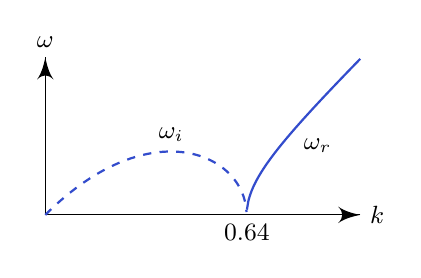
\begin{tikzpicture}[xscale=4, yscale=4]
    \draw [->] (0, 0) -- (1, 0) node [right] {\small$k$};
    \draw [->] (0, 0) -- (0, 0.5) node [above] {\small$\omega$};

    \draw [mblue, thick, dashed] plot coordinates {(0.000,0.00000) (0.005,0.00497) (0.010,0.00987) (0.015,0.01470) (0.020,0.01947) (0.025,0.02417) (0.030,0.02881) (0.035,0.03339) (0.040,0.03789) (0.045,0.04234) (0.050,0.04672) (0.055,0.05104) (0.060,0.05529) (0.065,0.05948) (0.070,0.06361) (0.075,0.06767) (0.080,0.07167) (0.085,0.07561) (0.090,0.07949) (0.095,0.08331) (0.100,0.08706) (0.105,0.09076) (0.110,0.09439) (0.115,0.09796) (0.120,0.10147) (0.125,0.10492) (0.130,0.10831) (0.135,0.11163) (0.140,0.11490) (0.145,0.11811) (0.150,0.12126) (0.155,0.12434) (0.160,0.12737) (0.165,0.13034) (0.170,0.13325) (0.175,0.13609) (0.180,0.13888) (0.185,0.14161) (0.190,0.14428) (0.195,0.14689) (0.200,0.14944) (0.205,0.15193) (0.210,0.15436) (0.215,0.15673) (0.220,0.15905) (0.225,0.16130) (0.230,0.16349) (0.235,0.16563) (0.240,0.16770) (0.245,0.16971) (0.250,0.17167) (0.255,0.17356) (0.260,0.17540) (0.265,0.17717) (0.270,0.17888) (0.275,0.18053) (0.280,0.18213) (0.285,0.18366) (0.290,0.18513) (0.295,0.18653) (0.300,0.18788) (0.305,0.18916) (0.310,0.19038) (0.315,0.19154) (0.320,0.19264) (0.325,0.19367) (0.330,0.19464) (0.335,0.19554) (0.340,0.19638) (0.345,0.19715) (0.350,0.19786) (0.355,0.19850) (0.360,0.19908) (0.365,0.19958) (0.370,0.20002) (0.375,0.20039) (0.380,0.20069) (0.385,0.20092) (0.390,0.20108) (0.395,0.20117) (0.400,0.20118) (0.405,0.20112) (0.410,0.20099) (0.415,0.20077) (0.420,0.20048) (0.425,0.20011) (0.430,0.19967) (0.435,0.19914) (0.440,0.19852) (0.445,0.19782) (0.450,0.19704) (0.455,0.19617) (0.460,0.19520) (0.465,0.19415) (0.470,0.19300) (0.475,0.19175) (0.480,0.19040) (0.485,0.18895) (0.490,0.18739) (0.495,0.18572) (0.500,0.18394) (0.505,0.18204) (0.510,0.18002) (0.515,0.17787) (0.520,0.17559) (0.525,0.17317) (0.530,0.17061) (0.535,0.16789) (0.540,0.16502) (0.545,0.16197) (0.550,0.15875) (0.555,0.15533) (0.560,0.15171) (0.565,0.14786) (0.570,0.14377) (0.575,0.13943) (0.580,0.13479) (0.585,0.12983) (0.590,0.12452) (0.595,0.11880) (0.600,0.11260) (0.605,0.10586) (0.610,0.09844) (0.615,0.09019) (0.620,0.08084) (0.625,0.06997) (0.630,0.05670) (0.635,0.03862) (0.639,0.00909)};
    \draw [mblue, thick] plot coordinates {(0.640,0.01655) (0.645,0.04562) (0.650,0.06270) (0.655,0.07632) (0.660,0.08809) (0.665,0.09868) (0.670,0.10844) (0.675,0.11757) (0.680,0.12622) (0.685,0.13447) (0.690,0.14240) (0.695,0.15005) (0.700,0.15747) (0.705,0.16469) (0.710,0.17174) (0.715,0.17863) (0.720,0.18538) (0.725,0.19201) (0.730,0.19854) (0.735,0.20496) (0.740,0.21129) (0.745,0.21755) (0.750,0.22373) (0.755,0.22984) (0.760,0.23588) (0.765,0.24187) (0.770,0.24781) (0.775,0.25370) (0.780,0.25954) (0.785,0.26534) (0.790,0.27110) (0.795,0.27682) (0.800,0.28251) (0.805,0.28816) (0.810,0.29378) (0.815,0.29938) (0.820,0.30495) (0.825,0.31049) (0.830,0.31601) (0.835,0.32151) (0.840,0.32698) (0.845,0.33244) (0.850,0.33787) (0.855,0.34329) (0.860,0.34869) (0.865,0.35407) (0.870,0.35944) (0.875,0.36480) (0.880,0.37014) (0.885,0.37546) (0.890,0.38078) (0.895,0.38608) (0.900,0.39137) (0.905,0.39665) (0.910,0.40192) (0.915,0.40718) (0.920,0.41242) (0.925,0.41767) (0.930,0.42290) (0.935,0.42812) (0.940,0.43333) (0.945,0.43854) (0.950,0.44374) (0.955,0.44894) (0.960,0.45412) (0.965,0.45930) (0.970,0.46448) (0.975,0.46964) (0.980,0.47480) (0.985,0.47996) (0.990,0.48511) (0.995,0.49026) (1.000,0.49540)};
     % map (\x -> (showFFloat (Just 3) x "", showFFloat (Just 5) ((sqrt $ -((2*x-1)^2-exp(-4*x))/4)) "")) ([0.000001] ++ [0.005,0.01..0.635] ++ [0.639])
     % map (\x -> (showFFloat (Just 3) x "", showFFloat (Just 5) ((sqrt $ ((2*x-1)^2-exp(-4*x))/4)) "")) ([0.64,0.645..1])

    \node [above] at (0.4, 0.20118) {\small$\omega_i$};
    \node [anchor = north west] at (0.79, 0.27110) {\small$\omega_r$};

    \node [below] at (0.64, 0) {\small$0.64$};
  \end{tikzpicture}
\end{center}

We see that the critical value of $\alpha$ is $0.64$, and the maximally instability point is $\alpha \approx 0.4$.

Let's try to understand where this picture came from. For large $k$, the wavelength of the oscillations is small, and so it seems reasonable that we can approximate the model by one where the two interfaces don't interact. So consider the case where we only have one interface.
\begin{center}
  \begin{tikzpicture}
    \draw [dashed] (-2, 1) -- (2, 1) node [right] {$z = 1$};

    \draw (-0.7, -0.7) -- (1, 1) node [pos=0.3, right] {$\bar{U} = z$} -- (1, 3) node [pos=0.5, right] {$\bar{U} =1$};

    \draw [dashed] (-0.7, -0.7) -- (-1.5, -1.5);

    \node at (-2, 0) {II};
    \node at (-2, 2) {I};

    \node [right] at (3.5, 2) {$Ae^{-\alpha(z - 1)}$};
    \node [right] at (3.5, 0) {$Be^{\alpha (z - 1)}$};
  \end{tikzpicture}
\end{center}
We can perform the same procedure as before, solving
\[
  \left[\frac{\hat{w}}{\bar{U} - c}\right]_-^+ = 0.
\]
This gives the condition $A = B$. The other condition then tell us
\[
  (1 - c) (-\alpha) A = (1 - c)\alpha A - Ae^{\alpha(z - 1)}.
\]
We can cancel the $A$, and rearrange this to say
\[
  c = 1 - \frac{1}{2\alpha}.
\]
So we see that this interface supports a wave at speed $c = 1 - \frac{1}{2\alpha}$ at a speed lower than $\bar{U}$. Similarly, if we treated the other interface at isolation, it would support a wave at $c_- = -1 + \frac{1}{2\alpha}$.

Crucially these two waves are individually stable, and when $k$ is large, so that the two interfaces are effectively in isolation, we simply expect two independent and stable waves. Indeed, in the dispersion relation above, we can drop the $e^{-4\alpha}$ term when $\alpha$ is large, and approximate
\[
  c = \pm \frac{2\alpha - 1}{2\alpha} = \pm \left(1 - \frac{1}{2\alpha}\right).
\]
When $k$ is small, then we expect the two modes to interact with each other, which manifests itself as the $-e^{4\alpha}$ term. Moreover, the resonance should be the greatest when the two modes have equal speed, i.e.\ at $\alpha \approx \frac{1}{2}$, which is quite close to actual maximally unstable mode.
%
%Physically, what is going on? The key aspect of the instability is that the exponential term $e^{-4\alpha}$ is negative. Where did this come from? If we look through our derivations, we see that these come from the interaction between the two interfaces.
%
%Indeed, suppose our fluid flow instead looks like
%\begin{center}
%  \begin{tikzpicture}
%    \draw [dashed] (-2, 0) -- (2, 0) node [right] {$z = 1$};
%
%    \draw (-2, -1) -- (1, 2) node [pos=0.5, right] {$\bar{U} = z$} -- (1, 4) node [pos=0.5, right] {$\bar{U} =1$};
%    \node at (-2, 1) {II};
%    \node at (-2, 3) {I};
%
%    %insert arrows?
%
%    \node at (2, -1) {$B e^{\alpha (z + 1)}$};
%    \node at (2, 3) {$Ae^{-\alpha(z - 1)}$};
%  \end{tikzpicture}
%\end{center}
%The first condition
%\[
%  \left[\frac{\hat{w}}{\bar{U} - c}\right]_-^+ = 0
%\]
%gives the condition $A = B$. The other condition then tell us
%\[
%  (1 - c) (-\alpha) A = (1 - c)\alpha A - Ae^{\alpha(z - 1)}.
%\]
%We can cancel the $A$, and rearrange this to say
%\[
%  c = 1 - \frac{1}{2\alpha}.
%\]
%So we see that this interface supports a wave at speed $c = 1 - \frac{1}{2\alpha}$ at a speed lower than $\bar{U}$. Similarly, if we treated the other interface at isolation, it would support a wave at $c_- = -1 + \frac{1}{2\alpha}$. % treating separately = large wavenumber.
%
%Now if $\alpha = \frac{1}{2}$, then $c_+ = c_- = 0$. Thus, the two speeds can resonate when $\alpha = \frac{1}{2}$, and this is when we expect to have the worst instability.
%
%We can also see this by writing our dispersion relation by
%\[
%  c^2 = \left(1 - \frac{1}{2\alpha}\right)^2 - \frac{e^{-4\alpha}}{4\alpha^2}.
%\]
%We see that if we ignore the second term, then this is the same as saying that the possible speeds are $\pm \left(1 - \frac{1}{3\alpha}\right)$. The second term gives us the interaction between the two interfaces, and we see that this interaction is what gives rise to the instability.

\subsubsection*{Density stratification}
We next consider the case where we have \term{density stratification}. After scaling, we can draw our region and solutions as
\begin{center}
  \begin{tikzpicture}
    \draw [dashed] (-2, 0) -- (2, 0) node [right] {$z = -1$};
    \draw [dashed] (-2, 1) -- (2, 1) node [right] {$z = 0$};

    \draw [dashed] (-2, 2) -- (2, 2) node [right] {$z = 1$};
    \draw (-1, -2) -- (-1, 0) node [pos=0.5, right] {$\bar{U} = -1$} -- (1, 2) node [pos=0.7, right] {$\bar{U} = z$} -- (1, 4) node [pos=0.5, right] {$\bar{U} =1$};
    \node at (-2, 0.5) {III};
    \node at (-2, -1) {IV};
    \node at (-2, 1.5) {II};
    \node at (-2, 3) {I};

    \node [right] at (3.5, 3) {$Ae^{-\alpha(z - 1)}$};
    \node [right] at (3.5, 1.5) {$Be^{\alpha(z - 1)} + C e^{-\alpha(z - 1)}$};
    \node [right] at (3.5, 0.5) {$De^{\alpha (z + 1)} + E e^{-\alpha(z + 1)}$};
    \node [right] at (3.5, -1) {$F e^{\alpha (z + 1)}$};

    \draw [mred] (-1, 4) node [above] {$\bar{\rho} = -1$} -- (-1, 1) -- (1, 1) -- (1, -2) node [below] {$\bar\rho = +1$};
  \end{tikzpicture}
\end{center}
Note that the $\bar{\rho}$ is the relative density, since it is the density difference that matters (fluids cannot have negative density).

Let's first try to understand how this would behave heuristically. As before, at the I-II and III-IV interfaces, we have waves with $c = \pm \left(1 - \frac{1}{2\alpha}\right)$. At the density interface, we previously saw that we can have \term{internal gravity waves} with $c_{igw} = \pm \sqrt{\frac{Ri_0}{\alpha}}$, where
\[
  Ri_0 = \frac{g h}{\rho_0}
\]
is the \term{bulk Richardson number} (before scaling, it is $Ri_0 = \frac{g \Delta \rho h}{\rho_0 \Delta U^2}$).

We expect instability to occur when the frequency of this internal gravity wave aligns with the frequency of the waves at the velocity interfaces, and this is given by
\[
  \left(1 - \frac{1}{2\alpha}\right)^2 = \frac{Ri_0}{\alpha}.
\]
It is easy to solve this to get the condition
\[
  Ri_0 \simeq \alpha - 1.
\]
This is in fact what we find if we solve it exactly.

So let's try to understand the situation more responsibly now. The procedure is roughly the same. The requirement that $\hat{w}$ is continuous gives
\begin{align*}
  A &= B + C\\
  B e^{-\alpha} + C e^\alpha &= D e^\alpha + E e^{-\alpha}\\
  D + E &= F.
\end{align*}
If we work things out, then the other matching condition
\[
  \left[(\bar{U} - c) \frac{\d \hat{w}}{\d z} - \hat{w} \frac{\d \bar{U}}{\d z} - Ri_0 \bar{\rho} \left(\frac{\hat{w}}{\bar{U} - c}\right)\right]^+_- = 0
\]
gives
\begin{align*}
  (1 - c)(-\alpha) A &= (1 - c)(\alpha) (B - C) - (B + C)\\
  (-1 - c)(\alpha) F &= (-1 - c)(\alpha) (D - E) - (D + E)
\end{align*}
\begin{multline*}
  (-c)(\alpha) (B e^{-\alpha} - C e^\alpha) + \frac{Ri_0}{(-c)} (Be^{-\alpha} + C e^\alpha) \\
  = (-c)(\alpha) (De^\alpha - E e^{-\alpha}) - \frac{Ri_0}{(-c)} (De^\alpha + Ee^{-\alpha}).
\end{multline*}
%
%
%What happens when we have stratification? In that case, we have interfacial gravity waves too, with
%\[
%  \omega^2 = \frac{g(\rho_1 - \rho_2) k}{\rho_1 + \rho_2}.
%\]
%These have % star on dimensional quantities % u^* = \Delta u^*/2 u,\quad c^* = \Delta u^*/2 c,\quad z^* = d^*/2 z,\quad \bar{\rho}^* = \Delta \rho^2/2 \bar{\rho}. So \bar{\rho} = \frac{2 \rho_0^*}{\Delta \rho^*} \mp 1
%\[
%  c_{igw \pm} = \left(\frac{Ri_0}{\alpha}\right)^{1/2}.
%\]
%How does their presence modify stability? Recall we were scaling lengths by $\frac{h^*}{2}$, and
%\[
%  J = Ri_0 = \frac{g^* \Delta \rho^* h^*}{\rho_0^* (\Delta U^*)^2}.
%\]
%Then the natural thing to say is that
%\[
%  \rho_1^* = \rho^* + \frac{\Delta \rho^*}{2},\quad \rho_2^* = \rho_0^* - \frac{\Delta \rho^*}{2}.
%\]
%Then we have
%\[
%  (\omega^*)^2 = c^{*2} h^{*2} = \frac{g^* \Delta \rho^* k^*}{2 \rho_0^*}.
%\]
%To non-dimensionalize this, we as usual put
%\[
%  c^* = \frac{\Delta U}{2} c,\quad k^* = \frac{2h}{\alpha}.
%\]
%We then get
%\[
%  \frac{(\Delta u^*)^2}{4} \frac{4}{h^{*2}} \alpha^2 c^2 = \frac{g^* \Delta \rho^*}{2 \rho_0^*} \frac{2}{h} \alpha.
%\]
%Cancelling terms, we are left with
%\[
%  c^2 = \left(\frac{g^* \Delta \rho^* h^*}{\rho_0^*(\Delta u^*)^2}\right)/\alpha = \frac{Ri_0}{\alpha}.
%\]
%
%We now have three interfaces. The condition $\left[\frac{\hat{w}}{\bar{U} - c}\right]^+_- = 0$ is simple. We get the conditions
%\begin{align*}
%  A &= B + C\\
%  B e^{-\alpha} + C e^\alpha &= D e^\alpha + E e^{-\alpha}\\
%  D + E &= F.
%\end{align*}
%If we work things out, then the other (non-dimensionalized) matching condition
%\[
%  \left[(\bar{U} - c) \frac{\d \hat{w}}{\d z} - \hat{w} \frac{\d \bar{U}}{\d z} - Ri_0 \bar{\rho} \left(\frac{\hat{w}}{\bar{U} - c}\right)\right]^+_- = 0
%\]
%gives
%\begin{align*}
%  (1 - c)(-\alpha) A &= (1 - c)(\alpha) (B - C) - (B + C)\\
%  (-1 - c)(\alpha) F &= (-1 - c)(\alpha) (D - E) - (D + E)\\
%  &(-c)(\alpha) (B e^{-\alpha} - C e^\alpha) + \frac{Ri_0}{(-c)} (Be^{-\alpha} + C e^\alpha) \\
%  &= (-c)(\alpha) (De^\alpha - E e^{-\alpha}) - \frac{Ri_0}{(-c)} (De^\alpha + Ee^{-\alpha}).
%\end{align*}
This defines a $6 \times 6$ matrix problem, 4th order in $c$. Writing it as $S\mathbf{X} = 0$ with $\mathbf{X} = (A, B, C, D, E, F)^T$, the existence of non-trivial solutions is given by the requirement that $\det S = 0$, which one can check (!) is given by
\[
  c^4 + c^2 \left(\frac{e^{-4\alpha} - (2\alpha - 1)^2}{4\alpha^2} - \frac{Ri_0}{\alpha}\right) + \frac{Ri_0}{\alpha} \left(\frac{e^{-2\alpha} + (2\alpha - 1)}{2\alpha}\right)^2 = 0.
\]
This is a biquadratic equation, which we can solve.

We can inspect the case when $Ri_0$ is very small. In this case, the dispersion relation becomes
\[
  c^4 + c^2 \left(\frac{e^{-4\alpha} - (2\alpha - 1)^2}{4\alpha^2}\right).
\]
Two of these solutions are simply given by $c = 0$, and the other two are just those we saw from Rayleigh instability. This is saying that when the density difference is very small, then the internal gravitational waves are roughly non-existent, and we can happily ignore them.

In general, we have instability for all $Ri_0$! This is \term{Holmboe instability}. The scenario is particularly complicated if we look at small $\alpha$, where we expect the effects of Rayleigh instability to kick in as well. So let's fix some $0 < \alpha < 0.64$, and see what happens when we increase the Richardson number. % insert full contour picture

As before, we use dashed lines to denote the imaginary parts and solid lines to denote the real part. For each $Ri_0$, any combination of imaginary part and real part gives a solution for $c$, and, except when there are double roots, there should be four such possible combinations.
\newcommand{\AAA}{0.25296}
\newcommand{\DDD}{1.57055}
\begin{center}
  \begin{tikzpicture}[xscale=100, yscale=2.8]
    \pgfmathdeclarefunction{imsqrt}{2}{\pgfmathparse{((#1)^2 + (#2)^2)^(1/4) * sin (90 + 1/2 * atan (#2 / #1))}}
    \pgfmathdeclarefunction{resqrt}{2}{\pgfmathparse{((#1)^2 + (#2)^2)^(1/4) * cos (90 + 1/2 * atan (#2 / #1))}}

    \draw [->] (0, 0) -- (0.05, 0) node [right] {$Ri_0$}; % = Ri?
    \draw [->] (0, -1) -- (0, 1) node [above] {$c$};

    \draw [semithick, domain=0:0.0205, samples=50, dashed, mblue] plot (\x, {sqrt(-(\x - \AAA - sqrt(\x^2 - 2 * \DDD * \x + (\AAA)^2)))});
    \draw [semithick, domain=0:0.0205, samples=50, dashed, mblue] plot (\x, {sqrt(-(\x - \AAA + sqrt(\x^2 - 2 * \DDD * \x + (\AAA)^2)))});

    \draw [semithick, domain=0.0206:0.049, samples=50, dashed, mblue] plot (\x, {imsqrt(\x - \AAA, sqrt(-(\x^2 - 2 * \DDD * \x + (\AAA)^2)))});

    \draw [semithick, mblue] (0, 0) -- (0.0205, 0);
    \draw [semithick, domain=0.020506:0.049, samples=50, mblue] plot (\x, {resqrt(\x - \AAA, sqrt(-(\x^2 - 2 * \DDD * \x + (\AAA)^2)))});

    \draw [semithick, domain=0:0.0205, samples=50, dashed, mblue] plot (\x, {-sqrt(-(\x - \AAA - sqrt(\x^2 - 2 * \DDD * \x + (\AAA)^2)))});
    \draw [semithick, domain=0:0.0205, samples=50, dashed, mblue] plot (\x, {-sqrt(-(\x - \AAA + sqrt(\x^2 - 2 * \DDD * \x + (\AAA)^2)))});

    \draw [semithick, domain=0.0206:0.049, samples=50, dashed, mblue] plot (\x, {-imsqrt(\x - \AAA, sqrt(-(\x^2 - 2 * \DDD * \x + (\AAA)^2)))});

    \draw [semithick, domain=0.020506:0.049, samples=50, mblue] plot (\x, {-resqrt(\x - \AAA, sqrt(-(\x^2 - 2 * \DDD * \x + (\AAA)^2)))});
  \end{tikzpicture}
\end{center}
We can undersatnd this as follows. When $Ri_0 = 0$, all we have is Rayleigh instability, which are the top and bottom curves. There are then two $c = 0$ solutions, as we have seen. As we increase $Ri_0$ to a small, non-sero amount, this mode becomes non-zero, and turns into a genuine unstable mode. As the value of $Ri_0$ increases, the two imaginary curves meet and merge to form a new curve. The solutions then start to have a non-zero real part, which gives a non-zero phase speed to our pertrubation.

Note that when $Ri_0$ becomes very large, then our modes become unstable again, though this is not clear from our graph.

%
%
%In general, the phase speed of the perturbation is non-zero, and actually the instability lies between the interfaces.
%
%Note that this does not violate Miles--Howard, since $Ri = 0$ on either side of the density of the interface.
%
%Let's fix some $0 < \alpha < 0.64$, so that we have Rayleigh instability. Note that if $c$ is a complex root, then we know the roots are just $\{\pm c, \pm \bar{c}\}$. Plotting $c_r$ and $c_i$ separately,
%
%\begin{center}
%  \begin{tikzpicture}
%    \draw [->] (-1, 0) -- (5, 0) node [right] {$J$}; % = Ri?
%    \draw (0, -3) -- (0, 3);
%    \draw [morange, thick] (0, 2) edge [bend left] (2, 0.8);
%    \draw [morange, thick] (0, 0) edge [bend right] (2, 0.8) edge [bend left] (4, 0);
%
%    \draw [mred, thick] (0, 0) -- (2, 0) edge [bend left] (4, 0.6); % reflect all these
%  \end{tikzpicture}
%\end{center}
%The orange lines are the imaginary parts, and the red lines are the real parts. When $J = 0$, we have Rayleigh instability, so we have one unstable mode, one decaying mode and two zero modes. As we increase $J$, the zero modes increase in imaginary parts, but the phase speed remains constant.
%
%When the two curves meet, they combine to give Holmboe instability, and the phase speed starts to increase.
\subsubsection*{Taylor instability}
While Holmboe instability is quite interesting, our system was unstable even without the density stratification. Since we saw that instability is in general triggered by the interaction between two interfaces, it should not be surprising that even in a Rayleigh stable scenario, if we have two layers of density stratification, then we can still get instability.

Consider the following flow profile:
\begin{center}
  \begin{tikzpicture}
    \draw [dashed] (-2, 1) -- (2, 1) node [right] {$z = 1$};
    \draw [dashed] (-2, -1) -- (2, -1) node [right] {$z = -1$};

    \draw (-1, -3) -- (1, 3) node [pos=0.5, right] {$\bar{U} =z$};

    \foreach \y in {0.75, 1.25, 1.75, 2.25, 2.75} {
      \draw [-latex'] (0, \y) -- (\y/3, \y);
      \draw [-latex'] (0, -\y) -- (-\y/3, -\y);
    }
    \draw [dashed] (0, -3) -- (0, 3);

    \node at (-2, -2) {III};
    \node at (-2, 0) {II};
    \node at (-2, 2) {I};

    \node [right] at (3.5, 2) {$Ae^{-\alpha(z - 1)}$};
    \node [right] at (3.5, 0) {$Be^{\alpha z} + Ce^{-\alpha z}$};
    \node [right] at (3.5, -2) {$D e^{\alpha (z + 1)}$};

    \draw [mred] (-0.7, 3) node [above] {\small$\bar{\rho} = R - 1$} -- (-0.7, 1) -- (0, 1) -- (0, -1) --(0.7, -1) -- (0.7, -3) node [below] {\small$\bar{\rho} = R + 1$};
  \end{tikzpicture}
\end{center}
As before, continuity in $\hat{w}$ requires
\begin{align*}
  A &= Be^\alpha + Ce^{-\alpha}\\
  D &= Be^{-\alpha} + Ce^{\alpha}.
\end{align*}
Now there is no discontinuity in vorticity, but the density field has jumps. So we need to solve the second matching condition. They are
\begin{align*}
  (1 - c) (-\alpha) (Be^\alpha + C e^{-\alpha}) + \frac{Ri_0}{1 - c} (B e^\alpha + Ce^{-\alpha}) &= (1 - c)(\alpha) (Be^\alpha - C e^{-\alpha})\\
  (1 - c)(\alpha) (Be^{-\alpha} + Ce^\alpha) + \frac{Ri_0}{1 + c} (B e^{-\alpha} + C e^\alpha) &= (-1 - c)(\alpha)(Be^\alpha - Ce^\alpha)
\end{align*}
These give us, respectively,
\begin{align*}
  (2\alpha(1 - c)^2 - Ri_0)B &= Ri_0 Ce^{-2\alpha}\\
  (2\alpha(1 + c)^2 - Ri_0)C &= Ri_0 Be^{-2\alpha}.
\end{align*}
So we get the biquadratic equation
\[
  c^4 - c^2 \left(2 + \frac{Ri_0}{\alpha}\right) + \left(1 - \frac{Ri_0}{2\alpha}\right)^2 - \frac{Ri_0^2 e^{-4\alpha}}{4\alpha^2} = 0.
\]
We then apply the quadratic formula to say
\[
  c^2 = 1 + \frac{Ri_0}{2\alpha} \pm \sqrt{\frac{2Ri_0}{\alpha} + \frac{Ri_0^2 e^{-4\alpha}}{4\alpha^2}}.
\]
So it is possible to have instability with no inflection! Indeed, instability occurs when $c^2 < 0$, which is equivalent to requiring
\[
  \frac{2\alpha}{1 + e^{-2\alpha}} < Ri_0 < \frac{2\alpha}{1 - e^{-2\alpha}}.
\]
Thus, for any $Ri_0 > 0$, we can have instability. This is known as \term{Taylor instability}.

Heuristically, the density jumps at the interface have speed
\[
  c_{igw}^{\pm} = \pm 1 \mp \left(\frac{Ri_0}{2\alpha}\right)^{1/2}.
\]
We get equality when $c = 0$, so that $Ri_0 = 2\alpha$. This is in very good agreement with what our above analysis gives us.

% insert contour picture


\section{Absolute and convective instabilities}

So far, we have only been considering perturbations that are Fourier modes,
\[
  (\mathbf{u}', p', \rho') = [\hat{\mathbf{u}}(z), \hat{p}(z), \hat{\rho}(z)]e^{i(\mathbf{k}\cdot \mathbf{x} - \omega t}.
\]
This gives rise to a dispersion relation $D(\mathbf{k}, \omega) = 0$. This is an eigenvalue problem for $\omega(\mathbf{k})$, and the $k$th mode is unstable if the solution $\omega(k)$ has positive imaginary part.

When we focus on Fourier modes, they are necessarily non-local. In reality, perturbations tend to be local. We perturb the fluid at some point, and the perturbation spreads out. In this case, we might be interested in \emph{how} the perturbations spread.

To understand this, we need the notion of \term{group velocity}. For simplicity, suppose we have a sum of two Fourier modes of slightly different wavenumbers $k_0 \pm k_\Delta$. The corresponding frequencies are then $\omega_0 \pm \omega_\Delta$, and for small $k_\Delta$, we may approximate
\[
  \omega_\Delta = k_\Delta \left.\frac{\partial \omega}{\partial k}\right|_{k = k_0}.
\]
We can then look at how our wave propagates:
\begin{align*}
  \eta &= \cos [(k_0 + k_\Delta)x - (\omega_0 + \omega_\Delta)t] + \cos [k_0 - k_\Delta)x - (\omega_0 - \omega_\Delta)t]\\
  &= 2 \cos (k_\Delta x - \omega_\Delta t) \cos (k_0 x - \omega_0 t)\\
  &= 2 \cos \left(k_\Delta \left(w - \left.\frac{\partial \omega}{\partial k}\right|_{k = k_0}t\right)\right) \cos (k_0 x - \omega_0 t)
\end{align*}
Since $k_\Delta$ is small, we know the first term has a long wavelength, and determines the ``overall shape'' of the wave.

\begin{center}
  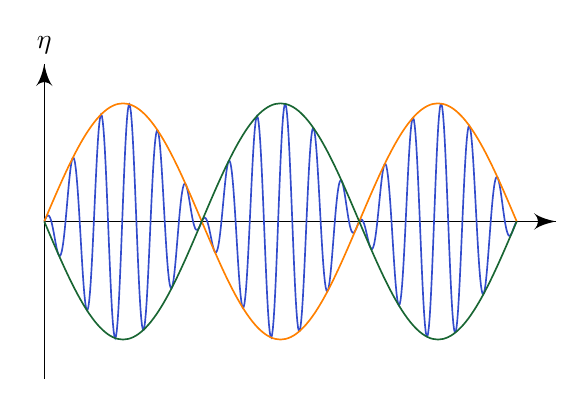
\begin{tikzpicture}
    \draw [->] (0, 0) -- (6.5, 0);
    \draw [->] (0, -2) -- (0, 2) node [above] {$\eta$};

    \draw [semithick, mblue, domain=0:6,samples=600] plot(\x, {1.5 * cos(1000 * \x) * sin (90 * \x)});
    \draw [semithick, morange] (0, 0) sin (1, 1.5) cos (2, 0) sin (3, -1.5) cos (4, 0) sin (5, 1.5) cos (6, 0);
    \draw [semithick, mgreen] (0, 0) sin (1, -1.5) cos (2, 0) sin (3, 1.5) cos (4, 0) sin (5, -1.5) cos (6, 0);
  \end{tikzpicture}
\end{center}

As time evolves, these ``packets'' propagate with \term{group velocity} $c_g = \frac{\partial \omega}{\partial k}$. This is also the speed at which the energy in the wave packets propagate.

In general, there are 4 key characteristics of interest for these waves:
\begin{itemize}
  \item The energy in a wave packet propagates at a \term{group velocity}.
  \item They can \emph{disperse} (different wavelengths have different speeds)
  \item They can be \emph{advected} by a streamwise flow.
  \item They can be \emph{unstable}, i.e.\ their amplitude can grow in time and space.
\end{itemize}

In general, if we have an unstable system, then we expect the perturbation to grow with time, but also ``move away'' from the original source of perturbation. We can consider two possibilities --- we can have \term{convective instability}, where the perturbation ``goes away''; and \term{absolute instability}, where the perturbation doesn't go away.

We can imagine the evolution of a convective instability as looking like this:
\begin{center}
  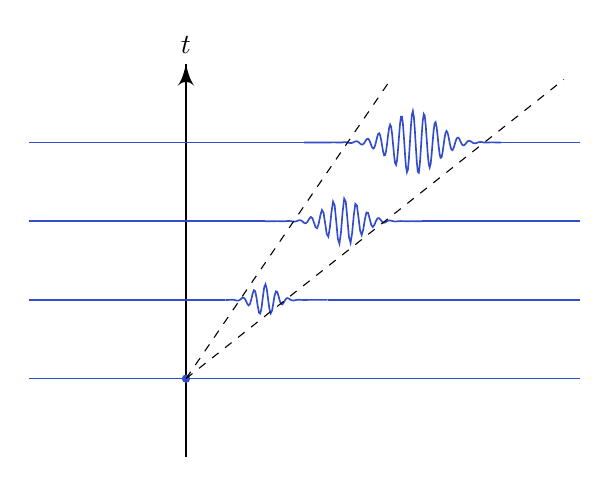
\begin{tikzpicture}
    \draw [->] (0, -1) -- (0, 4) node [above] {$t$};

    \draw [semithick, mblue] (-2, 0) -- (5, 0);

    \draw [semithick, mblue] (-2, 1) -- (0.5, 1);
    \draw [semithick, mblue] (-2, 2) -- (1, 2);
    \draw [semithick, mblue] (-2, 3) -- (1.5, 3);

    \draw [semithick, mblue] (1.8, 1) -- (5, 1);
    \draw [semithick, mblue] (3, 2) -- (5, 2);
    \draw [semithick, mblue] (4, 3) -- (5, 3);

    \node [circ, mblue] at (0, 0) {};
    \draw [semithick, mblue, domain=0.5:1.8,samples=80] plot (\x, {1 + 0.2 * cos(2500 * \x) * exp (- 25 * ((\x - 1)^2))});
    \draw [semithick, mblue, domain=1:3,samples=100] plot (\x, {2 + 0.3 * cos(2500 * \x) * exp (- 10 * ((\x - 2)^2))});
    \draw [semithick, mblue, domain=1.5:4,samples=200] plot (\x, {3 + 0.4 * cos(2500 * \x) * exp (- 6 * ((\x - 2.9)^2))});

    \draw [dashed] (0, 0) -- (2.6, 3.8);
    \draw [dashed] (0, 0) -- (4.8, 3.8);
  \end{tikzpicture}
\end{center}
whereas an absolute instability would look like this:
\begin{center}
  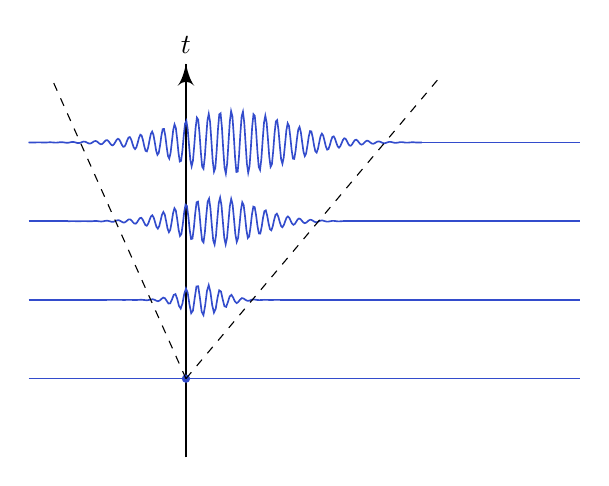
\begin{tikzpicture}
    \draw [->] (0, -1) -- (0, 4) node [above] {$t$};

    \draw [semithick, mblue] (-2, 0) -- (5, 0);

    \draw [semithick, mblue] (-2, 1) -- (-1, 1);
    \draw [semithick, mblue] (-2, 2) -- (-1.5, 2);
    \draw [semithick, mblue] (-2, 3) -- (-2, 3);

    \draw [semithick, mblue] (1.2, 1) -- (5, 1);
    \draw [semithick, mblue] (2, 2) -- (5, 2);
    \draw [semithick, mblue] (3, 3) -- (5, 3);
    \node [circ, mblue] at (0, 0) {};

    \draw [semithick, mblue, domain=-1:1.2,samples=100] plot (\x, {1 + 0.2 * cos(2500 * \x) * exp (- 8 * ((\x - 0.2)^2))});
    \draw [semithick, mblue, domain=-1.5:2,samples=200] plot (\x, {2 + 0.3 * cos(2500 * \x) * exp (- 2 * ((\x - 0.4)^2))});
    \draw [semithick, mblue, domain=-2:3,samples=300] plot (\x, {3 + 0.4 * cos(2500 * \x) * exp (- ((\x - 0.6)^2))});

    \draw [dashed] (0, 0) -- (-1.7, 3.8);
    \draw [dashed] (0, 0) -- (3.2, 3.8);
  \end{tikzpicture}
\end{center}

Note that even in the absolute case, the perturbation may still have non-zero group velocity. It's just that the perturbations grow more quickly than the group velocity.

To make this more precise, we consider the response of the system to an \emph{impulse}. We can understand the dispersion relation as saying that in phase space, a quantity $\chi$ (e.g.\ velocity, pressure, density) must satisfy
\[
  D(k, \omega) \tilde{\chi}(k, \omega) = 0,
\]
where
\[
  \tilde{\chi}(k, \omega) = \int_{-\infty}^\infty\int_{-\infty}^\infty \chi(x, t) e^{-i(kx - \omega t)}\;\d x\;\d t.
\]
Indeed, this equation says we can have a non-zero $(k, \omega)$ mode iff they satisfy $D(k, \omega) = 0$. The point of writing it this way is that this is now linear in $\tilde{\chi}$, and so it applies to any $\chi$, not necessarily a Fourier mode.

Going back to position space, we can think of this as saying
\[
  \D \left(-i \frac{\partial}{\partial x}, i\frac{\partial}{\partial t}\right) \chi(x, t) = 0.
\]
This equation allows us to understand how the system responds to some external forcing $F(x, t)$. We simply replace the above equation by
\[
  \D \left(-i\frac{\partial}{\partial x}, i\frac{\partial}{\partial t}\right) \chi(x, t) = F(x,t).
\]
Usually, we want to solve this in Fourier space, so that
\[
  D(k, \omega) \tilde{\chi}(k, \omega) = \tilde{F}(k, \omega).
\]
In particular, the \term{Green's function} (or \term{impulse response}) is given by the response to the impulse $F_{\xi, \tau}(x, t) = \delta(x - \xi) \delta(t - \tau)$. We may wlog assume $\xi = \tau = 0$, and just call this $F$. The solution is, by definition, the \term{Green's function} $G(x, t)$, satisfying
\[
  \D \left(-i\frac{\partial}{\partial x}, i\frac{\partial}{\partial t}\right) G(x, t) = \delta(x)\delta(t).
\]
Given the Green's function, the response to an arbitrary forcing $F$ is ``just'' given by
\[
  \chi(x, t) = \int G(x - \xi, t - \tau) F(\xi, \tau)\;\d \xi \;\d \tau.
\]
Thus, the Green's function essentially controls the all behaviour of the system.

%Once there is the possibility of spatial instability, it is essential to consider response to perturbations. This gives a different (but equivalent) definitions of linear instability in terms of impulse response.
%
%Consider we are in (for simplicity) 2D and we have a dispersion relation $D(k, \omega; R) = 0$. Then the eigenfunction (dependent on $z$) is completely determined from $D$. We are interested in the response of some complex scalar field $\chi(x, t)$ to some forcing.
%
%The dispersion relation effectively defines a linear partial differential operator on $\chi(x, t)$:
%Indeed, if $F = 0$ and $\chi(x, t) = Ae^{i(kx - \omega t)}$, then this simply says $D(k, \omega; R) = 0$.
%
%Then the central problem reduces to the determination of Green's function of this operator:
%\[
%  \D \left(-i\frac{\partial}{\partial x}, i \frac{\partial}{\partial t}; R\right) G(x, t; \xi, \tau) = \delta(x - \xi) \delta(t - \tau).
%\]
%Then the solution to our PDE above is just
%\[
%  \chi(x, t) = \int G(x, t; \xi, \tau) F(\xi, \tau)\;\d \xi\;\d \tau.
%\]
%of course, we may perform a shift to make the impulse at $x = 0, t = 0$. So $G$ is the \term{impulse response}.

With the Green's function, we may now make some definitions.
\begin{defi}[Linear stability]\index{linear stability}
  The base flow of a system is \emph{linearly stable} if
  \[
    \lim_{t \to \infty} G(x, t) = 0
  \]
  along \emph{all} rays $\frac{x}{t} = C$.

  A flow is unstable if it is not stable.
\end{defi}

\begin{defi}[Linearly convectively unstable]\index{linear convective instability}\index{convective instability!linear}
  An unstable flow is \emph{linearly convectively unstable} if $\lim_{t \to \infty}G(x, t) = 0$ along the ray $\frac{x}{t} = 0$.
\end{defi}
\begin{defi}[Linearly absolutely unstable]\index{linear absolute instability}\index{absolute instability!linear}
  An unstable flow is \term{linearly absolutely unstable} if $\lim_{t\to \infty}G(x, t) \not= 0$ along the ray $\frac{x}{t} = 0$.
\end{defi}

The first case is what is known as an \term{amplifier}, where the instability grows but travels away at the same time. In the second case, we have an \term{oscillator}.

Even for a general $F$, it is easy to solve for $\tilde{\chi}$ in Fourier space. Indeed, we simply have
\[
  \tilde{\chi}(k, \omega) = \frac{\tilde{F}(k, \omega)}{D(k, \omega)}.
\]
To recover $\chi$ from this, we use the Fourier inversion formula
\[
  \chi(x, t) = \frac{1}{(2\pi)^2} \int_{L_\omega} \int_{F_k} \tilde{\chi}(k, \omega) e^{i(kx - \omega t)}\;\d k\;\d \omega.
\]
Note that here we put some general contours for $\omega$ and $k$ instead of integrating along the real axis, so this is not the genuine Fourier inversion formula. However, we notice that as we deform our contour, when we pass through a singularity, we pick up a multiple of $e^{i(kx - \omega t)}$. Moreover, since the singularities occur when $D(k, \omega) = 0$, it follows that these extra terms we pick up are in fact solutions to the homogeneous equation $D(-i\partial_x, i\partial_t) \chi = 0$. Thus, no matter which contour we pick, we do get a genuine solution to our problem.

So how should we pick a contour? The key concept is \emph{causality} --- the response must come after the impulse. Thus, if $F(x, t) = 0$ for $t < 0$, then we also need $\chi(x, t) = 0$ in that region. To understand this, we perform only the temporal part of the Fourier inversion, so that
\[
  \tilde{\chi}(k, t) = \frac{1}{2\pi}\int_{L_\omega} \frac{\tilde{F}(k, \omega)}{D(k, \omega; R)} e^{-i\omega t}\;\d \omega.
\]
To perform this contour integral, we close our contour either upwards or downwards, compute residues, and then take the limit as our semi-circle tends to infinity. For this to work, it must be the case that the contribution by the circular part of the contour vanishes in the limit, and this determines whether we should close upwards or downwards.

If we close upwards, then $\omega$ will have positive imaginary part. So for $e^{-i\omega t}$ not to blow up, we need $t < 0$. Similarly, we close downwards when $t > 0$. Thus, if we want $\chi$ to vanish whenever $t < 0$, we should pick our contour so that it it lies above all the singularities, so that it picks up no residue when we close upwards. This determines the choice of contour.

But the key question is which of these are causal. When $t < 0$, we require $\chi(k, t) < 0$. By Jordan's lemma, for $t < 0$, when performing the $\omega$ integral, we should close the contour upwards when when perform the integral; when $t > 0$, we close it downwards. Thus for $\chi(k, t) = 0$ when $t < 0$, we must pick $L_\omega$ to lie \emph{above} all singularities of $\tilde{\chi}(k, \omega)$.

%Now recall our Fourier transformed problem
%\[
%  \tilde{D}(k, \omega; R) \tilde{\chi}(k, \omega) = \tilde{F}(k, \omega).
%\]
%In the absence of forcing, i.e.\ $F = 0$, we recover the normal modes with $\tilde{D}(k, \omega; R) = 0$.
%
%With forcing, we can formally construct
%\[
%  \tilde{\chi}(k, \omega) = \frac{\tilde{F}(k, \omega)}{\tilde{D}(k, \omega, R)}.
%\]
%So we can consider the inverse Fourier transform
%\[
%  \tilde{\chi}(k, t) = \frac{1}{2\pi}\int_{L_\omega} \frac{\tilde{F}(k, \omega)}{\tilde{D}(k, \omega; R)} e^{-i\omega t}\;\d \omega.
%\]
%Here $k$ is a parameter on the $F_k$ contour restricted to being real.
%
%Assuming analyticity, the integral is given by the residues, i.e.\ singularities of $\tilde{D}$. So they are at the \emph{temporal modes} $\omega(k)$.

Assume that $D$ has a single simple zero for each $k$. Let $\omega(k)$ be the corresponding value of $\omega$. Then by complex analysis, we obtain
\[
  \tilde{\chi}(k, t) = -i\frac{\tilde{F}[k, \omega(k)]}{\frac{\partial \tilde{D}}{\partial \omega}[k, \omega(k)]} e^{-i\omega(k) t}.
\]
We finally want to take the inverse Fourier transform with respect to $x$:
\[
  \chi(x, t) = \frac{1}{2\pi}\int_{F_k} \frac{\tilde{F}[k, \omega(k)]}{\frac{\partial \tilde{D}}{\partial \omega}[k, \omega(k)]} e^{-i\omega(k) t}\;\d k.
\]
We are interested in the case $F = \delta(x) \delta(t)$, i.e.\ $\tilde{F}(k, \omega) = 1$. So the central question is the evaluation of the integral
\[
  G(x, t) = -\frac{i}{2\pi}\int_{F_k} \frac{\exp(i(kx - \omega(k) t)}{\frac{\partial\tilde{D}}{\partial \omega}[k, \omega(k)]}\;\d k.
\]
Recall that our objective is to determine the behaviour of $G$ as $t \to \infty$ with $V = \frac{x}{t}$ fixed. Since we are interested in the large $t$ behaviour instead of obtaining exact values at finite $t$, we may use what is known as the \emph{method of steepest descent}.

The method of steepest descent is a very general technique to approximate integrals of the form
\[
  H(t) = \frac{-i}{2\pi} \int_{F_k} f(k) \exp \left(t \rho(k)\right)\;\d k,
\]
in the limit $t \to \infty$. In our case, we take
\begin{align*}
  f(k) &= \frac{1}{\frac{\partial \tilde{D}}{\partial \omega}[k, \omega(k)]}\\
  \rho\left(k\right) &= i \left(kV - \omega(k)\right).
\end{align*}

In an integral of this form, there are different factors that may affect the limiting behaviour when $t \to \infty$. First is that as $t$ gets very large, the fast oscillations in $\omega$ causes the integral to cancel except at \emph{stationary phase} $\frac{\partial \rho_i}{\partial k} = 0$. On the other hand, since we're taking the exponential of $\rho$, we'd expect the largest contribution to the integral to come from the $k$ where $\rho_r(k)$ is the greatest.

The idea of the \term{method of steepest descent} is to deform the contour so that we integrate along paths of stationary phase, i.e.\ paths with constant $\rho_i$, so that we don't have to worry about the oscillating phase.

To do so, observe that the Cauchy--Riemann equations tell us $\nabla \rho_r \cdot \nabla \rho_i = 0$, where in $\nabla$ we are taking the ordinary derivative with respect to $k_r$ and $k_i$, viewing the real and imaginary parts as separate variables.

Since the gradient of a function is the normal to the contours, this tells us the curves with constant $\rho_i$ are those that point in the direction of $\rho_r$. In other words, the stationary phase curves are exactly the curves of steepest descent of $\rho_r$.

Often, the function $\rho$ has some stationary points, i.e.\ points $k_*$ satisfying $\rho'(k_*) = 0$. Generically, we expect this to be a second-order zero, and thus $\rho$ looks like $(k - k_*)^2$ near $k_*$. We can plot the contours of $\rho_i$ near $k_*$ as follows:
\begin{center}
  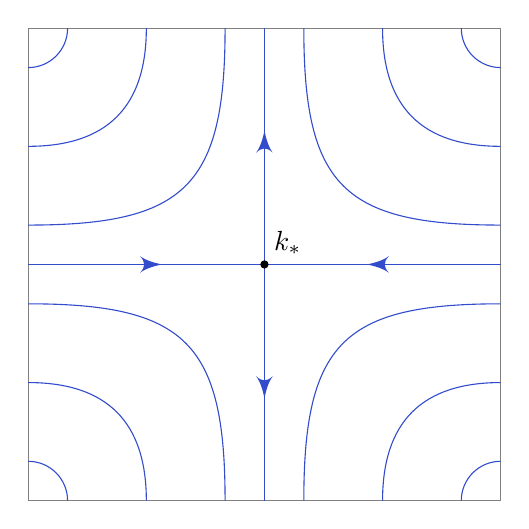
\begin{tikzpicture}
    \draw [gray] (-3, -3) rectangle (3, 3);

    \draw [mblue] (-3, 0) -- (3, 0);
    \draw [mblue] (0, -3) -- (0, 3);
    \node [circ] at (0 ,0) {};
    \node [anchor = south west] at (0, 0) {$k_*$};

    \foreach \x in {0,90,180,270} {
      \begin{scope}[rotate=\x]
        \draw [mblue] (0.5, -3) .. controls (0.5, -1) and (1, -0.5) .. (3, -0.5);
        \draw [mblue] (1.5, -3) .. controls (1.5, -2) and (2, -1.5) .. (3, -1.5);

        \draw [mblue] (2.5, -3) arc(180:90:0.5);
      \end{scope}
    }

    \draw [mblue, ->] (-1.3, 0) -- +(0.001, 0);
    \draw [mblue, ->] (1.3, 0) -- +(-0.001, 0);
    \draw [mblue, ->] (0, -1.7) -- +(0, -0.001);
    \draw [mblue, ->] (0, 1.7) -- +(0, 0.001);
  \end{tikzpicture}
\end{center}
where the arrows denote the direction of steepest descent of $\rho_r$. Note that since the real part satisfies Laplace's equation, such a stationary point must be a saddle, instead of a local maximum or minimum, even if the zero is not second-order.

We now see that if our start and end points lie on opposite sides of the ridge, i.e.\ one is below the horizontal line and the other is above, then the only way to do so while staying on a path of stationary phase is to go through the stationary point.

Along such a contour, we would expect the greatest contribution to the integral to occur when $\rho_r$ is the greatest, i.e.\ at $k_*$. We can expand $\rho$ about $k_*$ as
%
%Now there are many contours of $\rho_i$. Which of them should we pick? Along such contours, the greatest contribution comes from the point where $\rho_r(k)$ is the greatest. If we want to essentially approximate the whole integral by the value at the maximum, then we should pick a contour where $\rho_r(k)$ drops as quickly as possible when we move away from the maximum. After some work, we see that we should pick the contour that passes through the points $k_*$ with $\frac{\partial \rho}{\partial k}(k^*) = 0$.
%
%Note that since $\rho_r$ and $\rho_i$ satisfy Laplace's equation,
%
%
%To approximate the integral, we expand $\rho$ about the point $k_*$, to get
\[
  \rho(k) \sim \rho(k_*) + \frac{1}{2} \frac{\partial^2 \rho}{\partial k^2} (k_*) (k - k_*)^2.
\]
We can then approximate
\[
  H(t) \sim \frac{-i}{2\pi}\int_{\varepsilon} f(k) e^{t \rho(k)}\;\d k,
\]
where we are just integrating over a tiny portion of our contour near $k_*$. Putting in our series expansion of $\rho$, we can write this as
\[
  H(t) \sim \frac{-i}{2\pi} f(k_*) e^{t\rho(k_*)} \int_{\varepsilon} \exp\left(\frac{t}{2} \frac{\partial^2 \rho}{\partial k^2} (k_*) (k - k_*)^2\right)\;\d k.
\]
Recall that we picked our path to be the path of steepest descent on both sides of the ridge. So we can paramretrize our path by $K$ such that
\[
  (iK)^2 = \frac{t}{2} \frac{\partial^2 \rho}{\partial k^2} (k_*) (k - k_*)^2,
\]
where $K$ is purely real. So our approximation becomes
\[
  H(t) \sim \frac{f(k_*) e^{t \rho(k_*)}}{\sqrt{2\pi^2 t \rho''(k_*)}} \int_{-\varepsilon}^\varepsilon e^{-K^2}\;\d K.
\]
Since $e^{-K^2}$ falls of so quickly as $k$ gets away from $0$, we may approximate that integral by an integral over the whole real line, which we know gives $\sqrt{\pi}$. So our final approximation is
\[
  H(t) \sim \frac{f(k_*) e^{t \rho(k_*)}}{\sqrt{2\pi t \rho''(k_*)}}.
\]
We then look at the maxima of $\rho_r(k)$ along these paths and see which has the greatest contribution.

Now let's apply this to our situation. Our $\rho$ was given by
\[
  \rho(k) = i (kV - \omega(k)).
\]
So $k_*$ is given by solving
\[
  \frac{\partial \omega}{\partial k}(k_*) = V.\tag{$*$}
\]
Thus, what we have shown was that the greatest contribution to the Green's function along the $V$ direction comes from the the modes whose group velocity is $V$! Note that in general, this $k_*$ is complex.

Thus, the conclusion is that given any $V$, we should find the $k_*$ such that ($*$) is satisfied. The temporal growth rate along $\frac{x}{t} = V$ is then
\[
  \sigma(V) = \omega_i(k_*) - k_{*i}V.
\]
This is the growth rate we would experience if we moved at velocity $V$. However, it is often more useful to consider the absolute growth rate. In this case, we should try to maximize $\omega_i$. Suppose this is achieved at $k = k_{max}$, possibly complex. Then we have
\[
  \frac{\partial \omega_i}{\partial k}(k_{max}) = 0.
\]
But this means that $c_g = \frac{\partial \omega}{\partial k}$ is purely real. Thus, this maximally unstable mode can be realized along some physically existent $V = c_g$.


%
%Remember that $\rho = \rho_r + i \rho_i$ is complex and analytic. So $\rho_r$ and $\rho_i$ satisfy the Cauchy--Riemann equations
%\[
%  \frac{\partial \rho_r}{\partial k_r} = \frac{\partial \rho_i}{\partial k_i},\quad \frac{\partial \rho_r}{\partial k_i} = - \frac{\partial \rho_i}{\partial k_r}.
%\]
%In particular, we deduce that the gradients (with respect to $k$) are orthogonal: $\nabla_k \rho_r \cdot \nabla_k \rho_i = 0$. Also, $\rho_r$ and $\rho_i$ satisfy Laplace's equation
%\[
%  \nabla_k^2 \rho_r = \nabla_k^2 \rho_i = 0.
%\]
%Thus, we know that any critical point $k_*$ for $\rho$ must be a saddle point.
%
%We know that the integral is dominated by the largest value of $\rho_r$ in vicinity of $k_*$, where we can expand
%\[
%  \rho\left(k; \frac{x}{t}\right) \sim \rho\left(k_*; \frac{x}{t}\right) + \frac{1}{2} \frac{\partial^2}{\partial k^2} \rho\left(k_*; \frac{x}{t}\right)(k - k_*)^2.
%\]
%Since we are sitting on a complex plane, by Cauchy's thoerem, the value of the integral should be independent of the path. So we may distort the contour as we wish, and the trick is to follow the steepest descent for the real part. Then by orthogonality, we are \emph{guaranteed} that this is the direction of stationary phase!
%
%Now if we believe that the dominant contribution is due to what happens at $k_*$, then we can approximate
%\[
%  G(x, t) \sim \frac{-i}{2\pi} \left(f(k_*) \exp \left(t \rho \left(k_*; \frac{x}{t}\right)\right)\right) \int_{F_k} \exp \left(\frac{t}{2} \frac{\partial^2}{\partial k^2} \rho\left(k_*; \frac{x}{t}\right)(k - k_*)^2\right)\;\d k.
%\]
%We can substitute
%\[
%  (iK)^2 = \frac{t}{2} \frac{\partial^2}{\partial k^2}\rho\left(k_*; \frac{x}{t}\right)(k - k_*)^2.
%\]
%So we are left with
%\[
%  G(x, t) \sim \frac{f(k_*) \exp \left(t \rho\left(k_*; \frac{x}{t}\right)\right)}{ \sqrt{2\pi^2 t \frac{\partial^2}{\partial k^2} \rho(k_*; \frac{x}{t})}} \int_{-\infty}^\infty e^{-K^2}\;\d K = \frac{f(k_*) \exp \left((t \rho\left((k_*; \frac{x}{t}\right)\right)}{ \sqrt{2\pi t \frac{\partial^2}{\partial k^2} \rho(k_*; \frac{x}{t})}}
%\]
%Now recall that we had
%\[
%  \rho = i \left(k \left(\frac{x}{t}\right) - \omega(k)\right).
%\]
%So we simply have
%\[
%  \frac{\partial^2 \rho}{\partial k^2} = -i \frac{\partial^2 \omega}{\partial k^2}.
%\]
%So for an observer at $V = \frac{x}{t}$, we have
%\[
%  G(x, t) \sim \frac{e^{i\pi/4} e^{i(k_* x - \omega(k_*)t}}{\frac{\partial D}{\partial \omega}(k_*, \omega(k_*)) \sqrt{2\pi t \frac{\partial^2}{\partial k^2}\omega(k_*)}},
%\]
%and
%\[
%  \frac{\partial \omega}{\partial k}(k_*) = \frac{x}{t}.
%\]
%We then see that the temporal growth rate is
%\[
%  \sigma(V) = \omega_i(k_*) - k_{*i} V.
%\]
%Generically, we expect there is a maximum growth rate at some $k = k_{max}$. Then
%\[
%  \omega_i(k_{max}) = \omega_{i, max}.
%\]
%So we have
%\[
%  \frac{\partial \omega_i}{\partial k} (k_{max}) = 0.
%\]
%So it follows that the group velocity
%\[
%  c_g = \frac{\partial \omega}{\partial k}(k_{max}) = V_{max}
%\]
%is real, and is thus well-defined.

%Now if $\omega_{i, max} < 0$, then $\sigma(V) < 0$ for all $V = \frac{x}{t}$. So the flow is linearly stable.
%
%On the other hand, if $\omega_{i, max} > 0$, then $\sigma(V) > 0$ for all $V = \frac{x}{t}$. on the other hand, if $\omega_{i, max} > 0$, then it is linearly unstable.

We can now say
\begin{itemize}
  \item If $\omega_{i, max} < 0$, then the flow is linearly stable.
  \item If $\omega_{i, max} > 0$, then the flow is linearly unstable. In this case,
    \begin{itemize}
      \item If $\omega_{0, i} < 0$, then the flow is convectively unstable.
      \item If $\omega_{0, i} > 0$, then the flow is absolutely unstable.
    \end{itemize}
\end{itemize}
Here $\omega_0$ is defined by first solving $\frac{\partial \omega}{\partial k}(k_0) = 0$, thus determining the $k_0$ that leads to a zero group velocity, and then setting $\omega_0 = \omega(k_0)$. These quantities are known as the \term{absolute frequency} and \term{absolute growth rate} respectively.

%For the convective/absolute issue, we can consider the (complex) \term{absolute wavenumber} $k_0$ defined by
%\[
%  \frac{\partial \omega}{\partial k}(k_0) = 0.
%\]
%There is an associated (complex) \term{absolute frequency} and \term{absolute growth rate} $\omega_0 = \omega(k_0)$ and $\sigma(0) = \omega_{0, i}$.
%
%Therefore we can obtain the Briggs--Bers criterion for unstable flows: if $\omega_{_0, i} < 0$, then the flow is convectively unstable, and if $0 < V_- < V_+$. If $\omega_{0,i} > 0$, then the flow is absolutely unstable and $V_i < 0 < V_+$.
%
\begin{eg}
  We can consider a ``model dispersion relation'' given by the \term{linear complex Ginzburg--Landau equation}
  \[
    \left(\frac{\partial}{\partial t} + U \frac{\partial}{\partial x}\right) \chi - \mu \chi - (1 + i c_d) \frac{\partial^2}{\partial x^2}\chi = 0.
  \]
  This has advection ($U$), dispersion ($c_d$) and instability ($\mu$). Indeed, if we replace $\frac{\partial}{\partial t} \leftrightarrow -i\omega$ and $\frac{\partial}{\partial x} \leftrightarrow ik$, then we have
  \[
    i(-\omega + Uk)\chi - \mu \chi + (1 + ic_d) k^2 \chi = 0.
  \]
  This gives
  \[
    \omega = Uk + c_d k^2 + i(\mu - k^2).
  \]
  We see that we have temporal instability for $|k| < \sqrt{\mu}$, where we assume $\mu > 0$. This has
  \[
    c_r = \frac{\omega_r}{k} = U + c_d k.
  \]
  On the other hand, if we force $\omega \in \R$, then we have spatial instability. Solving
  \[
    k^2 (c_d - i) + Uk + (i\mu - \omega) = 0,
  \]
  the quadratic equation gives us two branches
  \[
    k^{\pm} = \frac{-U \pm \sqrt{k^2 - 4(i\mu - \omega)(c_d - i)}}{2(c_d - i)}.
  \]
  To understand whether this instability is convective or absolute, we can complete the square to obtain
  \[
    \omega = \omega_0 + \frac{1}{2} \omega_{kk}(k - k_0)^2,
  \]
  where
  \begin{align*}
    \omega_{kk} &= 2(c_d - i)\\
    k_0 &= \frac{U}{2(i - c_d)}\\
    \omega_0 &= -\frac{c_d U^2}{4(1 + c_d^2)} +i \left(\mu - \frac{U^2}{4(1 + c_d^2)}\right).
  \end{align*}
  These $k_0$ are then the absolute wavenumber and absolute frequency. % interplay between advection and dispersion
\end{eg}

%Inverting this relation, we can write
%\[
%  k^{\pm}(\omega) = k_0 \pm \left(\frac{2}{\omega_{kk}}\right)^{1/2} (\omega - \omega_0)^{1/2}.
%\]
Note that after completing the square, it is clera that $k_0$ is a double root at $\omega = \omega_0$. Of course, there is not nothing special about this example, since $k_0$ was defined to solve $\frac{\partial \omega}{\partial k}(k_0) = 0$!

I really ought to say something about Bers' method at this point.

%In 1983, Bers identified a geometric method to find $\omega_0, k_0$ --- we find \term{pinch points} as $L_\omega$ is lowered.
%
%Indeed, for each fixed $\omega_i$, the contour $L_\omega$ generically corresponds to two branches $k^{\pm}(L_\omega)$ in $k$ space as dictated by the dispersion relation. Conversely, the contour $F_k$ for a fixed $k_i$ corresopnds to a branch $\omega(F_k)$ in $\omega$ space.
%
%% insert picture
%
%By causlity, it must be the case that $\omega(F_k)$ lies below $L_\omega$, and $F_k$ lies in between $k^{\pm}(L_\omega)$.

In practice, it is not feasible to apply a $\delta$ function of perturbation and see how it grows. Instead, we can try to understand convective versus absolute instabilities using a periodic and switched on forcing
\[
  F(x, t) = \delta(x) H(t) e^{-i\omega_f t},
\]
where $H$ is the Heaviside step function. The response in spectral space is then
\[
  \tilde{\chi}(k, \omega) = \frac{\tilde{F}(k, \omega)}{D(k, \omega)} = \frac{i}{D(k, \omega)(\omega - \omega_f)}.
\]
There is a new (simple) pole precisely at $\omega = \omega_f$ on the real axis. We can invert for $t$ to obtain
\[
  \tilde{\chi}(k, t) = \frac{i}{2\pi} \int_{L_\omega} \frac{e^{-i\omega t}}{D(k, \omega) (\omega - \omega_F)}\;\d \omega = \frac{e^{-i\omega_f t}}{D(k, \omega_f)} + \frac{e^{-i\omega(k) t}}{(\omega(k) - \omega_f) \frac{\partial \tilde{D}}{\partial \omega}[k, \omega(k)]}.
\]
We can then invert for $x$ to obtain
\[
  \chi(x, t) = \underbrace{\frac{e^{-i\omega_f t}}{2\pi} \int_{F_k} \frac{e^{ikx}}{D(k, \omega)}\;\d k}_{\chi_F(x, t)} + \underbrace{\frac{1}{2\pi} \int_{F_k} \frac{e^{i[kx - \omega(k) t]}}{[\omega(k) - \omega_f] \frac{\partial \tilde{D}}{\partial \omega} [k, \omega(k)]}}_{\chi_T(x, t)}.
\]
The second term is associated with the switch-on transients, and is very similar to what we get in the previous steepest descent.

If the flow is absolutely unstable, then the transients dominate and invade the entire domain. But if the flow is convectively unstable, then this term is swept away, and all that is left is $\chi_F(x, t)$. This gives us a way to distinguish between

Note that in the forcing term, we get contributions at the singularities $k^{\pm}(\omega_f)$. Which one contributes depends on causality. One then checks that the correct result is
\[
  \chi_F(x, t) = iH(x) \frac{e^{i(k^+(\omega_f)x - \omega_f t)}}{\frac{\partial D}{\partial k} [k^+(\omega_f), \omega_f]} - i H(-x) \frac{e^{i(k^-(\omega_f) x - \omega_f t)}}{\frac{\partial D}{\partial k} [k^-(\omega_f), \omega_f]}.
\]
Note that $k^{\pm}(\omega_f)$ may have imaginary parts! If there is some $\omega_f$ such that $-k_i^+(\omega_f) > 0$, then we will see spatially growing waves in $x > 0$. Similarly, if there exists some $\omega_f$ such that $-k_i^-(\omega_f) < 0$, then we see spatially growing waves in $x < 0$.

Note that we will see this effect only when we are convectively unstable.

%We can plot the GLE branches of $k^+(\omega)$ and $k^-(\omega)$ branches, which are valid for the convectively unstable regime
%\[
%  0 \leq \mu \leq \frac{U^2}{4 (1 + c_d^2)}.
%\]
%% insert picture
%
Perhaps it is wise to apply these ideas to an actual fluid dynamics problem. We revisit the broken line shear layer profile, scaled with the velocity jump, but allow a non-zero mean $U$:
\begin{center}
  \begin{tikzpicture}
    \draw [dashed] (-2, -1) -- (2, -1) node [right] {$z = 1$};

    \draw [dashed] (-2, 1) -- (2, 1) node [right] {$z = -1$};
    \draw (-1, -3) -- (-1, -1) node [pos=0.5, right] {$\bar{U} = -1 + U_m$} -- (1, 1) node [pos=0.5, right] {$\bar{U} = z + U_m$} -- (1, 3) node [pos=0.5, right] {$\bar{U} = 1 + U_m$};
    \node at (-2, -2) {III};
    \node at (-2, 0) {II};
    \node at (-2, 2) {I};

    \node [right] at (3.5, 2) {$Ae^{-\alpha(z - 1)}$};
    \node [right] at (3.5, 0) {$Be^{\alpha z} + Ce^{-\alpha z}$};
    \node [right] at (3.5, -2) {$D e^{\alpha (z + 1)}$};
  \end{tikzpicture}
\end{center}
We do the same interface matching conditions, and after doing the same computations (or waving your hands with Galilean transforms), we get the dispersion relation
\[
  4 (\omega - U_m \alpha)^2 = (2\alpha - 1)^2 - e^{-4\alpha}.
\]
It is now more natural to scale with $U_m$ rather than $\Delta U/2$, and this involves expressing everything in terms of the velocity ratio $R = \frac{\Delta U}{2 U_m}$. Then we can write the dispersion relation as
\[
  D(k, \omega; R) = 4(\omega - k)^2 - R^2[(2k - 1)^2 - e^{-4k}] = 0.
\]
Note that under this scaling, the velocity for $z < -1$ is $u = 1 - R$. In particular, if $R < 1$, then all of the fluid is flowing in the same direction, and we might expect the flow to ``carry away'' the perturbations, and this is indeed true.

The absolute/convective boundary is given by the frequency at wavenumber for zero group velocity:
\[
  \frac{\omega}{\partial k}(k_0) = 0.
\]
This gives us
\[
  \omega_0 = k_0 - \frac{R^2}{2} [2k_0 - 1 + e^{-4k_0}].
\]
Plugging this into the dispersion relations, we obtain
\[
  R^2 [2k_0 - 1 + e^{-4k_0}] - [(2k_0 -1 )^2 - e^{-4k_0}] = 0.
\]
We solve for $k_0$, which is in general \emph{complex}, and then solve for $\omega$ to see if it leads to $\omega_{0, i} > 0$. This has to be done numerically, and when we do this, we see that the convective/absolute boundary occurs precisely at $R = 1$.

\subsubsection*{Gaster relation}
Temporal and spatial instabilities are related close to a marginally stable state. This is flow at a critical parameter $R_c$ with critical (real) wavenumber and frequency: $D(k_c, \omega_c; R_c) = 0$ with $\omega_{c, i} = k_{c, i} = 0$.

We can Taylor expand the dispersion relation
\[
  \omega = \omega_c + \frac{\partial \omega}{\partial k} (k_c; R_c) [k - k_c].
\]
We take the imaginary part
\[
  \omega_i = \frac{\partial \omega_i}{\partial k_r} (k_c, R_c) (k_r - k_c) + \frac{\partial \omega_r}{\partial k_r}(k_c, R_c)k_i.
\]
For the temporal mode, we have $k_i = 0$, and so
\[
  \omega_i^{(T)} = \frac{\partial \omega_i}{\partial k_r}(k_c, R_c)(k_r - k_c).
\]
For the spatial mode, we have $\omega_i = 0$, and so
\[
  0 = \frac{\partial \omega_i}{\partial k_r}(k_c, R_c)[k_r - k_c] + \frac{\partial \omega_r}{\partial k_r} (k_c, R_c)k_i^{(S)}.
\]
Remembering that $c_g = \frac{\partial \omega_r}{\partial k_r}$. So we find that
\[
  \omega_i^{(T)} = - c_g k_i^{(S)}.
\]
This gives us a relation between the growth rates of the temporal mode and spatial mode when we are near the marginal stable state.

Bizarrely, this is often a good approximation when we are \emph{far} from the marginal state.

\subsubsection*{Global instabilities}
So far, we have always been looking at flows that were parallel, i.e.\ the base flow depends on $z$ alone. However, in real life, flows tend to evolve downstream. Thus, we want to consider base flows $U = U(x, z)$.

Let $\lambda$ be the characteristic wavelength of the perturbation, and $L$ be the characteristic length of the change in $U$. If we assume $\varepsilon \sim \frac{\lambda}{L} \ll 1$, then we may want to perform some local analysis.

To leading order in $\varepsilon$, evolution is governed by \emph{frozen} dispersion relation at each $X = \varepsilon x$. We can then extend notions of stability/convective/absolute to local notions, e.g.\ a flow is locally convectively unstable if there is some $X$ such that $\omega_{i, max}(X) > 0$, but $\omega_{0, i}(X) < 0$ for all $X$.

However, we can certainly imagine some complicated interactions between the different region. For example, a perturbation upstream may be swept downstream by the flow, and then get ``stuck'' somewhere down there. In general, we can define

%% discuss patch of instability in locally absolutely unstable
%
%The WKBJ analysis can follow our previous approach. We can consider the impulse resupose
%\[
%  \left[ D (-\partial_x, i \partial_t; X) + \varepsilon \D_\varepsilon (-i \partial_x, i \partial_t; X)\right] G(x, t) = \delta(x) \delta(t),
%\]
%where $X = \varepsilon x$.
%
%Now $X$ is not frozen, and we can define new concepts of stability:
\begin{defi}[Global stability]\index{global stability}
  A flow is \emph{globally stable} if $\lim_{t \to \infty} G(x, t) = 0$ for all $x$.

  A flow is \emph{globally unstable} if there is some $x$ such that $\lim_{t \to \infty} G(x, t) \to \infty$.
\end{defi}

For a steady spatially developing flow, global modes are
\[
  \chi(x, t) = \phi(x) e^{-i \omega_G t}.
\]
The complex global frequency $\omega_G$ is determined analogously to before using complex integration.

It can be established that $\omega_{G, i} \leq \omega_{0, i, max}$. This then gives a necessary condition for global instability: there must be a region of local absolute instability within the flow.

Sometimes this is a good predictor, i.e.\ $R_{G_c} \simeq R_t$. For example, with mixing layers, we have $R_t = 1.315$ while $R_{G_c} = 1.34$. On the other hand, it is sometimes poor. For example, for bluff-body wakes, we have $Re_t = 25$ while $Re_{Gc} = 48.5$.

\section{Transient growth}
\subsection{Motivation}
So far, our model of stability is quite simple. We linearize our theory, look at the individual perturbation modes, and say the system is unstable if there is exponential growth. In certain circumstances, it works quite well. In others, they are just completely wrong.

There are six billion kilometers of pipes in the United States alone, where the flow is turbulent. A lot of energy is spent pumping fluids through these pipes, and turbulence is not helping. So we might think we should try to understand flow in a pipe mathematically, and see if it gives ways to improve the situation.

Unfortunately, we can prove that flow in a pipe is linearly stable for all Reynolds numbers. The analysis is not \emph{wrong}. The flow is indeed linearly stable. The real problem is that linear stability is not the right thing to consider.

%In reality, we find that turbulence starts to occur for
%\[
%  Re = \frac{QD}{\nu A} \sim 2000.
%\]
%If we On the other hand, this can be avoided for a quiet flow for $Re \sim 10^5$. What is going on?

We get similar issues with plane Poiseuille flow, i.e.\ a pressure driven flow between horizontal plates. As we know from IB Fluids, the flow profile is a parabola:
\begin{center}
  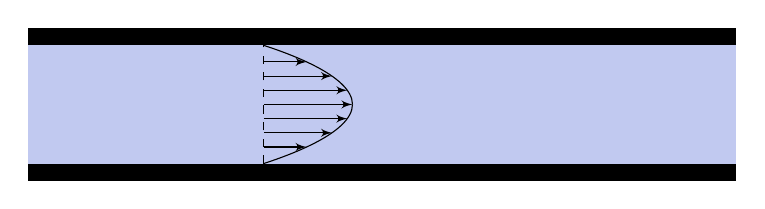
\begin{tikzpicture}[scale=1.5]
    \fill [black] (0, 0) rectangle (6, -0.15);
    \fill [black] (0, 1) rectangle (6, 1.15);
    \fill [opacity=0.3, mblue] (0, 0) rectangle (6, 1);

    \foreach \x in {0.14, 0.26, 0.38, 0.5, 0.62, 0.74, 0.86} {
      \pgfmathsetmacro\len{\x * (1 - \x)}
      \draw [-latex'] (2, \x) -- +(3 * \len, 0);
    };
    \draw [rotate=270, yscale=-1, shift={(-3,-3)}] (2.5, 0.25) parabola (2, 1);% magic
    \draw [rotate=90, shift={(-2,-3)}] (2.5, 0.25) parabola (2, 1);
    \draw [dashed] (2, 0) -- (2, 1);
  \end{tikzpicture}
\end{center}
One can analyze this and prove that it is linearly unstable when
\[
  Re = \frac{U_c d}{\nu} > 5772.
\]
However, it is observed to be unstable at much lower $Re$.

We have an even more extreme issue for plane Couette flow. This is flow between two plates at $z = \pm 1$ (after rescaling) driven at speeds of $\pm 1$ (after scaling). Thus, the base flow is given by
\[
  \bar{U} = z,\quad |z| \leq 1.
\]
Assuming the fluid is inviscid, the Rayleigh equation then tells us perturbations obey
\[
  \left[ (\bar{U} - c) \left(\frac{\d^2}{\d z^2} - k^2\right) - \frac{\d^2}{\d z^2} \bar{U} \right] \hat{w} = 0.
\]
Since $\bar{U} = z$, the second derivative term drops out and this becomes
\[
  (\bar{U} - c) \left(\frac{\d^2}{\d z^2} - k^2\right) \hat{w} = 0.
\]
If we want our solution to be smooth, or even just continuously differentiable, then we need $\left(\frac{\d^2}{\d z^2} - k^2\right) \hat{w} = 0$. So the solution is of the form
\[
  \hat{w} = A \sinh k(z + 1) + B \sinh k(z - 1).
\]
However, to satisfy the boundary conditions $\hat{w}(\pm 1) = 0$, then we must have $A = B = 0$, i.e.\ $\hat{w} = 0$.

Of course, it is \emph{not} true that there can be no perturbations. Instead, we have to relax the requirement that the eigenfunction is smooth. We shall allow it to be non-differentiable at certain points, but still require that it is continuous (alternatively, we relax differentiability to weak differentiability).

The fundamental assumption that the eigenfunction is smooth must be relaxed. Let's instead consider a solution of the form
\begin{align*}
  \hat{w}_+ &= A_+ \sinh k (z - 1) & z &> z_c\\
  \hat{w}_- &= A_- \sinh k(z + 1) & z &< z_c.
\end{align*}
If we require the vertical velocity to be continuous at the critical layer, then we must have the matching condition
\[
  A_+ \sinh k (z - z_c) = A_- \sinh k(z + z_c).
\]
This still satisfies the Rayleigh equation if $\bar{U} = c$ at the critical layer. Note that $u$ is discontinuous at the critical layer, because incompressibility requires
\[
  \frac{\partial w}{\partial z} = - \frac{\partial u}{\partial x} = -iku.
\]
\begin{center}
  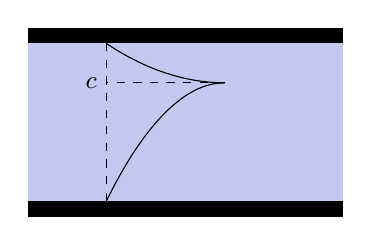
\begin{tikzpicture}
    \fill [black] (0, 0) rectangle (4, -0.2);
    \fill [black] (0, 2) rectangle (4, 2.2);
    \fill [opacity=0.3, mblue] (0, 0) rectangle (4, 2);

    \draw [dashed] (1, 0) -- (1, 2);

    \draw (2.5, 1.5) parabola (1, 0);
    \draw (2.5, 1.5) parabola (1, 2);

    \draw [dashed] (2.5, 1.5) -- (1, 1.5) node [left] {\small$c$};
  \end{tikzpicture}
\end{center} % improve this picture
So for all $|c| = |\omega/k| < 1$, there is a (marginally stable) mode. The spectrum is \emph{continuous}. There is no discrete spectrum. This is quite weird, compared to what we have previously seen.

But still, we have only found modes with a real $c$, since $\bar{U}$ is real! Thus, we conclude that inviscid plane Couette flow is stable! While viscosity regularizes the flow, but it turns out that does not linearly destabilize the flow at \emph{any} Reynolds number (Romanov, 1973).

Experimentally, and numerically, plane Couette flow is known to exhibit a rich array of dynamics.
\begin{itemize}
  \item Up to $Re \approx 280$, we have laminar flow.
  \item Up to $Re \approx 325$, we have transient spots.
  \item Up to $Re \approx 415$, we have sustained spots and stripes.
  \item For $Re > 415$, we have fully-developed turbulence.
\end{itemize}
In this chapter, we wish to understand transient growth. This is the case when small perturbations can grow up to some visible, significant size, and then die off.

\subsection{A toy model}
Let's try to understand transient dynamics in a finite-dimensional setting. Ultimately, the existence of transient growth is due to the \emph{non-normality} of the operator.

Recall that a matrix $A$ is \emph{normal}\index{normal operator} iff $A^\dagger A = A A^\dagger$. Of course, self-adjoint matrices are examples of normal operators. The spectral theorem says a normal operator has a complete basis of orthonormal eigenvectors, which is the situation we understand well. However, if our operator is not normal, then we don't necessarily have a basis of eigenvectors, and even if we do, they need not be orthonormal.

So suppose we are in a $2$-dimensional world, and we have two eigenvectors that are very close to each other:
\begin{center}
  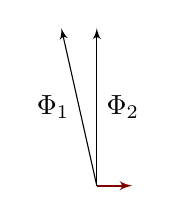
\begin{tikzpicture}[xscale=1.5]
    \draw [-latex'] (0, 0) -- (0, 2) node [pos=0.5, right] {$\Phi_2$};
    \draw [-latex'] (0, 0) -- (-0.3, 2) node [pos=0.5, left] {$\Phi_1$};

    \draw [-latex', mred, semithick] (0, 0) -- (0.3, 0);
  \end{tikzpicture}
\end{center}
Now suppose we have a small perturbation given by $\boldsymbol\varepsilon = (\varepsilon, 0)^T$. While this perturbation is very small in magnitude, if we want to expand this in the basis $\Phi_1$ and $\Phi_2$, we must use coefficients that are themselves quite large. In this case, we might have $\boldsymbol\varepsilon = \Phi_2 - \Phi_1$, as indicated in red in the diagram above.

Let's let this evolve in time. Suppose both $\Phi_1$ and $\Phi_2$ are stable modes, but $\Phi_1$ decays much more quickly than $\Phi_2$. Then after some time, the perturbation will grow like
\begin{center}
  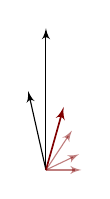
\begin{tikzpicture}[xscale=1.5]
    \draw [-latex'] (0, 0) -- (0, 1.8);
    \draw [-latex'] (0, 0) -- (-0.15, 1);

    \draw [-latex', mred, semithick] (0, 0) -- (0.15, 0.8);
    \draw [-latex', mred, opacity=0.5] (0, 0) -- (0.22, 0.5);
    \draw [-latex', mred, opacity=0.5] (0, 0) -- (0.28, 0.2);
    \draw [-latex', mred, opacity=0.5] (0, 0) -- (0.3, 0);
  \end{tikzpicture}
\end{center}
Note that the perturbation grows to reach a finite, large size, until it vanishes again as the $\Phi_1$ component goes away.

Let's try to put this down more concretely in terms of equations. We shall consider a linear ODE of the form
\[
  \dot{\mathbf{x}} = A \mathbf{x}.
\]
We first begin by considering the matrix
\[
  A =
  \begin{pmatrix}
    0 & 1\\
    0 & 0
  \end{pmatrix},
\]
which does \emph{not} exhibit transient growth. We first check that $A$ is not normal. Indeed,
\[
  AA^T
  \begin{pmatrix}
    1 & 0\\
    0 & 0
  \end{pmatrix} \not=
  \begin{pmatrix}
    0 & 0\\
    0 & 1
  \end{pmatrix} = A^T A.
\]
Note that the matrix $A$ has a repeated eigenvalue of $0$ with a \emph{single} eigenvector of $(1\; 0)$.

To solve this system, write the equations more explicitly as
\begin{align*}
  \dot{x}_1 &= x_2\\
  \dot{x_2} &= 0.
\end{align*}
If we impose the initial condition
\[
  (x_1, x_2)(0) = (x_{10}, x_{20}),
\]
then the solution is
\begin{align*}
  x_1(t) &= x_{20}t + x_{10}\\
  x_2(t) &= x_{20}.
\end{align*}
This exhibits linear, algebraic growth instead of the familiar exponential growth.

Let's imagine we perturb this system slightly. We can think of our previous system as the $Re = \infty$ approximation, and this small perturbation as the effect of a large but finite Reynolds number. For $\varepsilon > 0$, set
\[
  A_\varepsilon =
  \begin{pmatrix}
    -\varepsilon & 1\\
    0 & -2\varepsilon
  \end{pmatrix}.
\]
We then have eigenvalues
\begin{align*}
  \lambda_1 &= -\varepsilon\\
  \lambda_2 &= -2\varepsilon,
\end{align*}
corresponding to eigenvectors
\[
  \mathbf{e}_1 =
  \begin{pmatrix}
    1 \\0
  \end{pmatrix},\quad \mathbf{e}_2 =
  \begin{pmatrix}
    1 \\\ -\varepsilon
  \end{pmatrix}.
\]
Notice that the system is now stable. However, the eigenvectors are very close to being parallel.

As we previously discussed, if we have an initial perturbation $(\varepsilon, 0)$, then it is expressed in this basis as $e_1 - e_2$. As we evolve this in time, the $e_2$ component decays more quickly than $e_1$. So after some time, the $e_2$ term is mostly gone, and what is left is a finite multiple of $e_1$, and generically, we expect this to have magnitude larger than $\varepsilon$!

We try to actually solve this. The second row in $\dot{\mathbf{x}} = A\mathbf{x}$ gives us
\[
  \dot{x}_2 = -2\varepsilon x_2.
\]
This is easy to solve to get
\[
  x_2 = x_{20} e^{-2\varepsilon t}.
\]
Plugging this into the first equation, we have
\[
  \dot{x}_1 = -\varepsilon x_1 + x_{20} e^{-2\varepsilon t}.
\]
We would expect a solution of the form $x_1 = A e^{-\varepsilon t} - B e^{-2 \varepsilon t}$, where the first term is the homogeneous solution and the second comes from a particular solution. Plugging this into the equation and applying our initial conditions, we need
\[
  x_1 = \left(x_{10} + \frac{x_{20}}{\varepsilon}\right) e^{-\varepsilon t} - \frac{x_{20}}{\varepsilon} e^{-2 \varepsilon t}.
\]
Let us set
\begin{align*}
  y_{10} &= x_{10} + \frac{x_{20}}{\varepsilon}\\
  y_{20} &= -\frac{x_{20}}{\varepsilon}.
\end{align*}
Then the full solution is
\[
  \mathbf{x} = y_{10} e^{-\varepsilon t} \mathbf{e}_1 + y_{20} e^{-2\varepsilon t} \mathbf{e}_2.
\]
For $\varepsilon t \gg 1$, we know that $\mathbf{x} \sim y_{10} e^{-\varepsilon t} \mathbf{e}_2$. So our solution is an exponentially decaying solution.

But how about early times? Let's consider the magnitude of $x$. We have
\begin{align*}
  \|\mathbf{x}\|^2 &= y_{10}^2 e^{-2 \varepsilon t} \mathbf{e}_1 \cdot \mathbf{e}_2 + 2y_{10} y_{20} e^{-3\varepsilon t} \mathbf{e}_1 \cdot \mathbf{e}_2 + y_{20}^2 e^{-4\varepsilon t} \mathbf{e}_2 \mathbf{e}_2\\
  &= y_{10}^2 e^{-2\varepsilon t} + 2y_{10} y_{20} e^{-3 \varepsilon t} + (1 + \varepsilon^2) y_{20}^2 e^{-4 \varepsilon t}.
\end{align*}
If $y_{10} = 0$ or $y_{20} = 0$, then this corresponds to pure exponential decay.

Thus, consider the situation where $y_{20} = - a y_{10}$ for $a \not =0$. Doing some manipulations, we find that
\[
  \|\mathbf{x}\|^2 = y_{10}^2 (1 - 2a + a^2 (1 + \varepsilon^2)) + y_{10}^2 (-2 + 6a - 4a^2(1 + \varepsilon^2))\varepsilon t + O(\varepsilon^2 t^2).
\]
Therefore we have initial growth if
\[
  4a^2 (1 + \varepsilon^2) - a + 2 < 0.
\]
Equivalently, if
\[
  a_- < a < a_+
\]
with
\[
  a_{\pm} = \frac{3 \pm \sqrt{1 - 8\varepsilon^2}}{4(1 + \varepsilon^2)}.
\]
Expanding in $\varepsilon$, we have
\begin{align*}
  a_+ &= 1 - 2 \varepsilon^2 + O(\varepsilon^4),\\
  a_- &= \frac{1 + \varepsilon^2}{2} + O(\varepsilon^4).
\end{align*}
These correspond to $s_{20} \simeq \frac{x_{10}}{2\varepsilon}$ and $x_{20} \simeq \varepsilon x_{10}$ respectively, for $\varepsilon \ll 1$. This is interesting, since in the first case, we have $x_{20} \gg x_{10}$, while in the second case, we have the opposite. So this covers a wide range of possible $x_{10}, x_{20}$.

What is the best initial condition to start with if we want the largest possible growth? Let's write everything in terms of $a$ for convenience, so that the energy is given by
\[
  E = \frac{\mathbf{x} \cdot \mathbf{x}}{2} = \frac{y_{10}^2}{2} (e^{-2\varepsilon t} - 2 a e^{-3 \varepsilon t} + a^2(1 + \varepsilon^2) e^{-4\varepsilon t}).
\]
Take the time derivative of this to get
\[
  \frac{\d E}{\d t} = - \varepsilon \frac{y_{10}^2}{2} e^{-2\varepsilon t} (2 - 6 (a e^{-\varepsilon t}) + 4 (1 + \varepsilon^2) (ae^{-\varepsilon t})^2).
\]
Setting $\hat{a} = ae^{-\varepsilon t}$, we have $\frac{\d E}{\d t} > 0$ iff
\[
  2 - 6 \hat{a} + 4 \hat{a}^2 (1 + \varepsilon^2) < 0.
\]
When $t = 0$, then $\hat{a} = a$, and we saw that there is an initial growth if $a_- < a < a_+$. We now see that we continue to have growth as long as $\hat{a}$ lies in this region. To see when $E$ reaches a maximum, we set $\frac{\d E}{\d t} = 0$, and so we have
\[
  (a_- - ae^{-\varepsilon t})(ae^{-\varepsilon t} - a_+) = 0.
\]
So a priori, this may happen when $\hat{a} = a_-$ or $a_+$. However, we know it must occur when $\hat{a}$ hits $a_-$, since $\hat{a}$ is decreasing with time. Call the time when this happens $t_{max}$, which we compute to be given by
\[
  \varepsilon t_{max} = \log \frac{a}{a_-}.
\]
Now consider the energy gain
\[
  G = \frac{E(t_{max})}{E(0)} = \frac{a_-^2}{a^2} \frac{a_-^2(1 + \varepsilon^2) - 2a_1 + 1}{a^2 (1 + \varepsilon^2) - 2a + 1}.
\]
Setting $\frac{\d G}{\d a} = 0$, we find that we need $a = a_+$, and so
\[
  \max_a G = \frac{(3a_- - 1)(1 - a_-)}{(3a_+ - 1)(1 - a_+)}.
\]
% use time translation invariance to argue this must be the case.

We can try to explicitly compute the value of the maximum energy gain, using our first-order approximations to $a_{\pm}$;
\[
  \max_a G = \frac{\left(3 \left(\frac{1 + \varepsilon^2}{2}\right)\right)\left(1 - \frac{1 + \varepsilon^2}{2}\right)}{(3(1 + 2\varepsilon^2) - 1)(1 - (1 - 2 \varepsilon^2))} = \frac{(1 + 3 \varepsilon^2)(1 - \varepsilon^2)}{16(1 - 3 \varepsilon^2)\varepsilon^2} \sim \frac{1}{16 \varepsilon^2}.
\]
So we see that we can have very large transient growth for a small $\varepsilon$.

How about the case where there is an unstable mode? We can consider a perturbation of the form
\[
  A =
  \begin{pmatrix}
    \varepsilon_1 & 1\\
    0 & -\varepsilon_2
  \end{pmatrix},
\]
with eigenvectors
\[
  \mathbf{e}_1 =
  \begin{pmatrix}
    1 \\0
  \end{pmatrix},\quad
  \mathbf{e}_2 = \frac{1}{\sqrt{1 + (\varepsilon_1 + \varepsilon_2)^2}}
  \begin{pmatrix}
    1\\
     -(\varepsilon_1 + \varepsilon_2)
  \end{pmatrix}
\]
We then have one growing mode and another decaying mode. Again, we have two eigenvectors that are very close to being parallel. We can do very similar computations, and see that what this gives us is the possibility of a large initial growth despite the fact that $\varepsilon_1$ is very small. In general, this growth scales as $\frac{1}{1 - \mathbf{e}_1 \cdot \mathbf{e}_2}$.

\subsection{A general mathematical framework}
Let's try to put this phenomenon in a general framework, which would be helpful since the vector spaces we deal with in fluid dynamics are not even finite-dimensional. Suppose $\mathbf{x}$ evolves under an equation
\[
  \dot{\mathbf{x}} = A \mathbf{x}.
\]
Given an inner product $\bra \ph, \ph\ket$ on our vector space, we can define the \term{adjoint} of $A$ by requiring
\[
  \bra \mathbf{x}, A\mathbf{y}\ket = \bra A^\dagger \mathbf{x}, \mathbf{y}\ket
\]
for all $x, y$. To see why we should care about the adjoint, note that in our previous example, the optimal perturbation came from an eigenvector of $A^\dagger$ for $\lambda_1 = \varepsilon$, namely $\begin{pmatrix} \varepsilon_1 + \varepsilon_2 \\ 1 \end{pmatrix}$ and we might conjecture that this is a general phenomenon.

For our purposes, we assume $A$ and hence $A^\dagger$ have a basis of eigenvectors. First of all, observe that the eigenvalues of $A$ are the complex conjugates of the eigenvalues of $A^\dagger$. Indeed, let $\mathbf{v}_1, \ldots, \mathbf{v}_n$ be a basis of eigenvectors of $A$ with eigenvalues $\lambda_1, \ldots, \lambda_n$, and $\mathbf{w}_1, \ldots, \mathbf{w}_n$ a basis of eigenvectors of $A^\dagger$ with eigenvalues $\mu_1, \ldots, \mu_n$. Then we have
\[
  \lambda_j \bra \mathbf{w}_i, \mathbf{v}_j\ket = \bra \mathbf{w}_i, A \mathbf{v}_j\ket = \bra A^\dagger \mathbf{w}_i, \mathbf{v}_j\ket = \mu_i^* \bra \mathbf{w}_i, \mathbf{v}_j\ket.
\]
But since the inner product is non-degenerate, for each $i$, it cannot be that $\bra \mathbf{w}_i, \mathbf{v}_j\ket = 0$ for all $j$. So there must be some $j$ such that $\lambda_j = \mu_i^*$.

By picking appropriate basis for each eigenspace, we can arrange the eigenvectors so that $\bra \mathbf{w}_i, \mathbf{v}_j\ket = 0$ unless $i = j$, and $\|\mathbf{w}_i\| = \|\mathbf{v}_j\| = 1$. This is the \term{biorthogonality property}. Crucially, the basis is \emph{not} orthonormal.

Now if we are given an initial condition $\mathbf{x}_0$, and we want to solve the equation $\dot{\mathbf{x}} = A\mathbf{x}$. Note that this is trivial to solve if $\mathbf{x}_0 = \mathbf{v}_j$ for some $j$. Then the solution is simply
\[
  \mathbf{x} = e^{\lambda_j t} \mathbf{v}_j.
\]
Thus, for a general $\mathbf{x}_0$, we should express $\mathbf{x}_0$ as a linear combination of the $\mathbf{v}_j$'s. If we want to write
\[
  \mathbf{x}_0 = \sum_{i = 1}^k \alpha_i \mathbf{v}_i,
\]
then using the biorthogonality condition, we should set
\[
  \alpha_i = \frac{\bra \mathbf{x}_0, \mathbf{w}_i\ket}{\bra \mathbf{v}_i, \mathbf{w}_i\ket}.
\]
Note that since we normalized our eigenvectors so that each eigenvector has norm $1$, the denominator $\bra \mathbf{v}_i, \mathbf{w}_i\ket$ can be small, hence $\alpha_i$ can be large, even if the norm of $\mathbf{x}_0$ is quite small, and as we have previously seen, this gives rise to transient growth if the eigenvalue of $\mathbf{v}_i$ is also larger than the other eigenvalues.

In our toy example, our condition for the existence of transient growth is that we have two eigenvectors that are very close to each other. In this formulation, the requirement is that $\bra \mathbf{v}_i, \mathbf{w}_i\ket$ is very small, i.e.\ $\mathbf{v}_i$ and $\mathbf{w}_i$ are close to being orthogonal. But these are essentially the same, since by the biorthogonality conditions, $\mathbf{w}_i$ is normal to all other eigenvectors of $A$. So if there is some eigenvector of $A$ that is very close to $\mathbf{v}_i$, then $\mathbf{w}_i$ must be very close to being orthogonal to $\mathbf{v}_i$.

%In our actual fluid dynamics problems, our spaces are infinite-dimensional. Note that if we want to sensibly talk about the ``size'' of the growth, and eigenvectors being ``close to parallel'', it is crucial that we have fixed an inner product on our space of solutions. We may get completely different answers if we picked a different inner product.
%
%Now given an inner product $\bra \ph, \ph\ket$, we can define the \term{adjoint} of any operator $A$ by requiring
%\[
%  \bra x, Ay\ket = \bra A^\dagger x, y\ket
%\]
%for all $x, y$. For a real matrix with real eigenvalues, $A^\dagger$ and $A$ share eigenvalues (proof: put in upper triangular form, and note that the diagonal is invariant under transpose). If we look at what we had previously, we see that the optimal perturbation comes from an eigenvector of $A^\dagger$ for $\lambda_1 = \varepsilon$, namely
%\[
%  \begin{pmatrix}
%    \varepsilon_1 + \varepsilon_2 \\ 1
%  \end{pmatrix}
%\]
%We observe that this is orthogonal to $\mathbf{e}_2$. Indeed, eigenvectors of $A^\dagger$ and $A$ are orthogonal to each other if they do not have conjugate eigenvalues, and the proof is exactly the same as the case where $A$ is self-adjoint.
%
%With these in mind, let's go and actually do some fluids.

Now assuming we have transient growth, the natural question to ask is how large this growth is. We can write the solution to the initial value problem as
\[
  \mathbf{x}(t) = e^{At} \mathbf{x}_0.
\]
The maximum gain at time $t$ is given by
\[
  G(t) = \max_{\mathbf{x}_0 \not= 0} \frac{\|\mathbf{q}(t)\|^2}{\|\mathbf{q}(0)\|} = \max_{\mathbf{x}_0 \not= 0} \frac{\|e^{At} \mathbf{x}_0\|^2}{\|\mathbf{x}_0\|^2}.
\]
This is, by definition, the matrix norm of $B$.

\begin{defi}[Matrix norm]\index{matrix norm}
  Let $B$ be an $n \times n$ matrix. Then the \emph{matrix norm} is
  \[
    \|B\| = \max_{\mathbf{v} \not= 0} \frac{\|B\mathbf{v}\|}{\|\mathbf{v}\|}.
  \]
\end{defi}

To understand the matrix norm, we may consider the eigenvalues of the matrix. Order the eigenvalues of $A$ by their real parts, so that $\Re(\lambda_1) \geq \cdots \geq \Re(\lambda_n)$. Then the gain is clearly bounded below by
\[
  G(t) \geq e^{2 \Re(\lambda_1)t},
\]
achieved by the associated eigenvector.

If $L$ is normal, then this is the complete answer. We know the eigenvectors form an orthonormal basis, so we can write $L = V \Lambda V^{-1}$ for $\Lambda = \diag(\lambda_1,\ldots, \lambda_n)$ and $V$ is unitary. Then we have
\[
  G(t) = \|e^{Lt}\|^2 = \|V e^{\Lambda t} V^{-1}\|^2 = \|e^{\Lambda t}\|^2 = e^{2 \Re (\lambda_1) t}.
\]
But life gets enormously more complicated when matrices are non-normal. As a simple example, the matrix $\begin{pmatrix} 1 & 1\\ 0 & 1 \end{pmatrix}$ has $1$ as the unique eigenvalue, but applying it to $(0, 1)$ results in a vector of length $\sqrt{2}$.

In the non-normal case, it would still be convenient to be able to diagonalize $e^{At}$ in some sense, so that we can read off its norm. To do so, we must relax what we mean by diagonalizing. Instead of finding a $U$ such that $U^\dagger e^{At} U$ is diagonal, we find unitary matrices $U, V$ such that
\[
  U^\dagger e^{At} V = \Sigma = \diag(\sigma_1, \ldots, \sigma_n),
\]
where $\sigma_i \in \R$ and $\sigma_1 > \cdots > \sigma_n \geq 0$. We can always do this. This is known as the \term{singular value decomposition}, and the diagonal entries $\sigma_i$ are called the \term{singular values}. We then have
%
%Recall the \term{condition number}
%\[
%  \kappa(A) = \|A\| \|A^{-1}\|.
%\]
%Singular values and singular vectors air pairs of vectors $(\mathbf{v}, \mathbf{u})$ such that
%\[
%  A\mathbf{v} = \sigma \mathbf{u},\quad A^\dagger \mathbf{u} = \sigma \mathbf{v}.
%\]
%Then we have
%\[
%  A^\dagger A \mathbf{v} = \sigma^2 \mathbf{v},\quad AA^\dagger \mathbf{u} = \sigma^2 \mathbf{u}.
%\]
%Note $AA^\dagger$ and $A^\dagger A$. We may wlog assume singular values are normalized, so that $\|A\|= \sigma_{max}$, but consider the square invertible case:
%\[
%  A^{-1}A \mathbf{v} = \sigma A^{-1} \mathbf{u},\quad (A^{-1})^\dagger A^\dagger \mathbf{u} = \sigma [A^{-1}]^{\dagger} \mathbf{v}.
%\]
%So in fact we have
%\[
%  \frac{1}{\sigma} \mathbf{v} = A^{-1} \mathbf{u},\quad \frac{1}{\sigma} \mathbf{u} = [A^\dagger]^{-1} \mathbf{v}.
%\]
%Therefore we know
%\[
%  \|A^{-1}\| = \frac{1}{\sigma_{min}}.
%\]
%So we have
%\[
%  \kappa(A) = \frac{\sigma_{max}}{\sigma_{min}}.
%\]
%Therefore, returning to gain, where now eigenvectors do not form orthonormal basis, we have (with $V$ not necessarily unitary)
%\[
%  G(t) = \|e^{Lt}\|^2 = \|V e^{\Lambda t} V^{-1}\|^2 \leq \|V\|^2 \|e^{\Lambda t}\|^2 \|V^{-1}\|^2 = \kappa^2(V) e^{2 \Re(\lambda_1) t},
%\]
%which may be much larger. So we have the possibility for transient growth.
%
%Actually to calculate transient growth, it is very tempting to use the idea of SVD. We can write $e^{Lt} = B$, with
%\[
%  BV = U\Sigma, U^\dagger = U^{-1}, V^\dagger = V^{-1}, \Sigma = \diag(\sigma_1, \ldots, \sigma_n),
%\]
%with $\sigma_i \in \R$ and $\sigma_1 > \cdots > \sigma_n \geq 0$.
%
%Therefore, $B\mathbf{v}_1 = \sigma_1 \mathbf{u}_1$, and remembering the definition of matrix norms, we have
\begin{multline*}
  G(t) =\|e^{At}\|^2 = \max_{\mathbf{x} \not= 0} \frac{(e^{At}\mathbf{x}, e^{At}\mathbf{x})}{(\mathbf{x}, \mathbf{x})} = \max_{\mathbf{x} \not= 0} \frac{(U\Sigma V^\dagger \mathbf{x}, U\Sigma V^\dagger \mathbf{x})}{(\mathbf{x}, \mathbf{x})}\\
  = \max_{\mathbf{x} \not= 0} \frac{(\Sigma V^\dagger \mathbf{x}, \Sigma V^\dagger \mathbf{x})}{(\mathbf{x}, \mathbf{x})} = \max_{\mathbf{y} \not= 0} \frac{(\Sigma \mathbf{y}, \Sigma \mathbf{y})}{(\mathbf{y}, \mathbf{y})} = \sigma_1^2(t).
\end{multline*}
If we have an explicit singular value decomposition, then this tells us the optimal initial condition if we want to maximize $G(t)$, namely the first column of $\mathbf{v}$.

%The optimal initial condition is $\mathbf{v}_1$, power and appealing techniques, as SVD can be calculated. This can of course be applied to the Orr-Sommerfeld equation, but there are subtleties arising from discretization.

\subsection{Orr-Sommerfeld and Squire equations}
Let's now see how this is relevant to our fluid dynamics problems. For this chapter, we will use the ``engineering'' coordinate system, so that the $y$ direction is the vertical direction. The $x, y, z$ directions are known as the \term{streamwise direction}, \term{wall-normal direction} and \term{spanwise direction} respectively.
\begin{center}
  \begin{tikzpicture}[scale=0.8]
    \draw [->] (0, 0) -- (0, 2) node [above] {$y$};
    \draw [->] (0, 0) -- (2, 0) node [right] {$x$};
    \draw [->] (0, 0) -- (-0.9, -1.386) node [below] {$z$};
  \end{tikzpicture}
\end{center}
Again suppose we have a base shear flow $U(y)$ subject to some small perturbations $(u, v, w)$. We can write down our equations as
\begin{align*}
  \frac{\partial u}{\partial x} + \frac{\partial v}{\partial y} + \frac{\partial w}{\partial z} &= 0\\
  \frac{\partial u}{\partial t} + U \frac{\partial u}{\partial x} + v U' &= - \frac{\partial p}{\partial x} + \frac{1}{Re}\nabla^2 u\\
  \frac{\partial v}{\partial t} + U \frac{\partial v}{\partial x} &= - \frac{\partial p}{\partial y} + \frac{1}{Re} \nabla^2 v\\
  \frac{\partial w}{\partial t} + U \frac{\partial w}{\partial x} &= - \frac{\partial p}{\partial z} + \frac{1}{Re} \nabla^2 w.
\end{align*}
Again our strategy is to reduce these to a single, higher order equation in $v$. To get rid of the pressure term, we differentiate the second, third and fourth equation with respect to $x, y$ and $z$ respectively and apply incompressibility to obtain
\[
  \nabla^2 p = -2U' \frac{\partial v}{\partial x}.
\]
By applying $\nabla^2$ to the third equation, we get an equation for the wall-normal velocity:
\[
  \left[ \left(\frac{\partial}{\partial t} + U \frac{\partial}{\partial x}\right)\nabla^2 - U'' \frac{\partial}{\partial x} - \frac{1}{Re}\nabla^4\right] v = 0.
\]
We would like to impose the boundary conditions $v = \frac{\partial v}{\partial y} = 0$, but together with initial conditions, this is not enough to specify the solution uniquely as we have a fourth order equation. Thus, we shall require the vorticity to vanish at the boundary as well.

The wall-normal vorticity is defined by
\[
  \eta = \omega_y = \frac{\partial u}{\partial z} - \frac{\partial w}{\partial x}.
\]
By taking $\frac{\partial}{\partial z}$ of the second equation and then subtracting the $\frac{\partial}{\partial x}$ of the last, we then get the equation
\[
  \left[\frac{\partial}{\partial t} + U \frac{\partial}{\partial x} - \frac{1}{Re} \nabla^2\right] \eta = - U' \frac{\partial v}{\partial z}.
\]
As before, we decompose our perturbations into Fourier modes:
\begin{align*}
  v(x, y, z, t) &= \hat{v}(y) e^{i(\alpha x + \beta z - \omega t)}\\
  \eta(x, y, z, t) &= \hat{\eta}(y) e^{i(\alpha x + \beta z - \omega t)}.
\end{align*}
For convenience, we set $k^2 = \alpha^2 + \beta^2$ and write $\mathcal{D}$ for the $y$ derivative. We then obtain the \term{Orr-Sommerfeld equation} and \term{Squire equation} with boundary conditions $\hat{v} = \mathcal{D} \hat{v} = \eta = 0$:
\begin{align*}
  \left[(-i\omega + i \alpha U)(\mathcal{D}^2 - k^2) - i \alpha U'' - \frac{1}{Re} (\mathcal{D}^2 - k^2)^2\right] \hat{v} &= 0\\
  \left[(-i\omega + i \alpha U) - \frac{1}{Re} (\mathcal{D}^2 - k^2) \right] \hat{\eta} &= -i\beta U' \hat{v}.
\end{align*}
Note that if we set $Re = \infty$, then this reduces to the Rayleigh equation.

Let's think a bit more about the Squire equation. Notice that there is an explicit $\hat{v}$ term on the right. Thus, the equation is forced by the wall-normal velocity. In general, we can distinguish between two classes of modes:
\begin{enumerate}
  \item \term{Squire modes}, which are solutions to the homogeneous problem with $\hat{v} = 0$;
  \item \term{Orr-Sommerfeld modes}, which are particular integrals for the actual $\hat{v}$;
\end{enumerate}
The Squire modes are always damped. Indeed, set $\hat{v} = 0$, write $\omega = \alpha c$, multiply the Squire equation by $\eta^*$ and integrate across the domain:
\[
  c \int_{-1}^1 \hat{\eta}^* \hat{\eta} \;\d y = \int_{-1}^1 U \hat{\eta}^* \eta \;\d y - \frac{i}{\alpha Re} \int_{-1}^1 \hat{\eta}^* (k^2 - \mathcal{D}^2) \hat{\eta}\;\d y.
\]
Taking the imaginary part and integrating by parts, we obtain
\[
  c_i \int_{-1}^1 |\hat{\eta}|^2 \;\d y = - \frac{1}{\alpha Re} \int_{-1}^1 |\mathcal{D} \hat{\eta}|^2 + k^2 |\hat{\eta}|^2 \;\d y < 0.
\]
So we see that the Squire modes are always stable, and instability in vorticity comes from the forcing due to the velocity.

It is convenient to express the various operators in compact vector form. Define
\[
  \hat{\mathbf{q}} =
  \begin{pmatrix}
    \hat{\mathbf{v}}\\\hat{\eta}
  \end{pmatrix},\quad
  M =
  \begin{pmatrix}
    k^2 - \mathcal{D}^2 & 0\\
    0 & 1
  \end{pmatrix},\quad
  L =
  \begin{pmatrix}
    \mathcal{L}_{0S} & 0\\
    i \beta U' & \mathcal{L}_{SQ}
  \end{pmatrix},
\]
where
\begin{align*}
  \mathcal{L}_{OS} &= i\alpha U(k^2 - \mathcal{D}^2) + i \alpha U' + \frac{1}{Re} (k^2 - \mathcal{D}^2)^2\\
  \mathcal{L}_{SQ} &= i\alpha U + \frac{1}{Re}(k^2 - \mathcal{D})^2.
\end{align*}
We can then write our equations as
\[
  L\hat{\mathbf{q}} = i \omega M \hat{\mathbf{q}}.
\]
This form of equation reminds us of what we saw in Sturm--Liouville theory, where we had an eigenvalue equation of the form $Lu = \lambda w u$ for some weight function $w$. Here $M$ is not just a weight function, but a differential operator. However, the principle is the say. First of all, this tells us the correct inner product to use on our space of functions is
\[
  \bra \mathbf{p}, \mathbf{q}\ket = \int \mathbf{p}^\dagger M \mathbf{q} \;\d y.\tag{$*$},
\]
We can make the above equation look like an actual eigenvalue problem by writing it as
\[
  M^{-1}L \hat{\mathbf{q}} = i \omega \hat{\mathbf{q}}.
\]
We want to figure out if the operator $M^{-1}L$ is self-adjoint under $(*)$, because this tells us something about its eigenvalues and eigenfunctions. So in particular, we should be able to figure out what the adjoint should be. By definition, we have
\begin{align*}
  \bra \mathbf{p}, M^{-1}L\mathbf{q}\ket &= \int \mathbf{p}^\dagger MM^{-1} L \mathbf{q}\;\d y\\
  &= \int \mathbf{p}^\dagger L\mathbf{q}\;\d y\\
  &= \int (\mathbf{q}^\dagger (L^\dagger \mathbf{p}))^*\;\d y\\
  &= \int (\mathbf{q}^\dagger M (M^{-1} L^\dagger \mathbf{p}))^*\;\d y,
\end{align*}
where $L^\dagger$ is the adjoint of $L$ under the $L^2$ norm. So the adjoint eigenvalue equation is
\[
  L^\dagger \mathbf{q} = -i\omega M \mathbf{q}.
\]
Here we introduced a negative sign in the right hand side, which morally comes from the fact we ``took the conjugate'' of $i$. Practically, adopting this sign convention makes, for example, the statement of biorthogonality cleaner.

So \emph{mathematically}, we know we should take the inner product as $\int \mathbf{p}^\dagger M \mathbf{q}$. Physically, what does this mean? From incompressibility
\[
  \frac{\partial u}{\partial x} + \frac{\partial v}{\partial y} + \frac{\partial w}{\partial z} = 0,
\]
plugging in our series expansions of $v, \eta$ etc. gives us
\[
  i\alpha \hat{u} + i \beta \hat{w} = - \mathcal{D} \hat{v},\quad i\beta \hat{u} - i\alpha \hat{w} = \hat{\eta}.
\]
So we find that
\[
  \hat{u} = \frac{i}{k^2}(\alpha \mathcal{D} \hat{v} - \beta \eta),\quad \hat{w} = \frac{i}{k^2}(\beta \mathcal{D} \hat{v} + \alpha \eta).
\]
Thus, we have
\[
  \frac{1}{2}(|u|^2 + |w|^2) = \frac{1}{2k^2} \Big(|\mathcal{D} \hat{v}|^2 + |\eta|^2\Big),
\]
and the total energy is
\begin{multline*}
  E = \int \frac{1}{2k^2} \Big(|\mathcal{D} \hat{v}|^2 + k^2 |\hat{v}|^2 + |\eta|^2\Big)\\
  = \frac{1}{2k^2} \int_{-1}^1 (\hat{v}^*\; \hat{\eta}^*)
  \begin{pmatrix}
    k^2 - \mathcal{D}^2 & 0\\
    0 & 1
  \end{pmatrix}
  \begin{pmatrix}
    \hat{v}\\
    \hat{\eta}
  \end{pmatrix}\;\d y = \frac{1}{2k^2}\bra \mathbf{q}, \mathbf{q}\ket.
\end{multline*}
So the inner product the mathematics told us to use is in fact, up to a constant scaling, the energy!

%We now see that the Orr--Sommerfeld modes and Squire modes are both eigenmodes, and can just be separately classified. Note that the eigenmodes of the Orr-Sommerfeld operators are in general not orthogonal, and has both discrete and continuous spectrum. The fundamental questions which we want to ask are:
%\begin{itemize}
%  \item Is the Orr-Sommerfeld operator non-self-adjoint?
%  \item How do the eigenfunctions relate to adjoint eigenfunctions?
%  \item Does the adjoint help us to understand optimal transient growth?
%\end{itemize}
%Recall that the notion of an adjoint has to be defined with respect to an inner product. This is slightly subtle. Recall that the Orr--Sommerfeld equation was
%\[
%  \mathcal{L}_{OS} \hat{\mathbf{q}} = i\omega (k^2 - \mathcal{D}^2) \hat{\mathbf{q}}
%\]
%This tells us the correct inner product is the \emph{energy} norm
%\[
%  \bra \xi, v\ket = \int \xi^* (k^2 - \mathcal{D}^2) v \;\d y = \int \Big(k^2 \xi^* \cdot v + (\D \xi) \cdot (\D v)\Big)\;\d y.
%\]
%On the other hand, the actual eigenvalue problem is that associated to $(k^2 - \mathcal{D}^2)^{-1} \mathcal{L}_{OS}$. Then the adjoint is defined to be $(k^2 - \mathcal{D}^2)^{-1} \mathcal{L}_{OS}^\dagger$, where $\mathcal{L}_{OS}^\dagger$ satisfies
%\[
%  \int_{-1}^1 \hat{\xi}^* \mathcal{L}_{OS} \hat{v} \;\d y = \int_{-1}^1 \hat{v} (\mathcal{L}_{OS}^\dagger \hat{\xi})^*\;\d y,
%\]
%since the $(k^2 - \mathcal{D}^2)^{-1}$ in the operator cancels with the $(k^2 - \mathcal{D}^2)$ in the inner product. Thus, we are equivalently asking if $\mathcal{L}_{OS}$ is self-adjoint in the $L^2$ norm.
%
%This might seem like a long-winded way of getting back to the $L^2$-norm, but we will see that the energy norm is indeed the correct norm to think about, such as when we think about orthogonality.
%
%Given this, computing $\mathcal{L}_{OS}^\dagger$ is just an exercise in integration by parts, with slight annoyances due to the fact that $U$ has non-zero derivative. Ultimately, we end up with
%\[
%  \mathcal{L}_{OS}^\dagger = ik U (\mathcal{D}^2 - k^2) - 2i k U'\mathcal{D} + \frac{1}{Re} (k^2 - \mathcal{D}^2)^2.
%\]
%Compared to the original operator, we picked up some sign changes due to conjugation, but more significantly, we have a different advection term $2ik U' \mathcal{D}$.
%
%A perhaps slightly subtle point is that the eigenvalue problem for the adjoint should be
%\[
%  \mathcal{L}_{OS}^\dagger \hat{\xi}_q = i \omega_q(\mathcal{D}^2 - k^2) \hat{\xi}_q.
%\]
%The change in sign is largely because we have decided to put an $i$ in from of our eigenvalues. To see this gives the correct definition, suppose $\hat{v}_p$ is an eigenvector of the original equation, so that
%\[
%  \mathcal{L}_{OS}\hat{v}_p = i\omega_p (k^2 - \mathcal{D}^2) \hat{v}_p.
%\]
%Then we have
%\[
%  0 = \int_{-1}^1 \hat{\xi}_q^* \mathcal{L}_{OS} \hat{v}_p\;\d y - \int_{-1}^1 \hat{v}_p (\mathcal{L}_{OS}^\dagger \hat{\xi}_q)^* \;\d y = (\omega_p - \omega_q^*) \int_{-1}^1 \hat{\xi}_q^* (k^2 - \mathcal{D}^2) \hat{v}_p \;\d y.
%\]
%Thus, we recover the usual result that eigenvectors of the adjoint and the direct operator are orthogonal unless their eigenvalues are conjugate, provided we use the energy inner product. After normalizing, we obtain eigenvectors such that
%
%Using the boundary conditions, we have
%\begin{align*}
%  \int_{-1}^1 \hat{\xi}^* [U(\mathcal{D}^2 - \alpha^2)\hat{v} - U'' \hat{v}]\;\d y &= \int_{-1}^1 \hat{v}(\hat{\xi}^*)'' \;\d y - \int_{-1}^1 \hat{\xi}^* (\alpha^2 U + U'') \hat{v}\;\d y\\
%  &= \int_{-1}^1 \hat{v} [U(\mathcal{D}^2 - \alpha^2) \hat{\xi}^* + 2 U' \mathcal{D} \hat{\xi}^*]\;\d y.
%\end{align*}
%We can similarly integrate the $Re$ term by parts $4$ times to obtain
%\[
%  \frac{1}{Re} \int_{-1}^1 \hat{\xi}^* \mathcal{D}^4 \hat{v}\;\d y = \frac{1}{Re} \int_{-1}^1 \hat{v} \mathcal{D}^4 \hat{\xi}^* \;\d y.
%\]
%Here we need to impose the boundary condition that both $\hat{v}$ and $\mathcal{D}\hat{v}$ vanish at the boundary (and same for $\hat{\xi}$, of course). Therefore, remembering the complex conjugate, the adjoint Orr--Sommerfeld equation is
%\[
%  \left[(-i\omega + i \alpha U) (\mathcal{D}^2 - \alpha^2) + 2i\alpha U' \mathcal{D} + \frac{1}{Re} ( \mathcal{D}^2 - \alpha^2)^2\right] \hat{\xi} = 0.
%\]
%Note that we have a different advection term, a relative sign of diffusion, and time-dependence switched.
%
%From the definitions of the direct and adjoint Orr-Sommerfeld operators, adjoint eigenvalues are complex conjugates of the direct eigenvalues. Indeed, a direct eigenfunction is a $\hat{v}_p$ such that
%\[
%  \mathcal{L}_{OS} \hat{v} = i\omega_p (\alpha^2 - \mathcal{D}^2) \hat{v},
%\]
%while an adjoint eigenfunctino $\hat{\xi}_p$ is one such that
%\[
%  \mathcal{L}_{OS}^\dagger \hat{\xi}_q = i\omega_q (\mathcal{D}^2 - \alpha^2) \hat{\xi}_q.
%\]
%So we have
%\[
%  0 = \int_{-1}^1 \hat{\xi}_q^* \mathcal{L}_{OS} \hat{v}_p\;\d y - \int_{-1}^1 \hat{v}_p (\mathcal{L}_{OS}^\dagger \hat{\xi}_q)^* \;\d y = (\omega_p - \omega_q)^* \int_{-1}^1 \hat{\xi}_q^* (\alpha^2 - \mathcal{D}^2) \hat{v}_p \;\d y.
%\]
%When defined this way, we now have identified a \emph{weighted} inner product such, provided the eigenvectors are normalized,
%\[
%  \int_{-1}^1 \hat{\xi}_q^*( k^2 - \mathcal{D}^2) \hat{v}_p \;\d y = \delta_{pq}.
%\]
%This is called the \term{bi-orthogonality condition}.

We can now try to discretize this, do SVD (numerically), and find out what the growth rates are like. However, in the next chapter, we shall see that there is a better way of doing so. Thus, in the remainder of this chapter, we shall look at ways in which transient growth can physically manifest themselves.

\subsubsection*{Orr's mechanisms}
Suppose we have a simple flow profile that looks like this:
\begin{center}
  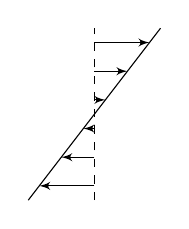
\begin{tikzpicture}[scale=0.7, yscale=1.3]
    \draw (-1.2, -1.2) -- (1.2, 1.2);

    \draw [dashed] (0, -1.2) -- (0, 1.2);

    \foreach \x in {1, 0.6, 0.2, -0.2, -0.6, -1}{
      \draw [-latex'] (0, \x) -- (\x, \x);
    }
  \end{tikzpicture}
\end{center}
Recall that the $z$-direction vorticity is given by
\[
  \omega_3 = \frac{\partial v}{\partial x} - \frac{\partial u}{\partial y},
\]
and evolves as
\[
  \frac{\partial \omega_3}{\partial t} + U \frac{\partial \omega_3}{\partial x} = U' \left(\frac{\partial u}{\partial x} + \frac{\partial v}{\partial y}\right) + v U'' + \frac{1}{Re} \nabla^2 \omega_3.
\]
Assuming constant shear and $\beta = 0$ at high Reynolds number, we have $\frac{\D \omega_3}{\D t} \simeq 0$.

Suppose we have some striped patch of vorticity:
\begin{center}
  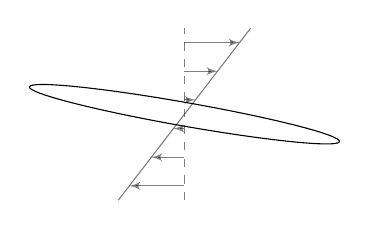
\begin{tikzpicture}
    \draw[rotate=-10] ellipse (2 and 0.15);
    \begin{scope}[scale=0.7, yscale=1.3, opacity=0.5]
      \draw (-1.2, -1.2) -- (1.2, 1.2);
    \draw [dashed] (0, -1.2) -- (0, 1.2);
      \foreach \x in {1, 0.6, 0.2, -0.2, -0.6, -1}{
        \draw [-latex'] (0, \x) -- (\x, \x);
      }
    \end{scope}
  \end{tikzpicture}
\end{center}
In this stripe, we always have $\omega_3 > 0$. Now over time, due to the shear flow, this evolves to become something that looks like
\begin{center}
  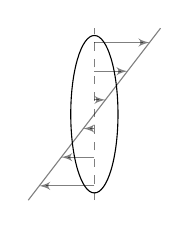
\begin{tikzpicture}
    \draw[rotate=90] ellipse (1 and 0.3);
    \begin{scope}[scale=0.7, yscale=1.3, opacity=0.5]
      \draw (-1.2, -1.2) -- (1.2, 1.2);
    \draw [dashed] (0, -1.2) -- (0, 1.2);
      \foreach \x in {1, 0.6, 0.2, -0.2, -0.6, -1}{
        \draw [-latex'] (0, \x) -- (\x, \x);
      }
    \end{scope}
  \end{tikzpicture}
\end{center}
Now by incompressibility, the area of this new region is the same as the area of the old. We also argued that $\omega_3$ does not change. So the total quantity $\int_\mathcal{D} \omega_3 \;\d A = \int_\mathcal{D} \nabla \times \mathbf{u} \cdot \d A$ does not change. But Stokes' theorem says
\[
  \int_{\mathcal{D}} \nabla \times \mathbf{u} \cdot \d A = \int_{\partial \mathcal{D}} \mathbf{u} \cdot \;\d \ell.
\]
Since the left-hand-side didn't change, the same must be true for the right hand side. But since the boundary $\partial \mathcal{D}$ decreased in length, this implies $\mathbf{u}$ must have increased in magnitude! This growth is only transient, since after some further time, the vorticity patch gets sheared into
\begin{center}
  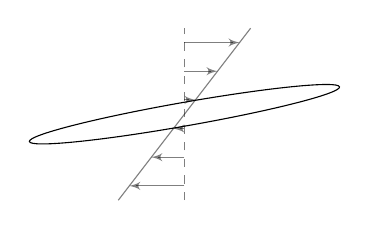
\begin{tikzpicture}
    \draw[rotate=10] ellipse (2 and 0.15);
    \begin{scope}[scale=0.7, yscale=1.3, opacity=0.5]
      \draw (-1.2, -1.2) -- (1.2, 1.2);
    \draw [dashed] (0, -1.2) -- (0, 1.2);
      \foreach \x in {1, 0.6, 0.2, -0.2, -0.6, -1}{
        \draw [-latex'] (0, \x) -- (\x, \x);
      }
    \end{scope}
  \end{tikzpicture}
\end{center}
But remember that Stokes theorem tells us
\[
  \int_\mathcal{D} [\nabla \times \mathbf{u}] \;\d A = \int_{\partial D} \mathbf{u} \cdot \d \ell.
\]
Thus, if we have vortices that are initially tilted into the shear, then this gets advected by the mean shear. In this process, the perimeter of each vortex sheet gets smaller, then grows again. Since $\int_{\partial \mathcal{D}} \mathbf{u} \cdot \d \ell$ is constant, we know $\mathbf{u}$ grows transiently, and then vanishes again.

\subsubsection*{Lift up}
Another mechanism is lift-up. This involves doing some mathematics. Suppose we instead expand our solutions as
\[
  v = \tilde{v}(y, t) e^{i\alpha x + i \beta z},\quad \eta = \tilde{\eta}(y, t) e^{i\alpha x + i \beta z}.
\]
Focusing on the $\alpha = 0$ and $Re = \infty$ case, the Orr-Sommerfeld and Squire equations are
\begin{align*}
  \frac{\partial}{\partial t} \tilde{\eta}(y, t) &= -i\beta U' \tilde{v}\\
  \frac{\partial}{\partial t} (\mathcal{D}^2 - k^2) \tilde{v} &= 0.
\end{align*}
Since we have finite depth, except for a few specific values of $k$, the only solution to the second equation is $\tilde{v}(y, t) = \tilde{v}_0(y)$, and then
\[
  \tilde{\eta} = \tilde{\eta}_0 - i \beta U' \tilde{v}_0 t.
\]
This is an algebraic instability. The constant $\tilde{v}(y, t)$ means fluid is constantly being lifted up, and we can attribute this to the effects of the $\omega_1$ of streamwise rolls.

%Recall the Squire equation in the large Re limit:
%\[
%  \left[\frac{\partial}{\partial t} + i \alpha U \right] \tilde{\eta}(y, t) = -i \beta U' \tilde{v}(y, t),
%\]
%where we set
%\[
%  v = \tilde{v}(y, t) e^{i\alpha x + i \beta z},\quad \eta = \tilde{\eta}(y, t) e^{i\alpha x + i \beta z}.
%\]
%We can formally integrate
%\[
%  \tilde{\eta} = \tilde{\eta}_0 e^{-i\alpha Ut} - i \beta U' e^{-i\alpha Ut} \int_0^t \tilde{v}(y, \tau)e^{i \alpha U\tau} \;\d \tau.
%\]
%Let's suppose that $\alpha = 0$. Then the evolution is completely dominated by wall-normal velocity. We make similar assumptions for the Rayleigh equation, which was
%\[
%  \left[\left(\frac{\partial}{\partial t} + i \alpha U\right) (\mathcal{D}^2 - k^2) - i \alpha U''\right] \tilde{v}(y, t) = 0.
%\]
%If $\alpha = 0$, then $\tilde{v} = \tilde{v}_0$ is a constant, and so $\tilde{\eta} = \tilde{\eta}_0 - i \beta U' \tilde{v}_0 t$. This is an \emph{algebraic} instability. Such dynamics can be associated with streamwise rolls with purely $\omega_1$ \emph{lifting up} fluid.

We should be a bit careful when we consider the case where the disturbance is localized. In this case, we should consider quantities integrated over all $x$. We use a bar to denote this integral, so that, for example, $\bar{v} = \int_{-\infty}^\infty v\;\d x$. Of course, this makes sense only if the disturbance is local, so that the integral converges. Ultimately, we want to understand the growth in the energy, but it is convenient to first understand $\bar{v}, \bar{u}$, and the long-forgotten $\bar{p}$. We have three equations
\begin{align*}
  \nabla^2 p &= - 2U' \frac{\partial v}{\partial x}\\
  \frac{\partial v}{\partial t} + U \frac{\partial v}{\partial x} &= - \frac{\partial p}{\partial y}\\
  \frac{\partial u}{\partial t} + U \frac{\partial u}{\partial x} + v U' &= - \frac{\partial p}{\partial x}.
\end{align*}
Note that $U$ does not depend on $x$, and all our (small lettered) variables vanish at infinity since the disturbance is local. Thus, integrating the first equation over all $x$, we get $\nabla^2 \bar{p} = 0$. So $\bar{p} = 0$. Integrating the second equation then tells us $\frac{\partial \bar{v}}{\partial t} = 0$. Finally, plugging this into the integral of the last equation tells us
\[
  \bar{u} = \bar{u}_0 - \bar{v}_0 U' t.
\]
Thus, $\bar{u}$ grows linearly with time. However, this does not immediately imply that the energy is growing, since the domain is growing as well, and the velocity may be spread over a larger region of space.

Let's suppose $u(x, 0) = 0$ for $|x| > \delta$. Then at time $t$, we would expect $u$ to be non-zero only at $U_{min} t - \delta < x < U_{max} t + \delta$. Recall that Cauchy--Schwarz says
\[
  \left|\int_{-\infty}^\infty f(x) g(x)\;\d x \right|^2 \leq \left(\int_{-\infty}^\infty |f(x)|^2\;\d x\right)\left(\int_{-\infty}^\infty |g(x)|^2 \;\d x\right).
\]
Here we can take $f = u$, and
\[
  g(x) =
  \begin{cases}
    1 & U_{min} t - \delta < x < U_{max} t + \delta\\
    0 & \text{otherwise}
  \end{cases}.
\]
Then applying Cauchy--Schwarz gives us
\[
  \bar{u}^2 \leq [\Delta U + t + 2\delta] \int_{-\infty}^\infty u^2 \;\d x.
\]
So we can bound
\[
  E \geq \frac{[\bar{u}]^2}{2 \Delta U}t = \frac{[\bar{v}_0 U']^2 t}{2 \Delta U}
\]
provided $t \gg \frac{2\delta}{\Delta U}$. Therefore energy grows at least as fast as $t$, but not necessarily as fast as $t^2$.


%Let's try to recall some linear algebra. We shall consider bounded domains, so that we don't have to worry about continuous spectra. Let us also assume that finite Fourier representations of a perturbation are adequate. Further, let us assume that the base state is independent of time, to make life easier.
%
%For a weight matrix $W$, we can define a weighted inner product by
%\[
%  (\mathbf{a}, \mathbf{b}) = \mathbf{a}^\dagger W\mathbf{b},
%\]
%where $\mathbf{a}, \mathbf{b} \in \C^n$. Since the weight matrix is positive definite, we have a \term{Cholesky factorization} $W = FF^\dagger$, where $F$ is lower triangular. We now have a natural definition of an (energy) norm:
%\[
%  \|\mathbf{q}(t)\|^2 = (\mathbf{q}, \mathbf{q}) = \mathbf{q}^\dagger W\mathbf{q} = \|F^\dagger \mathbf{q}(t)\|_2^2.
%\]
%Of course, if $W$ is just the identity matrix, then we are doing nothing. What this tells us is that we can always change our coordinate system so that we get the Euclidean norm, so let us assume that is the case. In particular, this removes problems to do with $\mathcal{D} = \frac{\partial}{\partial y}$.
%
%In this case, we can reduce the stability problem to solving a system of coupled linear ODEs. But unlike classic undergraduate problems, our operators are not normal.
%
%We are interested in a system
%\[
%  \frac{\d \mathbf{q}}{\d t} = L \mathbf{q}
%\]
%for $\mathbf{q} \in \C^n$ and $\mathbf{q}(0) = \mathbf{q}_0$. We can solve this in terms of matrix exponentials:
%\[
%  \mathbf{q}(t) = e^{Lt} \mathbf{q}_0,
%\]
%where the matrix exponential is defined by
%\[
%  e^{Lt} = 1 + Lt + \frac{t^2}{2} L^2 + \cdots.
%\]
%The key question is what is the maximum gain
%\[
%  G(t) = \max_{\mathbf{q}(0) \not= 0}\frac{\|\mathbf{q}(t)\|^2}{ \|\mathbf{q}(0)\|^2} = \max_{\mathbf{q}(0) \not= 0} \frac{\|e^{Lt} \mathbf{q}(0)\|^2}{\|\mathbf{q}(0)\|^2}.
%\]
%By definition, this is the natrix norm:
%\begin{defi}[Matrix norm]\index{matrix norm}
%  Let $B$ be an $n \times n$ matrix. Then the \emph{matrix norm} is
%  \[
%    \|B\| = \max_{\mathbf{v} \not= 0} \frac{\|B\mathbf{v}\|}{\|\mathbf{v}\|}.
%  \]
%\end{defi}
%The fundamental issue is then to describe $q$ in terms of normalized eigenvectors of $L$. We order the associated eigenvalues by their real partrs, so that $\Re(\lambda_1) \geq \cdots \geq \Re(\lambda_n)$. Then the gain is clearly bounded below by
%\[
%  G(t) \geq e^{2 \Re(\lambda_1)t}.
%\]
%If $L$ is normal, then the eigenvectors form an orthonormal basis. So we can write $L = V \Lambda V^{-1}$ for $\Lambda = \diag(\lambda_1,\ldots, \lambda_n)$ and $V$ is unitary. Then % condition number \kappa(V) = 1, but in general \kappa(V) = |V| |V^{-1}|
%\[
%  G(t) = \|e^{Lt}\|^2 = \|V e^{\Lambda t} V^{-1}\|^2 = \|e^{\Lambda t}\|^2 = e^{2 \Re (\lambda_1) t}.
%\]
%By life gets enormously more complicated when matrices are non-normal. Recall the \term{condition number}
%\[
%  \kappa(A) = \|A\| \|A^{-1}\|.
%\]
%Singluar values and singular vectors air pairs of vectors $(\mathbf{v}, \mathbf{u})$ such that
%\[
%  A\mathbf{v} = \sigma \mathbf{u},\quad A^\dagger \mathbf{u} = \sigma \mathbf{v}.
%\]
%Then we have
%\[
%  A^\dagger A \mathbf{v} = \sigma^2 \mathbf{v},\quad AA^\dagger \mathbf{u} = \sigma^2 \mathbf{u}.
%\]
%Note $AA^\dagger$ and $A^\dagger A$. We may wlog assume singular values are normalized, so that $\|A\|= \sigma_{max}$, but consider the square invertible case:
%\[
%  A^{-1}A \mathbf{v} = \sigma A^{-1} \mathbf{u},\quad (A^{-1})^\dagger A^\dagger \mathbf{u} = \sigma [A^{-1}]^{\dagger} \mathbf{v}.
%\]
%Sio in fact we have
%\[
%  \frac{1}{\sigma} \mathbf{v} = A^{-1} \mathbf{u},\quad \frac{1}{\sigma} \mathbf{u} = [A^\dagger]^{-1} \mathbf{v}.
%\]
%Therefore we know
%\[
%  \|A^{-1}\| = \frac{1}{\sigma_{min}}.
%\]
%So we have
%\[
%  \kappa(A) = \frac{\sigma_{max}}{\sigma_{min}}.
%\]
%Therefore, returning to gain, where now eigenvectors do not form orthonormal basis, we have (with $V$ not necessarily unitary)
%\[
%  G(t) = \|e^{Lt}\|^2 = \|V e^{\Lambda t} V^{-1}\|^2 \leq \|V\|^2 \|e^{\Lambda t}\|^2 \|V^{-1}\|^2 = \kappa^2(V) e^{2 \Re(\lambda_1) t},
%\]
%which may be much larger. So we have the possibility for transient growth.
%
%Actually to calculate transient growth, it is very tempting to use the idea of SVD. We can write $e^{Lt} = B$, with
%\[
%  BV = U\Sigma, U^\dagger = U^{-1}, V^\dagger = V^{-1}, \Sigma = \diag(\sigma_1, \ldots, \sigma_n),
%\]
%with $\sigma_i \in \R$ and $\sigma_1 > \cdots > \sigma_n \geq 0$.
%
%Therefore, $B\mathbf{v}_1 = \sigma_1 \mathbf{u}_1$, and remembering the definition of matrix norms, we have
%\begin{multline*}
%  G(t) =\|e^{Lt}\|^2 = \max_{\mathbf{x} \not= 0} \frac{(B\mathbf{x}, B\mathbf{x})}{(\mathbf{x}, \mathbf{x}}) = \max_{\mathbf{x} \not= 0} \frac{(U\Sigma V^\dagger \mathbf{x}, U\Sigma V^\dagger \mathbf{x})}{(\mathbf{x}, \mathbf{x})}\\
%  = \max_{\mathbf{x} \not= 0} \frac{(\Sigma V^\dagger \mathbf{x}, \Sigma V^\dagger \mathbf{x})}{(\mathbf{x}, \mathbf{x})} = \max_{\mathbf{y} \not= 0} \frac{(\Sigma \mathbf{y}, \Sigma \mathbf{y})}{(\mathbf{y}, \mathbf{y})} = \sigma_1^2(t).
%\end{multline*}
%The optimal initial condition is $\mathbf{v}_1$, power and appealing techniques, as SVD can be calculated. This can of course be applied to the Orr-Sommerfeld equation, but there are subtleties arising from discretization.
%
%% say a bit more
%But there are some further problems. Crucially, this assumes the system is linear.

\section{A variational point of view}
In this chapter, we are going to learn about a more robust and powerful way to approach and understand transient growth. Instead of trying to think about $G(t)$ as a function of $t$, let us fix some target time $T$, and just look at $G(T)$.

For any two times $t_i < t_f$, we can define a \term{propagator function} such that
\[
  \mathbf{u}(t_f) = \Phi(t_f, t_i) \mathbf{u}(t_i)
\]
for any solution $\mathbf{u}$ of our equations. In the linear approximation, this propagator is a linear function between appropriate function spaces. Writing $\Phi = \Phi(T, T_0)$, the gain problem is then equivalent to maximizing
\begin{multline*}
  G(T, T_0) = \frac{E(T)}{E(T_0)} = \frac{\bra \mathbf{u}_p(T), \mathbf{u}_p(T)\ket}{ \bra \mathbf{u}_p(T_0), \mathbf{u}_p(T_0)\ket}\\
  = \frac{\bra \Phi \mathbf{u}_p(T_0), \Phi \mathbf{u}_p(T_0)\ket}{\bra \mathbf{u}_p(T_0), \mathbf{u}_p(T_0)\ket} = \frac{\bra \mathbf{u}_p(T_0), \Phi^\dagger \Phi \mathbf{u}_p(T_0)\ket}{\bra \mathbf{u}_p(T_0), \mathbf{u}_p(T_0)\ket}.
\end{multline*}
Here the angled brackets denote natural inner product leading to the energy norm. Note that the operator $\Phi^\dagger \Phi$ is necessarily self-adjoint, and so this $G$ is maximized when $\mathbf{u}_p(T_0)$ is chosen to be the eigenvector of $\Phi$ of maximum eigenvalue.

There is a general method to find the maximum eigenvector of a (self-adjoint) operator $\Phi$. We start with a random vector $\mathbf{x}$. Then we have $\Phi^n \mathbf{x} \sim \lambda_1^n \mathbf{v}_1$ as $n \to \infty$, where $\lambda_1$ is the maximum eigenvalue with associated eigenvector $\mathbf{v}_1$. Indeed, if we write $x$ as the linear combination of eigenvectors, then as we apply $\Phi$ many times, the sum is dominated by the term with largest eigenvalue.

So if we want to find the mode with maximal transient growth, we only need to be able to compute $\Phi^\dagger \Phi$. The forward propagator $\Phi(T, T_0)$ is something we know how to compute (at least numerically). We simply numerically integrate the Navier--Stokes equation. So we need to understand $\Phi(T, T_0)^\dagger$.

Let $\mathbf{u}(t)$ be a solution to the linear equation
\[
  \frac{\d \mathbf{u}}{\d t}(t) = L(t) \mathbf{u}(t).
\]
Here we may allow $L$ to depend on time. Let $L^\dagger$ be the adjoint, and suppose $\mathbf{v}(t)$ satisfies
\[
  \frac{\d \mathbf{v}}{\d t}(t) = - L(t)^\dagger \mathbf{v}(t).
\]
Then the chain rule tells us
\[
  \frac{\d}{\d t} \bra\mathbf{v}(t), \mathbf{u}(t)\ket = \bra -L(t)^\dagger \mathbf{v}(t), \mathbf{u}(t)\ket + \bra \mathbf{v}(t), L(t)^\dagger \mathbf{u}(t)\ket = 0.
\]
So we know that
\[
  \bra \mathbf{v}(T_0), \mathbf{u}(T_0)\ket = \bra \mathbf{v}(T), \mathbf{u}(T)\ket = \bra \mathbf{v}(T), \Phi(T, T_0) \mathbf{u}(T_0)\ket.
\]
Thus, given a $\mathbf{v}_0$, to compute $\Phi(T, T_0)^\dagger \mathbf{v}_0$, we have to integrate the adjoint $\frac{\d \mathbf{v}}{\d t} = - L(t)^\dagger v$ \emph{backwards in time}, using the ``initial'' condition $\mathbf{v}(T) = \mathbf{v}_0$, and then we have
\[
  \Phi(T, T_0)^\dagger \mathbf{v}_0 = \mathbf{v}(T_0).
\]
What does the adjoint equation look like? For a time-dependent background shear flow, the linearized forward/direct equation for a perturbation $\mathbf{u}_p$ is given by
\[
  \frac{\partial \mathbf{u}_p}{\partial t} + (\mathbf{U}(t) \cdot \nabla) \mathbf{u}_p = -\nabla p_p - (\mathbf{u}_p \cdot \nabla) \mathbf{u}(t) + Re^{-1} \nabla^2 \mathbf{u}_p.
\]
The adjoint (linearized) Navier--Stokes equation is then
\[
  -\frac{\partial \mathbf{u}_a}{\partial t} = \boldsymbol\Omega \times \mathbf{u}_a - \nabla \times (\mathbf{U} \times \mathbf{u}_\sigma) - \nabla p_a + Re^{-1} \nabla^2 \mathbf{u}_a,
\]
where we again have
\[
  \nabla \cdot \mathbf{u}_a = 0,\quad \boldsymbol\Omega = \nabla \times \mathbf{U}.
\]
This PDE is ill-posed if we wanted to integrate it forwards in time, but that does not concern us, because to compute $\Phi^\dagger$, we have to integrate it \emph{backwards} in time.

Thus, to find the maximal transient mode, we have to run the \term{direct-adjoint loop}.
\[
  \begin{tikzcd}
    \mathbf{u}_p(T_0) \ar[r, "\Phi"] & \mathbf{u}_p(T) \ar[d]\\
    \Phi^\dagger \Phi (\mathbf{u}_p(T_0)) \ar[u, dashed] & \mathbf{u}_p(T) \ar[l, "\Phi^\dagger"]
  \end{tikzcd},
\]
and keep running this until it converges.

Using these analysis, we can find some interesting results. For example, in a shear layer flow, 3-dimensional modes with both streamwise and spanwise perturbations are the most unstable. However, in the long run, the Kelvin-Helmholtz modes dominate.

%Why does this work? And how does this relate to the toy problems we were looking at before? Let's think about a simple linear version first with energy norms:
%\[
%  \frac{\partial \mathbf{q}}{\partial t} = \mathcal{L} \mathbf{q}.
%\]
%Then it is again straightforward to define the adjoint operator $\mathcal{L}^\dagger$, and the eigenvalues of $\mathcal{L}^\dagger$ are thus complex conjugates of the eigenvalues of $\mathcal{L}$. We denoted the associated eigenvectors of $\mathcal{L}$ as $\mathbf{v}_k^{(d)}$ and of $\mathcal{L}^\dagger$ as $\mathbf{v}_k^{(a)}$. We have biorthogonality property
%\[
%  (\mathbf{v}_i^{(a)}, \mathbf{v}_j^{(d)} = 0 \text{ if }i \not= j.
%\]
%The normalized initial condition approximation is then
%\[
%  \mathbf{q}(0) = \sum_{k = 1}^n \alpha_k \mathbf{v}_k^{(d)},\quad \alpha_k = \frac{(\mathbf{v}_k^{(a)}, \mathbf{q})}{(\mathbf{v}_k^{(a)}, \mathbf{v}_k^{(d)}}.
%\]
%If there is a dominant mode within the system $\mathbf{v}_1^{(d)}$, and the system is strongly non-normal so that $(\mathbf{v}_1^{(a)}, \mathbf{v}_1^{(d)}) \ll 1$ (as in the toy problem), then $\alpha_k$ would be very large, and so there can be very strong amplification. In fact, the optimal initial condition should be the equivalent eigenvector of the adjoint, $\mathbf{v}_k^{(a)}$.
%
%But the adjoint is even more attractive if we pose it a variational way\ldots

\subsubsection*{Variational formulation}
We can also use variational calculus to find the maximally unstable mode. We think of the calculation as a \emph{constrained optimization} problem with the following requirements:
\begin{enumerate}
  \item For all $T_0 \leq t \leq T$, we have $\frac{\partial \mathbf{q}}{\partial t} = \mathcal{D}_t \mathbf{q} = \mathcal{L} \mathbf{q}$.
  \item The initial state is given by $\mathbf{q}(0) = \mathbf{q}_0$.
\end{enumerate}
We will need Lagrangian multipliers to impose these constraints, and so the augmented Lagrangian is
\[
  \mathcal{G} = \frac{\bra \mathbf{q}_T, \mathbf{q}_T\ket}{\bra \mathbf{q}_0, \mathbf{q}_0\ket} - \int_0^T \bra \tilde{\mathbf{q}},  (\mathcal{D}_t - \mathcal{L}) \mathbf{q}\ket \;\d t + \bra \tilde{\mathbf{q}}_0, \mathbf{q}(0) - \mathbf{q}_0\ket.
\]
Taking variations with respect to $\tilde{\mathbf{q}}$ and $\tilde{\mathbf{q}}_0$ recover the evolution equation and the initial condition. The integral can then be written as
\[
  \int_0^T \bra \tilde{\mathbf{q}}, (\mathcal{D}_t - \mathcal{L})\mathbf{q}\ket \;\d t = \int_0^T \bra \mathbf{q}, (\mathcal{D}_t + \mathcal{L}^\dagger) \tilde{\mathbf{q}}\ket \;\d t + \bra \tilde{\mathbf{q}}_0, \mathbf{q}_0\ket - \bra \tilde{\mathbf{q}}_T, \mathbf{q}_T\ket.
\]
Now if we take a variation with respect to $\mathbf{q}$, we see that $\tilde{\mathbf{q}}$ has to satisfy
\[
  (\mathcal{D}_t + \mathcal{L}^\dagger) \tilde{\mathbf{q}} = 0.
\]
So the Lagrange multiplier within such a variational problem evolves according to the adjoint equation!

Taking appropriate adjoints, we can write
\[
  \mathcal{G} = \frac{\bra \mathbf{q}_T, \mathbf{q}_T\ket}{\bra \mathbf{q}_0, \mathbf{q}_0\ket} + \int_0^T \bra \mathbf{q}, (\mathcal{D}_t + \mathcal{L}^\dagger) \tilde{\mathbf{q}}\ket \;\d t + \bra \tilde{\mathbf{q}}_0, \mathbf{q}_0\ket - \bra \tilde{\mathbf{q}}_T, \mathbf{q}_T\ket + \text{boundary terms}.
\]
But if we take variations with respect to our initial conditions, then $\frac{\delta \mathcal{G}}{\delta \mathbf{q}_0} = 0$ gives
\[
  \tilde{\mathbf{q}}_0 = \frac{2 \bra \mathbf{q}_T, \mathbf{q}_T\ket}{\bra \mathbf{q}_0, \mathbf{q}_0\ket^2} \mathbf{q}_0.
\]
Similarly, setting $\frac{\delta \mathcal{G}}{\delta \mathbf{q}_T} = 0$, we get
\[
  \tilde{\mathbf{q}}_T = \frac{2}{\bra \mathbf{q}_0, \mathbf{q}_0\ket }\mathbf{q}_T.
\]
Applying $\bra \ph, \mathbf{q}_0\ket$ to the first equation and $\bra \ph, \mathbf{q}_T\ket$ to the second, we find that
\[
  \bra \tilde{\mathbf{q}}_0, \mathbf{q}_0\ket = \bra \tilde{\mathbf{q}}_T, \mathbf{q}_T\ket.
\]
This is the equation we previously saw for the adjoint equation, and this provides a consistency condition to see if we have found the optimal solution.

Previously our algorithm used power iteration, which requires us to integrate forwards and backwards many times. However, we now have \emph{gradient information} for gain:
\[
  \frac{\delta \mathcal{G}}{\partial \mathbf{q}_0} = \tilde{\mathbf{q}}_0 - \frac{2 \bra \mathbf{q}_T, \mathbf{q}_T\ket}{\bra \mathbf{q}_0, \mathbf{q}_0\ket^2}\mathbf{q}_0.
\]
This allows us to exploit optimization algorithms (steepest descent, conjugate gradient etc.). This has an opportunity for faster convergence.

There are many ways we can modify this. One way is to modify the inner product. Note that we actually had to use the inner product in three occasions:
\begin{enumerate}
  \item Inner product in the objective functional $\mathcal{J}$
  \item Inner product in initial normalization/constraint of the state vector.
  \item Inner product in the definition of adjoint operator.
\end{enumerate}
We used the same energy norm for all of these, but there is no reason we have to use the same norm for all of these. However, there are strong arguments that an energy norm is natural for norm 2. It is a wide open research question as to whether there is an appropriate choice for inner product 3. On the other hand, investigation of variation of inner product 1 has been widely explored.

As an example, consider $p$-norms
\[
  \mathcal{J} = \left( \frac{1}{V_\Omega} \int_\Omega e(x, T)^p \;\d \Omega\right)^{1/p},\quad e(x, T) = \frac{1}{2} |u(x, T)|^2. % tilde is dagger everywhere
\]
This has the attraction that for large values of $p$, this would be dominated by peak values of $e$, not average.

When we set $p = 1$, i.e.\ we use the usual energy norm, then we get a beautiful example of the Orr mechanism, in perfect agreement with what SVD tells us. For, say, $p = 50$, we get more exotic center/wall modes. % insert pictures ?

%Replacing the energy term in $\mathcal{G}$ with $\mathcal{J}$, we obtain 
%Then we have
%\[
%  \mathcal{M} = \mathcal{J} - \int_0^T \left\bra \mathbf{u}^\dagger, \left(\frac{\partial \mathbf{u}}{\partial t} + \mathbf{u} \cdot \nabla \mathbf{u} + \mathbf{u} \cdot \nabla \mathbf{U} + \nabla p - \frac{1}{Re} \nabla^2 \mathbf{u}\right)\right\ket - \bra \mathbf{p}^\dagger, \nabla \cdot \mathbf{u}\ket \;\d t - \bra \mathbf{u}^\dagger_0, \mathbf{u}_0 - \mathbf{u}(0)\ket.
%\]
%Note that the pressure is a Lagrange multiplier.
%
%Here integration by parts with respect to time will lead to a term $\bra \tilde{\mathbf{u}} (0), \mathbf{u}(0)\ket - \bra \tilde{\mathbf{u}} (T), \mathbf{u}(T)\ket$. Variations with respect to $\mathbf{u}(0)$ , $\mathbf{u}(T)$ lead to interesting alternate conditions. We have
%\[
%  \frac{\delta \mathcal{M}}{\delta \mathbf{u}_0} = \tilde{\mathbf{u}}_0.
%\]
%If we fix the norm of $\mathbf{u}_0$, then given $\frac{\delta \mathcal{M}}{\delta \mathbf{u}_0}$, we should ``improve'' our solution by letting $\mathbf{u}_0$ move in the direction of the projection of $\frac{\delta \mathcal{M}}{\delta \mathbf{u}_0}$ to the sphere of fixed norm. So the optimal solution occurs when $\tilde{\mathbf{u}}_0, \mathbf{u}_0$ are perfectly parallel.
%
%If we set $\frac{\delta \mathcal{M}}{\delta \mathbf{u}_T} = 0$, then we have
%\[
%  \tilde{\mathbf{u}} (x, T) = \left(\frac{1}{V_\Omega} \int_\Omega e(x, T)^p \;\d \Omega\right)^{1/p - 1} e(x, T)^{p - 1} \mathbf{u}(x, T).
%\]
%So although there is a term $\bra \mathbf{u}^\dagger(0), \mathbf{u}(0)\ket - \bra \tilde{\mathbf{u}}(T), \mathbf{u}(T)\ket$, it doesn't affect the value of $\mathcal{M}$. Iterative process leads to optimal solutions for different objective functional.
%
%Therefore convergence occurs when $\tilde{\mathbf{u}}_0$, $\mathbf{u}_0$ are perfectly parallel if $\mathbf{u}_0$ is normalized.

\subsubsection*{Non-linear adjoints}
In the variational formulation, there is nothing in the world that stops us from using a non-linear evolution equation! We shall see that this results in slightly less pleasant formulas, but it can still be done.

Consider plane Couette flow with $Re = 1000$, and allow arbitrary amplitude in perturbation
\[
  \mathbf{u}_{tot} = \mathbf{U} + \mathbf{u},\quad \partial_t \mathbf{u} + (\mathbf{u} + \mathbf{U}) \cdot \nabla (\mathbf{u} + \mathbf{U}) = - \nabla p + Re^{-1} \nabla^2 \mathbf{u},
\]
where $\mathbf{U} = y\hat{x}$. We can define a variational problem with Lagrangian
\[
  \mathcal{L} = \frac{E(T)}{E_0} - [\partial_t \mathbf{u} + \mathcal{N}(u) + \nabla p, v] - [\nabla \cdot \mathbf{u}, q] - \left(\frac{1}{2} \bra \mathbf{u}_0, \mathbf{u}_0\ket - E_0\right) c - \bra \mathbf{u}(0) - \mathbf{u}_0, \mathbf{v}_0\ket,
\]
where
\[
  N(u_i) = U_j \partial_j u_i + u_i \partial_i U_j + u_j \partial_j u_i - \frac{1}{Re} \partial_j \partial_j \mathbf{u}_i,\quad [\mathbf{v}, \mathbf{u}] = \frac{1}{T} \int_0^T \bra \mathbf{v}, \mathbf{u}\ket\;\d t.
\]
Variations with respect to the direct variable $u$ can once again define a non-linear adjoint equation
\[
  \frac{\delta \mathcal{L}}{\delta \mathbf{u}} = \partial_t \mathbf{v} + N^\dagger (\mathbf{v}, \mathbf{u}) + \nabla q + \left.\left(\frac{\mathbf{u}}{E_0} - \mathbf{v}\right)\right|_{t = T} + (v - \mathbf{v}_0)|_{t = 0} = 0,
\]
where
\[
  N^\dagger (v_i, \mathbf{u}) = \partial_j (u_j, v_i) - v_j \partial_i u_j + \partial_j (U_j v_i) - v_j \partial_i U_j - v_j \partial_i U_j + \frac{1}{Re} \partial_j \partial_j v_i.
\]
We also have
\[
  \frac{\delta \mathcal{L}}{\delta p} = \nabla \cdot \mathbf{v} = 0,\quad \frac{\delta \mathcal{L}}{\delta \mathbf{u}_0} = \mathbf{v}_0 - c \mathbf{u}_0 = 0.
\]
Note that the equation for the adjoint variable $v$ depends on the direct variable $u$, but is linear in $v$. Computationally, this means that we need to remember our solution to $\mathbf{u}$ when we do our adjoint loop. If $T$ is large, then it may not be feasible to store all information about $\mathbf{u}$ across the whole period, as that is too much data. Instead, the method of \term{checkpointing} is used:
\begin{enumerate}
  \item Pick ``checkpoints'' $0 = T_0 < \cdots < T_K = T$.
  \item When integrating $\mathbf{u}$, we remember high resolution data for $u(x, T_K)$.
  \item When integrating $v$ backwards in the interval $(T_{K - 1}, T_K)$, we use the data remembered at $T_{K - 1}$ to re-integrate to obtain detailed information about $\mathbf{u}$ in the interval $(T_{k - 1}, T_K)$.
\end{enumerate}
This powerful algorithmic approach allows us to identify \emph{minimal} seed of turbulence, i.e.\ the minimal, finite perturbation required to enter a turbulence mode. Note that this is something that cannot be understood by linear approximations! This is rather useful, because in real life, it allows us to figure out how to modify our system to reduce the chance of turbulence arising.

\printindex
\end{document}
